\cotefile{106}
\scanpage{2}
\margin{$\mathrm{Ho}\,C$\quad \unsure{Cat. d'obj. cofibrants}\quad ?}
Soit $(C,W_e,\mathrm{cof})$ une catégorie satisfaisant \unsure{C1 . C3|C1 : C3} de \uline{Brown}, (\unsure{pour mé. C0}).
\inserted{On suppose qu'il y a objet initial $\varnothing$}
(P. ex on pourrait avoir $\mathrm{cof}=\unsure{\mathrm{cof}_{W_e}}$). Alors il est connu que
\[
W_{\mathrm{Cof}}^{-1}\mathrm{Cof}\longrightarrow W^{-1}C
\]
est une équivalence de catégories.

Pour le voir, on va définir un foncteur en sens inverse (qui sera quasi-inverse)
\[
\Phi:W^{-1}C\longrightarrow W_{\mathrm{Cof}}^{-1}\mathrm{Cof},\quad\text{i.e.}\quad C\longrightarrow W_{\mathrm{Cof}}^{-1}\mathrm{Cof}
\]
qui rend les $u\in W$ invers.

Pour tt $x\in C$, utilisant C3 pour $\varnothing\longrightarrow x$, on trouve
\[
\tilde x\xrightarrow[\sim]{\alpha_x}x\qquad\text{avec}\quad \tilde x\in\mathrm{Cof},\ \alpha_x\in W.
\]
Soit alors $x\xrightarrow{f}y$ dans $C$,
\diagram{\begin{tikzcd}
\tilde x \arrow[d,"\alpha_x"',"\sim"] \arrow[dr,"f\alpha_x"] & \tilde y \arrow[d,"\alpha_y"]\\
x \arrow[r,"f"'] & y
\end{tikzcd}}
considérons
\diagram{\begin{tikzcd}
\unsure{\varnothing} \arrow[r] \arrow[d] & \tilde y \arrow[d,"\alpha_y","\sim"']\\
\tilde x \arrow[r,"f\alpha_x"'] & y
\end{tikzcd}}
appliquons le ``weak lifting lemma'', on trouve
\diagram{\begin{tikzcd}
& \tilde y \arrow[r,hook,"i","\sim"'] \arrow[d,"\unsure{\alpha_y}"',"\sim"] & \tilde y' \arrow[dl,"\unsure{\alpha'_y}","\sim"']\\
\tilde x \arrow[r,"f\alpha_x","g"'] \arrow[urr,bend left=12,"\tilde f"] & y &
\end{tikzcd}}
un relèvement $\tilde f$ \deleted{\unsure{comme un des}} \inserted{de $f\alpha_x$} \deleted{$f\alpha_x$} pas vers $\tilde y$, mais vers $\tilde y'$.

Considérons \unsure{lors|alors}
\[
[i]^{-1}\tilde f:\tilde x\longrightarrow\tilde y\qquad\text{dans }\mathrm{Hom}_{W_{\mathrm{Cof}}^{-1}}(\tilde x,\tilde y).
\]
Je dis qu'il ne dépend pas du choix de $(i,\alpha'_{\unsure{y}},\varphi)$. Pour deux tels choix, on
\diagram{\begin{tikzcd}
& \tilde y'_1\\
\tilde y \arrow[ur,hook,"i_1"] \arrow[dr,hook,"i_2"'] &\\
&\tilde y'_2
\end{tikzcd}}
\unsure{quitte à introduire} $\tilde y'_3=\tilde y'_1\vee_{\tilde y}\tilde y'_2$,
SPS que $\tilde y'_1=\tilde y'_2$, $i_1=i_2$, $\alpha'_1=\alpha'_2$, d'où \unsure{on a deux relèvements} $\varphi_1,\varphi_2$ de $f\alpha_x$ vers \unsure{$\underset{g=f\alpha_x}{y}=\tilde y'$}, \deleted{SPS $=$ \unsure{que $\tilde y$}} et on est ramené (écrivant $y'$ au lieu de $\tilde y'$, $x'$ au lieu de $\tilde x$, mais $x$ cof)
\diagram{\begin{tikzcd}
x' \arrow[r,shift left=.65ex,"\varphi"] \arrow[r,shift right=.65ex,"\psi"'] & y' \arrow[r,"\alpha","\sim"'] & y
\end{tikzcd}}
\diagram{\deleted{\begin{tikzcd}
& \unsure{y'}\ \mathrm{cof} \arrow[d,"\alpha","\sim"']\\
x'\ \mathrm{cof} \arrow[ur,shift left=.65ex,"\varphi"] \arrow[ur,shift right=.65ex,"\psi"'] \arrow[r,"g"'] & y
\end{tikzcd}}}
prouver que si $x',y'\in\mathrm{Cof}$, et $\alpha\varphi=\alpha\psi\deleted{\unsure{g}}$, alors
\[
[\varphi]=[\psi]\quad\text{dans } W_{\mathrm{Cof}}^{-1}\mathrm{Cof}.
\]
\margin{\diagram{\begin{tikzcd}
x' \arrow[r] & y\\
x'\amalg x' \arrow[u,"\nabla_{x'}"] \arrow[r,"(\varphi,\psi)"'] & y' \arrow[u,"\in W"']
\end{tikzcd}}
\diagram{\begin{tikzcd}
x'\ \mathrm{cof} \arrow[r,shift left=.65ex] \arrow[r,shift right=.65ex] & y'\ \mathrm{cof} \arrow[r,very thick] & y
\end{tikzcd}}}
\margin{\diagram{\begin{tikzcd}
\varnothing \arrow[r] & \unsure{x} \arrow[d]\\
& y
\end{tikzcd}}}
Si ce lemme est valable, on trouve un foncteur
\[
\deleted{\unsure{W}}C\longrightarrow W_{\mathrm{Cof}}^{-1}\mathrm{Cof},
\]
car la compatibilité de $u\mapsto\Phi(u)$ aux identités et aux compositions est immédiate.
\mspage{1}

\scanpage{3}
\texttt{DATA SET UTILITY - GENERATE}\hfill\texttt{PAGE 0001}

\texttt{IEB352I WARNING : OUTPUT RECFM/LRECL/BLKSIZE COPIED FROM INPUT}

\texttt{PROCESSING ENDED AT EOD}

\diagram{\begin{tikzcd}
x \arrow[r,hook,"\sim"] \arrow[d,"\sim"'] & x' \arrow[dl,"\sim"]\\
y\deleted{\unsure{y}} \arrow[ur,bend right=18,"\sim"'] &\\
y \arrow[u,"\unsure{w}"'] &
\end{tikzcd}}
\diagram{\begin{tikzcd}
& y \arrow[d,"\sim"'] \arrow[dr,"\sim"] &\\
x \arrow[r] & y' \arrow[dr] & y'' \arrow[d]\\
&&y'''
\end{tikzcd}}
\diagram{\begin{tikzcd}
\unsure{x|a} \arrow[dr] \arrow[dd,bend right=15] & y \arrow[d,"\sim"]\\
& \bar y \arrow[dl,"\sim"'] \arrow[d,"\sim"]\\
\bar y' \arrow[r,hook] & \bar y''
\end{tikzcd}}
\diagram{\begin{tikzcd}
\unsure{x|a} \arrow[r,hook] \arrow[d,equal] & \bar y \arrow[d] & y \arrow[l] \arrow[d,equal]\\
x \arrow[r,hook] \arrow[d,equal] & \unsure{\bar y''} & y \arrow[l,very thick] \arrow[d,equal]\\
x \arrow[r] & \bar y' \arrow[u,very thick] & y \arrow[l]
\end{tikzcd}}
\diagram{\begin{tikzcd} {} \arrow[r] & {} \end{tikzcd}}
\diagram{\begin{tikzcd}
{} \arrow[r,hook] \arrow[d] & {} \arrow[d,"\sim"'] & {} \arrow[l,"\sim"'] \arrow[d]\\
{} \arrow[r,hook] & {} & {} \arrow[l]\\
{} \arrow[r] \arrow[u] & {} \arrow[u] & {} \arrow[l] \arrow[u]
\end{tikzcd}}
\diagram{\begin{tikzcd}x \arrow[r,hook] & {}\end{tikzcd}}
\deleted{$\unsure{x\amalg x}$}
\diagram{\begin{tikzcd}x \arrow[r,very thick] & y\end{tikzcd}}
\diagram{\begin{tikzcd}
x \arrow[r,"\deleted{u}"] \arrow[dr,"u"] \arrow[ddr,"u'"'] & y \arrow[d,equal]\\
& y \arrow[d,equal]\\
& {}
\end{tikzcd}}
\diagram{\begin{tikzcd}x \arrow[r,shift left=.8ex,"u"] \arrow[r,shift right=.8ex,very thick] & y\end{tikzcd}}
\diagram{\begin{tikzcd}
&& y \arrow[dl,"\sim"'] \arrow[dr,"\sim"] \arrow[dd,"\unsure{r}"] &&\\
x \arrow[r,hook,"f"] \arrow[drr,"\unsure{i_1f}"'] & y'_1 && y'_2 & x \arrow[l,"g"'] \arrow[dll,"i_2g"]\\
&& \bar y \arrow[ul,"r_1"] \arrow[ur,"r_2"'] &&
\end{tikzcd}}
\diagram{\begin{tikzcd}
x \arrow[r,"f"] & y &\\
x \arrow[r] & \bar y & y \arrow[l]\\
x \arrow[r,"g"] & y &
\end{tikzcd}}
\diagram{\begin{tikzcd}
x \arrow[r,"f"] \arrow[d,equal] & y \arrow[d,"i","\sim"'] & y \arrow[l,"1"'] \arrow[d,equal]\\
x \arrow[r,"h"] \arrow[d,equal] & \bar y & y \arrow[l,"i"'] \arrow[d,equal]\\
x \arrow[r,"g"] & y \arrow[u,"i"] & y \arrow[l,"1"']
\end{tikzcd}}
\diagram{\begin{tikzcd}
x \arrow[r,shift left=.7ex,"f"] \arrow[r,shift right=.7ex,"g"'] \arrow[dr,"h"'] & y \arrow[d,"i","\sim"']\\
& \bar y
\end{tikzcd}}
\diagram{\begin{tikzcd}{} \arrow[r,leftrightarrow,very thick] & {}\end{tikzcd}}
\diagram{\begin{tikzcd}x \arrow[r,very thick,"\sim"] \arrow[d] & y\\ {} \arrow[ur] &\end{tikzcd}}
\diagram{\begin{tikzcd}
y\vee y \arrow[r] & y &\\
x\vee x \arrow[u,"f\vee g"] \arrow[r,very thick] & C \arrow[u,"h"'] & \deleted{\unsure{x}} \arrow[l,shift left=.7ex,"\deleted{\unsure{g}}"] \arrow[l,shift right=.7ex]
\end{tikzcd}}
\diagram{\begin{tikzcd}x \arrow[r,shift left=.7ex,"\unsure{j_1}"] \arrow[r,shift right=.7ex,"\unsure{j'_2|j_2}"'] & C \arrow[r,"\deleted{g}\ h"] & y\end{tikzcd}}
\diagram{\begin{tikzcd}
a \arrow[dr] & y \arrow[d,"\sim"] \arrow[dr] & {} \arrow[d]\\
& \deleted{\unsure{\bar y}} \arrow[dr,shift left=.4ex] \arrow[dr,shift right=.4ex] & {} \arrow[d,"\sim"]\\
&& {}
\end{tikzcd}}
\diagram{\begin{tikzcd}x. & x\end{tikzcd}}
\diagram{\begin{tikzcd}
a \arrow[r] \arrow[d] & \unsure{a} \arrow[r,shift left=.8ex,"\sim"] \arrow[r,shift right=.8ex] \arrow[d,"\unsure{w}","\sim"'] & \bar x \arrow[dl,very thick,"\sim"]\\
b \arrow[r] \arrow[urr,no head,shorten >=15pt] & y \arrow[ur,"\sim"'] &
\end{tikzcd}}
\diagram{\begin{tikzcd}y & {} \arrow[l]\end{tikzcd}}
\diagram{\begin{tikzcd}y \arrow[r,hook] & {}\end{tikzcd}}
$x$

\deleted{$\unsure{x}$}
\diagram{\begin{tikzcd} & {} \arrow[d]\\ {} \arrow[r,bend right=8] & {}\end{tikzcd}}
\deleted{$\unsure{x}$}
\diagram{\begin{tikzcd}a \arrow[r] & y \arrow[d]\\ & {}\end{tikzcd}}
\diagram{\begin{tikzcd}
x\ \mathrm{cof} \arrow[r,hook] \arrow[dr,hook] & y'\ \mathrm{cof} \arrow[r,"\sim"] \arrow[d,"\sim"'] & y\ \mathrm{cof}\\
& \bar y \arrow[ur,"\sim"] & {} \arrow[l,dashed]
\end{tikzcd}}
\diagram{\begin{tikzcd}
x & {} \arrow[dl,no head] & y &\\
y'\ \mathrm{cof} \arrow[r,very thick,"\sim"] \arrow[dr,"?"'] \arrow[ddd,bend right=10] & \bar y \arrow[ur] \arrow[dr,very thick] &&\\
& \bar y_1 \arrow[r] & y_1 &\\
&&&\\
y_2&&&
\end{tikzcd}}
\diagram{\begin{tikzcd}
x \arrow[dr] && y \arrow[dl,"\sim"'] \arrow[dr,"\sim"] \arrow[dd,"\sim"] &\\
& y' \arrow[dr,bend right=25,"\deleted{\unsure{g}}"'] && y''\\
&& y''' \arrow[ul,bend left=15,"\sim"'] \arrow[ur,"\sim"'] &
\end{tikzcd}}
\diagram{\begin{tikzcd}
\bar y \arrow[r,"\sim"] \arrow[d,"\sim"'] & y' \arrow[dl,bend left=28]\\
y'' \arrow[ur,very thick] &
\end{tikzcd}}
\diagram{\begin{tikzcd}x \arrow[r] & y'\end{tikzcd}}
\diagram{\begin{tikzcd}
& \unsure{\varnothing} \arrow[r,hook] \arrow[d,dashed] & y \arrow[d] \arrow[dl]\\
\unsure{x\amalg x'} \arrow[r,hook] & \tilde y \arrow[r,"\sim"] \arrow[d,very thick] & \bar y \arrow[dl,bend left=12]\\
& \tilde y' \arrow[ur,bend right=10] &
\end{tikzcd}}
\diagram{\begin{tikzcd}
\deleted{\unsure{x}} & y \arrow[d]\\
x \arrow[r,shift left=.7ex] \arrow[r,shift right=.7ex] & \bar y
\end{tikzcd}}
\diagram{\begin{tikzcd}&&y \arrow[d]\\ x \arrow[r,hook] & \bar y' \arrow[r,"\sim"'] & \bar y\end{tikzcd}}
\diagram{\begin{tikzcd}&&& y \arrow[d,very thick,"\sim"]\\ x\amalg x \arrow[r,hook] & \deleted{\unsure{x\amalg x}} \arrow[r,hook] & \bar y' \arrow[r,very thick,"\sim"'] & \bar y\end{tikzcd}}
\figure{\begin{tikzpicture}[x=.25cm,y=.25cm]
\draw (0,9) .. controls (5,10.6) and (12.8,15.8) .. (17,18);
\draw (2.6,0) .. controls (10.3,4.3) and (19.8,13.3) .. (27,16.8);
\end{tikzpicture}}
\mspage{2}

\scanpage{4}
\mspage{2}
\diagram{\begin{tikzcd}
\tilde x \arrow[r,"\deleted{\unsure{\varphi}}"] \arrow[d,"\sim"'] \arrow[rr,bend left=22,"\varphi"] & \tilde y \arrow[r,hook,"i","\sim"'] \arrow[d,"\sim"'] \arrow[rrr,bend left=22,"\psi"] & \tilde y' \arrow[dl] & \tilde z \arrow[r,hook,"j","\sim"'] \arrow[d,"\sim"'] & \tilde z' \arrow[dl]\\
x \arrow[r,"f"'] & y \arrow[rr,"g"'] && z &
\end{tikzcd}}
\diagram{\begin{tikzcd}
\unsure{\tilde x} \arrow[dr,bend left=30] & \tilde y \arrow[d,"i"] \arrow[dr,"\psi"] & \tilde z \arrow[d,"j"]\\
&\tilde y'&\tilde z'
\end{tikzcd}}
\diagram{\begin{tikzcd}
\tilde x \arrow[r,"\deleted{\unsure{\tilde f}}"] \arrow[dr,"\tilde f"'] \arrow[ddd,dashed,"\sim"'] & \tilde y \arrow[d,"i_f"] \arrow[dr,"\tilde g"] & \tilde z \arrow[d,"i_g"]\\
& \tilde y' \arrow[dr,no head,"\deleted{\unsure{u}}\ \tilde g'"] \arrow[dd,dashed,"\sim"'] & \tilde z' \arrow[d]\\
&&\tilde z'' \arrow[d,dashed]\\
x \arrow[r,"f"'] & y \arrow[r,"g"'] & z
\end{tikzcd}}

\figure{
\begin{tikzpicture}[x=.35cm,y=.35cm]
\draw (0,0) .. controls (1,-1) and (3,3.6) .. (4,3) .. controls (5,2.4) and (2,-.8) .. (2.1,-.1);
\draw (5,1.1) .. controls (6,2.3) and (7,2.9) .. (8,3.2) .. controls (9,3.5) and (6,0) .. (5.8,-.5);
\end{tikzpicture}}

\deleted{\unsure{En}} Montrons que ce foncteur transforme $f\in W$ en iso.
En effet, si $f\in W$, donc $f\alpha_x\in W$, on voit aussitôt qu'on aura $\tilde f\in W$, donc $[\tilde f]$ est un iso.

Considérons les deux composés
\diagram{\begin{tikzcd}
W_{\mathrm{Cof}}^{-1}\mathrm{Cof} \arrow[r,shift left=1ex,"\Psi"] & W^{-1}C \arrow[l,shift left=1ex,"\Phi"]
\end{tikzcd}}
\deleted{\unsure{faire voir}} \inserted{prouvons} qu'ils \deleted{\unsure{donnent}} sont \deleted{\unsure{égaux}} iso aux foncteurs identiques.

Pour $\Phi\Psi$, cela $=$ l'identité, si on a pris soin de choisir $\tilde x\xrightarrow{\alpha_x}x$ l'identité, quand $x\in\mathrm{Cof}$.
Pour $\Psi\Phi$, il \deleted{suffit de} \inserted{\unsure{va|on va}} voir que le foncteur
\[
\deleted{\unsure{\Psi\Phi\overset{\mathrm{def}}{=}}}\ R\overset{\mathrm{def}}{=}\Psi\Phi\mid C
\]
\[
x\longmapsto\tilde x\qquad C\longrightarrow W^{-1}C
\]
est iso \deleted{à l'identité} \inserted{au foncteur can.}, on a
\[
\underset{\parallel\ \tilde x}{R(x)}\xrightarrow{\unsure{[\alpha_x]}}x\quad\text{dans }C\ \unsure{\text{donc}}\ \text{dans }W^{-1}C\quad(\text{soit }[\alpha_x])
\]
qui est un iso, il faut vérifier que c'est fonctoriel
\diagram{\begin{tikzcd}
\tilde x \arrow[d,"\alpha_x"'] \arrow[rr,bend left=20,"\tilde f"] & \tilde y \arrow[r,hook,"i_f"'] \arrow[d,"\alpha_y"] & \tilde y' \arrow[dl,"\beta_f"]\\
x \arrow[r,"f"'] & y &
\end{tikzcd}}
i.e. qu'on a
\[
[\alpha_y]\deleted{\unsure{\alpha}}([i_f]^{-1}\deleted{\unsure{x}}[\tilde f])=[f][\alpha_x].
\]
Mais $\alpha_y=\beta_f i_f$, d'où le premier mb est $[\beta_f\tilde f]=[f\alpha_x]=[f][\alpha_x]$ cqfd.
\mspage{3}

\scanpage{5}
\texttt{//*\quad DOCUGRA20005}\qquad\unsure{\texttt{I}|\texttt{1}}

\figure{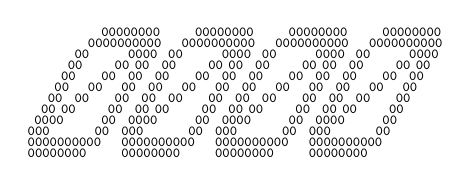
\begin{tikzpicture}[x=.085cm,y=.14cm]
\node[anchor=base west,inner sep=0pt,font=\tiny\ttfamily] at (11,0) {00000000};
\node[anchor=base west,inner sep=0pt,font=\tiny\ttfamily] at (9,-1) {0000000000};
\node[anchor=base west,inner sep=0pt,font=\tiny\ttfamily] at (7,-2) {00};
\node[anchor=base west,inner sep=0pt,font=\tiny\ttfamily] at (15,-2) {0000};
\node[anchor=base west,inner sep=0pt,font=\tiny\ttfamily] at (6,-3) {00};
\node[anchor=base west,inner sep=0pt,font=\tiny\ttfamily] at (13,-3) {00};
\node[anchor=base west,inner sep=0pt,font=\tiny\ttfamily] at (16,-3) {00};
\node[anchor=base west,inner sep=0pt,font=\tiny\ttfamily] at (5,-4) {00};
\node[anchor=base west,inner sep=0pt,font=\tiny\ttfamily] at (11,-4) {00};
\node[anchor=base west,inner sep=0pt,font=\tiny\ttfamily] at (15,-4) {00};
\node[anchor=base west,inner sep=0pt,font=\tiny\ttfamily] at (4,-5) {00};
\node[anchor=base west,inner sep=0pt,font=\tiny\ttfamily] at (9,-5) {00};
\node[anchor=base west,inner sep=0pt,font=\tiny\ttfamily] at (14,-5) {00};
\node[anchor=base west,inner sep=0pt,font=\tiny\ttfamily] at (3,-6) {00};
\node[anchor=base west,inner sep=0pt,font=\tiny\ttfamily] at (7,-6) {00};
\node[anchor=base west,inner sep=0pt,font=\tiny\ttfamily] at (13,-6) {00};
\node[anchor=base west,inner sep=0pt,font=\tiny\ttfamily] at (2,-7) {00};
\node[anchor=base west,inner sep=0pt,font=\tiny\ttfamily] at (5,-7) {00};
\node[anchor=base west,inner sep=0pt,font=\tiny\ttfamily] at (12,-7) {00};
\node[anchor=base west,inner sep=0pt,font=\tiny\ttfamily] at (1,-8) {0000};
\node[anchor=base west,inner sep=0pt,font=\tiny\ttfamily] at (11,-8) {00};
\node[anchor=base west,inner sep=0pt,font=\tiny\ttfamily] at (0,-9) {000};
\node[anchor=base west,inner sep=0pt,font=\tiny\ttfamily] at (10,-9) {00};
\node[anchor=base west,inner sep=0pt,font=\tiny\ttfamily] at (0,-10) {0000000000};
\node[anchor=base west,inner sep=0pt,font=\tiny\ttfamily] at (0,-11) {00000000};
\node[anchor=base west,inner sep=0pt,font=\tiny\ttfamily] at (25,0) {00000000};
\node[anchor=base west,inner sep=0pt,font=\tiny\ttfamily] at (23,-1) {0000000000};
\node[anchor=base west,inner sep=0pt,font=\tiny\ttfamily] at (21,-2) {00};
\node[anchor=base west,inner sep=0pt,font=\tiny\ttfamily] at (29,-2) {0000};
\node[anchor=base west,inner sep=0pt,font=\tiny\ttfamily] at (20,-3) {00};
\node[anchor=base west,inner sep=0pt,font=\tiny\ttfamily] at (27,-3) {00};
\node[anchor=base west,inner sep=0pt,font=\tiny\ttfamily] at (30,-3) {00};
\node[anchor=base west,inner sep=0pt,font=\tiny\ttfamily] at (19,-4) {00};
\node[anchor=base west,inner sep=0pt,font=\tiny\ttfamily] at (25,-4) {00};
\node[anchor=base west,inner sep=0pt,font=\tiny\ttfamily] at (29,-4) {00};
\node[anchor=base west,inner sep=0pt,font=\tiny\ttfamily] at (18,-5) {00};
\node[anchor=base west,inner sep=0pt,font=\tiny\ttfamily] at (23,-5) {00};
\node[anchor=base west,inner sep=0pt,font=\tiny\ttfamily] at (28,-5) {00};
\node[anchor=base west,inner sep=0pt,font=\tiny\ttfamily] at (17,-6) {00};
\node[anchor=base west,inner sep=0pt,font=\tiny\ttfamily] at (21,-6) {00};
\node[anchor=base west,inner sep=0pt,font=\tiny\ttfamily] at (27,-6) {00};
\node[anchor=base west,inner sep=0pt,font=\tiny\ttfamily] at (16,-7) {00};
\node[anchor=base west,inner sep=0pt,font=\tiny\ttfamily] at (19,-7) {00};
\node[anchor=base west,inner sep=0pt,font=\tiny\ttfamily] at (26,-7) {00};
\node[anchor=base west,inner sep=0pt,font=\tiny\ttfamily] at (15,-8) {0000};
\node[anchor=base west,inner sep=0pt,font=\tiny\ttfamily] at (25,-8) {00};
\node[anchor=base west,inner sep=0pt,font=\tiny\ttfamily] at (14,-9) {000};
\node[anchor=base west,inner sep=0pt,font=\tiny\ttfamily] at (24,-9) {00};
\node[anchor=base west,inner sep=0pt,font=\tiny\ttfamily] at (14,-10) {0000000000};
\node[anchor=base west,inner sep=0pt,font=\tiny\ttfamily] at (14,-11) {00000000};
\node[anchor=base west,inner sep=0pt,font=\tiny\ttfamily] at (39,0) {00000000};
\node[anchor=base west,inner sep=0pt,font=\tiny\ttfamily] at (37,-1) {0000000000};
\node[anchor=base west,inner sep=0pt,font=\tiny\ttfamily] at (35,-2) {00};
\node[anchor=base west,inner sep=0pt,font=\tiny\ttfamily] at (43,-2) {0000};
\node[anchor=base west,inner sep=0pt,font=\tiny\ttfamily] at (34,-3) {00};
\node[anchor=base west,inner sep=0pt,font=\tiny\ttfamily] at (41,-3) {00};
\node[anchor=base west,inner sep=0pt,font=\tiny\ttfamily] at (44,-3) {00};
\node[anchor=base west,inner sep=0pt,font=\tiny\ttfamily] at (33,-4) {00};
\node[anchor=base west,inner sep=0pt,font=\tiny\ttfamily] at (39,-4) {00};
\node[anchor=base west,inner sep=0pt,font=\tiny\ttfamily] at (43,-4) {00};
\node[anchor=base west,inner sep=0pt,font=\tiny\ttfamily] at (32,-5) {00};
\node[anchor=base west,inner sep=0pt,font=\tiny\ttfamily] at (37,-5) {00};
\node[anchor=base west,inner sep=0pt,font=\tiny\ttfamily] at (42,-5) {00};
\node[anchor=base west,inner sep=0pt,font=\tiny\ttfamily] at (31,-6) {00};
\node[anchor=base west,inner sep=0pt,font=\tiny\ttfamily] at (35,-6) {00};
\node[anchor=base west,inner sep=0pt,font=\tiny\ttfamily] at (41,-6) {00};
\node[anchor=base west,inner sep=0pt,font=\tiny\ttfamily] at (30,-7) {00};
\node[anchor=base west,inner sep=0pt,font=\tiny\ttfamily] at (33,-7) {00};
\node[anchor=base west,inner sep=0pt,font=\tiny\ttfamily] at (40,-7) {00};
\node[anchor=base west,inner sep=0pt,font=\tiny\ttfamily] at (29,-8) {0000};
\node[anchor=base west,inner sep=0pt,font=\tiny\ttfamily] at (39,-8) {00};
\node[anchor=base west,inner sep=0pt,font=\tiny\ttfamily] at (28,-9) {000};
\node[anchor=base west,inner sep=0pt,font=\tiny\ttfamily] at (38,-9) {00};
\node[anchor=base west,inner sep=0pt,font=\tiny\ttfamily] at (28,-10) {0000000000};
\node[anchor=base west,inner sep=0pt,font=\tiny\ttfamily] at (28,-11) {00000000};
\node[anchor=base west,inner sep=0pt,font=\tiny\ttfamily] at (53,0) {00000000};
\node[anchor=base west,inner sep=0pt,font=\tiny\ttfamily] at (51,-1) {0000000000};
\node[anchor=base west,inner sep=0pt,font=\tiny\ttfamily] at (49,-2) {00};
\node[anchor=base west,inner sep=0pt,font=\tiny\ttfamily] at (57,-2) {0000};
\node[anchor=base west,inner sep=0pt,font=\tiny\ttfamily] at (48,-3) {00};
\node[anchor=base west,inner sep=0pt,font=\tiny\ttfamily] at (55,-3) {00};
\node[anchor=base west,inner sep=0pt,font=\tiny\ttfamily] at (58,-3) {00};
\node[anchor=base west,inner sep=0pt,font=\tiny\ttfamily] at (47,-4) {00};
\node[anchor=base west,inner sep=0pt,font=\tiny\ttfamily] at (53,-4) {00};
\node[anchor=base west,inner sep=0pt,font=\tiny\ttfamily] at (57,-4) {00};
\node[anchor=base west,inner sep=0pt,font=\tiny\ttfamily] at (46,-5) {00};
\node[anchor=base west,inner sep=0pt,font=\tiny\ttfamily] at (51,-5) {00};
\node[anchor=base west,inner sep=0pt,font=\tiny\ttfamily] at (56,-5) {00};
\node[anchor=base west,inner sep=0pt,font=\tiny\ttfamily] at (45,-6) {00};
\node[anchor=base west,inner sep=0pt,font=\tiny\ttfamily] at (49,-6) {00};
\node[anchor=base west,inner sep=0pt,font=\tiny\ttfamily] at (55,-6) {00};
\node[anchor=base west,inner sep=0pt,font=\tiny\ttfamily] at (44,-7) {00};
\node[anchor=base west,inner sep=0pt,font=\tiny\ttfamily] at (47,-7) {00};
\node[anchor=base west,inner sep=0pt,font=\tiny\ttfamily] at (54,-7) {00};
\node[anchor=base west,inner sep=0pt,font=\tiny\ttfamily] at (43,-8) {0000};
\node[anchor=base west,inner sep=0pt,font=\tiny\ttfamily] at (53,-8) {00};
\node[anchor=base west,inner sep=0pt,font=\tiny\ttfamily] at (42,-9) {000};
\node[anchor=base west,inner sep=0pt,font=\tiny\ttfamily] at (52,-9) {00};
\node[anchor=base west,inner sep=0pt,font=\tiny\ttfamily] at (42,-10) {0000000000};
\node[anchor=base west,inner sep=0pt,font=\tiny\ttfamily] at (42,-11) {00000000};
\end{tikzpicture}}

\figure{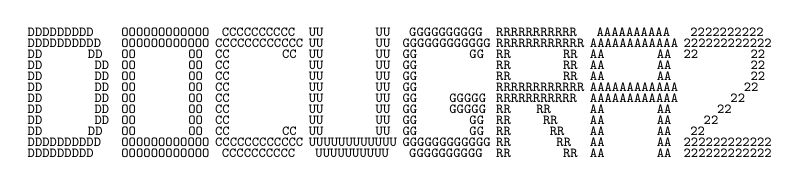
\begin{tikzpicture}[x=.085cm,y=.14cm]
\node[anchor=base west,inner sep=0pt,font=\tiny\ttfamily] at (0,0) {DDDDDDDDD};
\node[anchor=base west,inner sep=0pt,font=\tiny\ttfamily] at (0,-1) {DDDDDDDDDD};
\node[anchor=base west,inner sep=0pt,font=\tiny\ttfamily] at (0,-2) {DD};
\node[anchor=base west,inner sep=0pt,font=\tiny\ttfamily] at (9,-2) {DD};
\node[anchor=base west,inner sep=0pt,font=\tiny\ttfamily] at (0,-3) {DD};
\node[anchor=base west,inner sep=0pt,font=\tiny\ttfamily] at (10,-3) {DD};
\node[anchor=base west,inner sep=0pt,font=\tiny\ttfamily] at (0,-4) {DD};
\node[anchor=base west,inner sep=0pt,font=\tiny\ttfamily] at (10,-4) {DD};
\node[anchor=base west,inner sep=0pt,font=\tiny\ttfamily] at (0,-5) {DD};
\node[anchor=base west,inner sep=0pt,font=\tiny\ttfamily] at (10,-5) {DD};
\node[anchor=base west,inner sep=0pt,font=\tiny\ttfamily] at (0,-6) {DD};
\node[anchor=base west,inner sep=0pt,font=\tiny\ttfamily] at (10,-6) {DD};
\node[anchor=base west,inner sep=0pt,font=\tiny\ttfamily] at (0,-7) {DD};
\node[anchor=base west,inner sep=0pt,font=\tiny\ttfamily] at (10,-7) {DD};
\node[anchor=base west,inner sep=0pt,font=\tiny\ttfamily] at (0,-8) {DD};
\node[anchor=base west,inner sep=0pt,font=\tiny\ttfamily] at (10,-8) {DD};
\node[anchor=base west,inner sep=0pt,font=\tiny\ttfamily] at (0,-9) {DD};
\node[anchor=base west,inner sep=0pt,font=\tiny\ttfamily] at (9,-9) {DD};
\node[anchor=base west,inner sep=0pt,font=\tiny\ttfamily] at (0,-10) {DDDDDDDDDD};
\node[anchor=base west,inner sep=0pt,font=\tiny\ttfamily] at (0,-11) {DDDDDDDDD};
\node[anchor=base west,inner sep=0pt,font=\tiny\ttfamily] at (14,0) {OOOOOOOOOOOO};
\node[anchor=base west,inner sep=0pt,font=\tiny\ttfamily] at (14,-1) {OOOOOOOOOOOO};
\node[anchor=base west,inner sep=0pt,font=\tiny\ttfamily] at (14,-2) {OO};
\node[anchor=base west,inner sep=0pt,font=\tiny\ttfamily] at (24,-2) {OO};
\node[anchor=base west,inner sep=0pt,font=\tiny\ttfamily] at (14,-3) {OO};
\node[anchor=base west,inner sep=0pt,font=\tiny\ttfamily] at (24,-3) {OO};
\node[anchor=base west,inner sep=0pt,font=\tiny\ttfamily] at (14,-4) {OO};
\node[anchor=base west,inner sep=0pt,font=\tiny\ttfamily] at (24,-4) {OO};
\node[anchor=base west,inner sep=0pt,font=\tiny\ttfamily] at (14,-5) {OO};
\node[anchor=base west,inner sep=0pt,font=\tiny\ttfamily] at (24,-5) {OO};
\node[anchor=base west,inner sep=0pt,font=\tiny\ttfamily] at (14,-6) {OO};
\node[anchor=base west,inner sep=0pt,font=\tiny\ttfamily] at (24,-6) {OO};
\node[anchor=base west,inner sep=0pt,font=\tiny\ttfamily] at (14,-7) {OO};
\node[anchor=base west,inner sep=0pt,font=\tiny\ttfamily] at (24,-7) {OO};
\node[anchor=base west,inner sep=0pt,font=\tiny\ttfamily] at (14,-8) {OO};
\node[anchor=base west,inner sep=0pt,font=\tiny\ttfamily] at (24,-8) {OO};
\node[anchor=base west,inner sep=0pt,font=\tiny\ttfamily] at (14,-9) {OO};
\node[anchor=base west,inner sep=0pt,font=\tiny\ttfamily] at (24,-9) {OO};
\node[anchor=base west,inner sep=0pt,font=\tiny\ttfamily] at (14,-10) {OOOOOOOOOOOO};
\node[anchor=base west,inner sep=0pt,font=\tiny\ttfamily] at (14,-11) {OOOOOOOOOOOO};
\node[anchor=base west,inner sep=0pt,font=\tiny\ttfamily] at (29,0) {CCCCCCCCCC};
\node[anchor=base west,inner sep=0pt,font=\tiny\ttfamily] at (28,-1) {CCCCCCCCCCCC};
\node[anchor=base west,inner sep=0pt,font=\tiny\ttfamily] at (28,-2) {CC};
\node[anchor=base west,inner sep=0pt,font=\tiny\ttfamily] at (38,-2) {CC};
\node[anchor=base west,inner sep=0pt,font=\tiny\ttfamily] at (28,-3) {CC};
\node[anchor=base west,inner sep=0pt,font=\tiny\ttfamily] at (28,-4) {CC};
\node[anchor=base west,inner sep=0pt,font=\tiny\ttfamily] at (28,-5) {CC};
\node[anchor=base west,inner sep=0pt,font=\tiny\ttfamily] at (28,-6) {CC};
\node[anchor=base west,inner sep=0pt,font=\tiny\ttfamily] at (28,-7) {CC};
\node[anchor=base west,inner sep=0pt,font=\tiny\ttfamily] at (28,-8) {CC};
\node[anchor=base west,inner sep=0pt,font=\tiny\ttfamily] at (28,-9) {CC};
\node[anchor=base west,inner sep=0pt,font=\tiny\ttfamily] at (38,-9) {CC};
\node[anchor=base west,inner sep=0pt,font=\tiny\ttfamily] at (28,-10) {CCCCCCCCCCCC};
\node[anchor=base west,inner sep=0pt,font=\tiny\ttfamily] at (29,-11) {CCCCCCCCCC};
\node[anchor=base west,inner sep=0pt,font=\tiny\ttfamily] at (42,0) {UU};
\node[anchor=base west,inner sep=0pt,font=\tiny\ttfamily] at (52,0) {UU};
\node[anchor=base west,inner sep=0pt,font=\tiny\ttfamily] at (42,-1) {UU};
\node[anchor=base west,inner sep=0pt,font=\tiny\ttfamily] at (52,-1) {UU};
\node[anchor=base west,inner sep=0pt,font=\tiny\ttfamily] at (42,-2) {UU};
\node[anchor=base west,inner sep=0pt,font=\tiny\ttfamily] at (52,-2) {UU};
\node[anchor=base west,inner sep=0pt,font=\tiny\ttfamily] at (42,-3) {UU};
\node[anchor=base west,inner sep=0pt,font=\tiny\ttfamily] at (52,-3) {UU};
\node[anchor=base west,inner sep=0pt,font=\tiny\ttfamily] at (42,-4) {UU};
\node[anchor=base west,inner sep=0pt,font=\tiny\ttfamily] at (52,-4) {UU};
\node[anchor=base west,inner sep=0pt,font=\tiny\ttfamily] at (42,-5) {UU};
\node[anchor=base west,inner sep=0pt,font=\tiny\ttfamily] at (52,-5) {UU};
\node[anchor=base west,inner sep=0pt,font=\tiny\ttfamily] at (42,-6) {UU};
\node[anchor=base west,inner sep=0pt,font=\tiny\ttfamily] at (52,-6) {UU};
\node[anchor=base west,inner sep=0pt,font=\tiny\ttfamily] at (42,-7) {UU};
\node[anchor=base west,inner sep=0pt,font=\tiny\ttfamily] at (52,-7) {UU};
\node[anchor=base west,inner sep=0pt,font=\tiny\ttfamily] at (42,-8) {UU};
\node[anchor=base west,inner sep=0pt,font=\tiny\ttfamily] at (52,-8) {UU};
\node[anchor=base west,inner sep=0pt,font=\tiny\ttfamily] at (42,-9) {UU};
\node[anchor=base west,inner sep=0pt,font=\tiny\ttfamily] at (52,-9) {UU};
\node[anchor=base west,inner sep=0pt,font=\tiny\ttfamily] at (42,-10) {UUUUUUUUUUUU};
\node[anchor=base west,inner sep=0pt,font=\tiny\ttfamily] at (43,-11) {UUUUUUUUUU};
\node[anchor=base west,inner sep=0pt,font=\tiny\ttfamily] at (57,0) {GGGGGGGGGG};
\node[anchor=base west,inner sep=0pt,font=\tiny\ttfamily] at (56,-1) {GGGGGGGGGGGG};
\node[anchor=base west,inner sep=0pt,font=\tiny\ttfamily] at (56,-2) {GG};
\node[anchor=base west,inner sep=0pt,font=\tiny\ttfamily] at (66,-2) {GG};
\node[anchor=base west,inner sep=0pt,font=\tiny\ttfamily] at (56,-3) {GG};
\node[anchor=base west,inner sep=0pt,font=\tiny\ttfamily] at (56,-4) {GG};
\node[anchor=base west,inner sep=0pt,font=\tiny\ttfamily] at (56,-5) {GG};
\node[anchor=base west,inner sep=0pt,font=\tiny\ttfamily] at (56,-6) {GG};
\node[anchor=base west,inner sep=0pt,font=\tiny\ttfamily] at (63,-6) {GGGGG};
\node[anchor=base west,inner sep=0pt,font=\tiny\ttfamily] at (56,-7) {GG};
\node[anchor=base west,inner sep=0pt,font=\tiny\ttfamily] at (63,-7) {GGGGG};
\node[anchor=base west,inner sep=0pt,font=\tiny\ttfamily] at (56,-8) {GG};
\node[anchor=base west,inner sep=0pt,font=\tiny\ttfamily] at (66,-8) {GG};
\node[anchor=base west,inner sep=0pt,font=\tiny\ttfamily] at (56,-9) {GG};
\node[anchor=base west,inner sep=0pt,font=\tiny\ttfamily] at (66,-9) {GG};
\node[anchor=base west,inner sep=0pt,font=\tiny\ttfamily] at (56,-10) {GGGGGGGGGGGG};
\node[anchor=base west,inner sep=0pt,font=\tiny\ttfamily] at (57,-11) {GGGGGGGGGG};
\node[anchor=base west,inner sep=0pt,font=\tiny\ttfamily] at (70,0) {RRRRRRRRRRR};
\node[anchor=base west,inner sep=0pt,font=\tiny\ttfamily] at (70,-1) {RRRRRRRRRRRR};
\node[anchor=base west,inner sep=0pt,font=\tiny\ttfamily] at (70,-2) {RR};
\node[anchor=base west,inner sep=0pt,font=\tiny\ttfamily] at (80,-2) {RR};
\node[anchor=base west,inner sep=0pt,font=\tiny\ttfamily] at (70,-3) {RR};
\node[anchor=base west,inner sep=0pt,font=\tiny\ttfamily] at (80,-3) {RR};
\node[anchor=base west,inner sep=0pt,font=\tiny\ttfamily] at (70,-4) {RR};
\node[anchor=base west,inner sep=0pt,font=\tiny\ttfamily] at (80,-4) {RR};
\node[anchor=base west,inner sep=0pt,font=\tiny\ttfamily] at (70,-5) {RRRRRRRRRRRR};
\node[anchor=base west,inner sep=0pt,font=\tiny\ttfamily] at (70,-6) {RRRRRRRRRRR};
\node[anchor=base west,inner sep=0pt,font=\tiny\ttfamily] at (70,-7) {RR};
\node[anchor=base west,inner sep=0pt,font=\tiny\ttfamily] at (76,-7) {RR};
\node[anchor=base west,inner sep=0pt,font=\tiny\ttfamily] at (70,-8) {RR};
\node[anchor=base west,inner sep=0pt,font=\tiny\ttfamily] at (77,-8) {RR};
\node[anchor=base west,inner sep=0pt,font=\tiny\ttfamily] at (70,-9) {RR};
\node[anchor=base west,inner sep=0pt,font=\tiny\ttfamily] at (78,-9) {RR};
\node[anchor=base west,inner sep=0pt,font=\tiny\ttfamily] at (70,-10) {RR};
\node[anchor=base west,inner sep=0pt,font=\tiny\ttfamily] at (79,-10) {RR};
\node[anchor=base west,inner sep=0pt,font=\tiny\ttfamily] at (70,-11) {RR};
\node[anchor=base west,inner sep=0pt,font=\tiny\ttfamily] at (80,-11) {RR};
\node[anchor=base west,inner sep=0pt,font=\tiny\ttfamily] at (85,0) {AAAAAAAAAA};
\node[anchor=base west,inner sep=0pt,font=\tiny\ttfamily] at (84,-1) {AAAAAAAAAAAA};
\node[anchor=base west,inner sep=0pt,font=\tiny\ttfamily] at (84,-2) {AA};
\node[anchor=base west,inner sep=0pt,font=\tiny\ttfamily] at (94,-2) {AA};
\node[anchor=base west,inner sep=0pt,font=\tiny\ttfamily] at (84,-3) {AA};
\node[anchor=base west,inner sep=0pt,font=\tiny\ttfamily] at (94,-3) {AA};
\node[anchor=base west,inner sep=0pt,font=\tiny\ttfamily] at (84,-4) {AA};
\node[anchor=base west,inner sep=0pt,font=\tiny\ttfamily] at (94,-4) {AA};
\node[anchor=base west,inner sep=0pt,font=\tiny\ttfamily] at (84,-5) {AAAAAAAAAAAA};
\node[anchor=base west,inner sep=0pt,font=\tiny\ttfamily] at (84,-6) {AAAAAAAAAAAA};
\node[anchor=base west,inner sep=0pt,font=\tiny\ttfamily] at (84,-7) {AA};
\node[anchor=base west,inner sep=0pt,font=\tiny\ttfamily] at (94,-7) {AA};
\node[anchor=base west,inner sep=0pt,font=\tiny\ttfamily] at (84,-8) {AA};
\node[anchor=base west,inner sep=0pt,font=\tiny\ttfamily] at (94,-8) {AA};
\node[anchor=base west,inner sep=0pt,font=\tiny\ttfamily] at (84,-9) {AA};
\node[anchor=base west,inner sep=0pt,font=\tiny\ttfamily] at (94,-9) {AA};
\node[anchor=base west,inner sep=0pt,font=\tiny\ttfamily] at (84,-10) {AA};
\node[anchor=base west,inner sep=0pt,font=\tiny\ttfamily] at (94,-10) {AA};
\node[anchor=base west,inner sep=0pt,font=\tiny\ttfamily] at (84,-11) {AA};
\node[anchor=base west,inner sep=0pt,font=\tiny\ttfamily] at (94,-11) {AA};
\node[anchor=base west,inner sep=0pt,font=\tiny\ttfamily] at (99,0) {2222222222};
\node[anchor=base west,inner sep=0pt,font=\tiny\ttfamily] at (98,-1) {222222222222};
\node[anchor=base west,inner sep=0pt,font=\tiny\ttfamily] at (98,-2) {22};
\node[anchor=base west,inner sep=0pt,font=\tiny\ttfamily] at (108,-2) {22};
\node[anchor=base west,inner sep=0pt,font=\tiny\ttfamily] at (108,-3) {22};
\node[anchor=base west,inner sep=0pt,font=\tiny\ttfamily] at (108,-4) {22};
\node[anchor=base west,inner sep=0pt,font=\tiny\ttfamily] at (107,-5) {22};
\node[anchor=base west,inner sep=0pt,font=\tiny\ttfamily] at (105,-6) {22};
\node[anchor=base west,inner sep=0pt,font=\tiny\ttfamily] at (103,-7) {22};
\node[anchor=base west,inner sep=0pt,font=\tiny\ttfamily] at (101,-8) {22};
\node[anchor=base west,inner sep=0pt,font=\tiny\ttfamily] at (99,-9) {22};
\node[anchor=base west,inner sep=0pt,font=\tiny\ttfamily] at (98,-10) {222222222222};
\node[anchor=base west,inner sep=0pt,font=\tiny\ttfamily] at (98,-11) {222222222222};
\end{tikzpicture}}

\texttt{****A\quad START\quad JOB\quad 5\quad DOCUGRA2\qquad ROOM\qquad 2.24.59 PM 24 AUG 82\quad R6.PR1\quad SYS JES2\quad JOB\quad 5\quad START\quad A****}

\texttt{****A\quad START\quad JOB\quad 5\quad DOCUGRA2\qquad ROOM\qquad 2.24.59 PM 24 AUG 82\quad R6.PR1\quad SYS JES2\quad JOB\quad 5\quad START\quad A****}

\texttt{****A\quad START\quad JOB\quad 5\quad DOCUGRA2\qquad ROOM\qquad 2.24.59 PM 24 AUG 82\quad R6.PR1\quad SYS JES2\quad JOB\quad 5\quad START\quad A****}

\texttt{****A\quad START\quad JOB\quad 5\quad DOCUGRA2\qquad ROOM\qquad 2.24.59 PM 24 AUG 82\quad R6.PR1\quad SYS JES2\quad JOB\quad 5\quad START\quad A****}

\texttt{****A\quad START\quad JOB\quad 5\quad DOCUGRA2\qquad ROOM\qquad 2.24.59 PM 24 AUG 82\quad R6.PR1\quad SYS JES2\quad JOB\quad 5\quad START\quad A****}

\texttt{****A\quad START\quad JOB\quad 5\quad DOCUGRA2\qquad ROOM\qquad 2.24.59 PM 24 AUG 82\quad R6.PR1\quad SYS JES2\quad JOB\quad 5\quad START\quad A****}

\texttt{DERNIERE MISE A JOUR DE JOURNAL : 11-08-82}

\figure{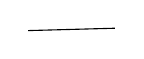
\begin{tikzpicture}\draw (0,0)--(1.1,0.03);\end{tikzpicture}}
\mspage{4}

\scanpage{6}
\mspage{\unsure{7|3}}
En résumé, on trouve

\uline{Prop.} Pour que $\Psi:W_{\mathrm{cof}}^{-1}C_{\mathrm{cof}}\longrightarrow W^{-1}C$ soit une équiv. de cat., il f. et s. que la condition suivante soit vérifiée :

$(\unsure{*})$ Pour \deleted{tout} diagramme
\diagram{\begin{tikzcd}x \arrow[r,shift left=.65ex,"\varphi"] \arrow[r,shift right=.65ex,"\psi"'] & y \arrow[r,"f","\sim"'] & y'\end{tikzcd}}
où $f\varphi=f\psi$, $f\in W$, $x,y\in C_{\mathrm{cof}}$ \inserted{(d'où $[\varphi]=[\psi]$ dans $W^{-1}C$)}, on a $[\varphi]=[\psi]$ dans $W_{\mathrm{cof}}^{-1}C_{\mathrm{cof}}$.

(condition impliquée par celle que $\Psi$ soit \uline{fidèle})

Nous allons travailler maintenant avec $C_{\mathrm{cof}}$ au lieu de $C$. -- donc quitte à changer de notations, on va supposer que tt objet de $C$ est cofibrant.

[\uline{NB} $C_{\mathrm{cof}}$ avec les notions induites par $W$ et cof est encore une catégorie \unsure{C1 : C3}], l'inclusion de $C_{\mathrm{cof}}$ dans $C$ commute aux sommes amalgamées \deleted{\unsure{qui}} relatives à des diagrammes
\diagram{\begin{tikzcd}a \arrow[r,"f"] \arrow[d,"g"'] & b\\ c &\end{tikzcd}}
tels que $f$ ou $g$ soit dans cof (les seules sommes dont on postule l'existence !).]

Soit, pour $x,y$ dans $C$,
\[
\uline{\mathrm{Ch}}_0(x,y)=\text{catégorie des diagrammes}
\]
\diagram{\begin{tikzcd}x \arrow[dr,"f"'] & y \arrow[d,"i","\sim"']\\ &\bar y\end{tikzcd}}
où $i\in W\cap\mathrm{cof}$ \deleted{\unsure{i.e.}} (\unsure{équi. faible couniverselle}\inserted{si $\mathrm{cof}=\mathrm{cof}_W$}). On définit des accouplements
\[
\uline{\mathrm{Ch}}_0(x,y)\times\uline{\mathrm{Ch}}_0(y,z)\longrightarrow\uline{\mathrm{Ch}}_0(x,z),\quad (F,G)\longmapsto G\mathbin{\cdot}F
\]
par
\diagram{\begin{tikzcd}
\unsure{x|a} \arrow[dr,"f"',"\deleted{\unsure{\varphi}}"] & y \arrow[d,hook,"i","\sim"'] \arrow[dr,"g"] & z \arrow[d,hook,"j","\sim"']\\
& \bar y \arrow[dr,"g'"',"\text{cocart}"] & \bar z \arrow[d,hook,"\unsure{k}","\sim"']\\
&&\bar z'
\end{tikzcd}}
\deleted{$\unsure{g'f}$}
\[
(g,j)\mathbin{\circ}(f,i)=(\unsure{g'g|g'f})\mathbin{\cdot}\unsure{kj}.
\]
\mspage{5}

\scanpage{7}
\figure{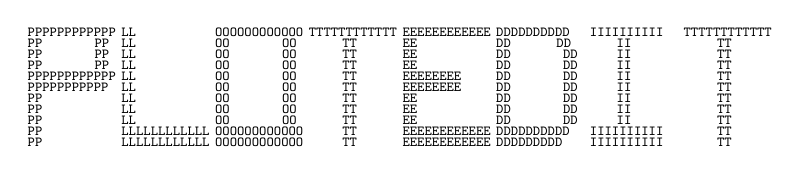
\begin{tikzpicture}[x=.085cm,y=.14cm]
\node[anchor=base west,inner sep=0pt,font=\tiny\ttfamily] at (0,0) {PPPPPPPPPPPP};
\node[anchor=base west,inner sep=0pt,font=\tiny\ttfamily] at (0,-1) {PP};
\node[anchor=base west,inner sep=0pt,font=\tiny\ttfamily] at (10,-1) {PP};
\node[anchor=base west,inner sep=0pt,font=\tiny\ttfamily] at (0,-2) {PP};
\node[anchor=base west,inner sep=0pt,font=\tiny\ttfamily] at (10,-2) {PP};
\node[anchor=base west,inner sep=0pt,font=\tiny\ttfamily] at (0,-3) {PP};
\node[anchor=base west,inner sep=0pt,font=\tiny\ttfamily] at (10,-3) {PP};
\node[anchor=base west,inner sep=0pt,font=\tiny\ttfamily] at (0,-4) {PPPPPPPPPPPP};
\node[anchor=base west,inner sep=0pt,font=\tiny\ttfamily] at (0,-5) {PPPPPPPPPPP};
\node[anchor=base west,inner sep=0pt,font=\tiny\ttfamily] at (0,-6) {PP};
\node[anchor=base west,inner sep=0pt,font=\tiny\ttfamily] at (0,-7) {PP};
\node[anchor=base west,inner sep=0pt,font=\tiny\ttfamily] at (0,-8) {PP};
\node[anchor=base west,inner sep=0pt,font=\tiny\ttfamily] at (0,-9) {PP};
\node[anchor=base west,inner sep=0pt,font=\tiny\ttfamily] at (0,-10) {PP};
\node[anchor=base west,inner sep=0pt,font=\tiny\ttfamily] at (14,0) {LL};
\node[anchor=base west,inner sep=0pt,font=\tiny\ttfamily] at (14,-1) {LL};
\node[anchor=base west,inner sep=0pt,font=\tiny\ttfamily] at (14,-2) {LL};
\node[anchor=base west,inner sep=0pt,font=\tiny\ttfamily] at (14,-3) {LL};
\node[anchor=base west,inner sep=0pt,font=\tiny\ttfamily] at (14,-4) {LL};
\node[anchor=base west,inner sep=0pt,font=\tiny\ttfamily] at (14,-5) {LL};
\node[anchor=base west,inner sep=0pt,font=\tiny\ttfamily] at (14,-6) {LL};
\node[anchor=base west,inner sep=0pt,font=\tiny\ttfamily] at (14,-7) {LL};
\node[anchor=base west,inner sep=0pt,font=\tiny\ttfamily] at (14,-8) {LL};
\node[anchor=base west,inner sep=0pt,font=\tiny\ttfamily] at (14,-9) {LLLLLLLLLLLL};
\node[anchor=base west,inner sep=0pt,font=\tiny\ttfamily] at (14,-10) {LLLLLLLLLLLL};
\node[anchor=base west,inner sep=0pt,font=\tiny\ttfamily] at (28,0) {OOOOOOOOOOOO};
\node[anchor=base west,inner sep=0pt,font=\tiny\ttfamily] at (28,-1) {OO};
\node[anchor=base west,inner sep=0pt,font=\tiny\ttfamily] at (38,-1) {OO};
\node[anchor=base west,inner sep=0pt,font=\tiny\ttfamily] at (28,-2) {OO};
\node[anchor=base west,inner sep=0pt,font=\tiny\ttfamily] at (38,-2) {OO};
\node[anchor=base west,inner sep=0pt,font=\tiny\ttfamily] at (28,-3) {OO};
\node[anchor=base west,inner sep=0pt,font=\tiny\ttfamily] at (38,-3) {OO};
\node[anchor=base west,inner sep=0pt,font=\tiny\ttfamily] at (28,-4) {OO};
\node[anchor=base west,inner sep=0pt,font=\tiny\ttfamily] at (38,-4) {OO};
\node[anchor=base west,inner sep=0pt,font=\tiny\ttfamily] at (28,-5) {OO};
\node[anchor=base west,inner sep=0pt,font=\tiny\ttfamily] at (38,-5) {OO};
\node[anchor=base west,inner sep=0pt,font=\tiny\ttfamily] at (28,-6) {OO};
\node[anchor=base west,inner sep=0pt,font=\tiny\ttfamily] at (38,-6) {OO};
\node[anchor=base west,inner sep=0pt,font=\tiny\ttfamily] at (28,-7) {OO};
\node[anchor=base west,inner sep=0pt,font=\tiny\ttfamily] at (38,-7) {OO};
\node[anchor=base west,inner sep=0pt,font=\tiny\ttfamily] at (28,-8) {OO};
\node[anchor=base west,inner sep=0pt,font=\tiny\ttfamily] at (38,-8) {OO};
\node[anchor=base west,inner sep=0pt,font=\tiny\ttfamily] at (28,-9) {OOOOOOOOOOOO};
\node[anchor=base west,inner sep=0pt,font=\tiny\ttfamily] at (28,-10) {OOOOOOOOOOOO};
\node[anchor=base west,inner sep=0pt,font=\tiny\ttfamily] at (42,0) {TTTTTTTTTTTT};
\node[anchor=base west,inner sep=0pt,font=\tiny\ttfamily] at (47,-1) {TT};
\node[anchor=base west,inner sep=0pt,font=\tiny\ttfamily] at (47,-2) {TT};
\node[anchor=base west,inner sep=0pt,font=\tiny\ttfamily] at (47,-3) {TT};
\node[anchor=base west,inner sep=0pt,font=\tiny\ttfamily] at (47,-4) {TT};
\node[anchor=base west,inner sep=0pt,font=\tiny\ttfamily] at (47,-5) {TT};
\node[anchor=base west,inner sep=0pt,font=\tiny\ttfamily] at (47,-6) {TT};
\node[anchor=base west,inner sep=0pt,font=\tiny\ttfamily] at (47,-7) {TT};
\node[anchor=base west,inner sep=0pt,font=\tiny\ttfamily] at (47,-8) {TT};
\node[anchor=base west,inner sep=0pt,font=\tiny\ttfamily] at (47,-9) {TT};
\node[anchor=base west,inner sep=0pt,font=\tiny\ttfamily] at (47,-10) {TT};
\node[anchor=base west,inner sep=0pt,font=\tiny\ttfamily] at (56,0) {EEEEEEEEEEEE};
\node[anchor=base west,inner sep=0pt,font=\tiny\ttfamily] at (56,-1) {EE};
\node[anchor=base west,inner sep=0pt,font=\tiny\ttfamily] at (56,-2) {EE};
\node[anchor=base west,inner sep=0pt,font=\tiny\ttfamily] at (56,-3) {EE};
\node[anchor=base west,inner sep=0pt,font=\tiny\ttfamily] at (56,-4) {EEEEEEEE};
\node[anchor=base west,inner sep=0pt,font=\tiny\ttfamily] at (56,-5) {EEEEEEEE};
\node[anchor=base west,inner sep=0pt,font=\tiny\ttfamily] at (56,-6) {EE};
\node[anchor=base west,inner sep=0pt,font=\tiny\ttfamily] at (56,-7) {EE};
\node[anchor=base west,inner sep=0pt,font=\tiny\ttfamily] at (56,-8) {EE};
\node[anchor=base west,inner sep=0pt,font=\tiny\ttfamily] at (56,-9) {EEEEEEEEEEEE};
\node[anchor=base west,inner sep=0pt,font=\tiny\ttfamily] at (56,-10) {EEEEEEEEEEEE};
\node[anchor=base west,inner sep=0pt,font=\tiny\ttfamily] at (70,0) {DDDDDDDDDD};
\node[anchor=base west,inner sep=0pt,font=\tiny\ttfamily] at (70,-1) {DD};
\node[anchor=base west,inner sep=0pt,font=\tiny\ttfamily] at (79,-1) {DD};
\node[anchor=base west,inner sep=0pt,font=\tiny\ttfamily] at (70,-2) {DD};
\node[anchor=base west,inner sep=0pt,font=\tiny\ttfamily] at (80,-2) {DD};
\node[anchor=base west,inner sep=0pt,font=\tiny\ttfamily] at (70,-3) {DD};
\node[anchor=base west,inner sep=0pt,font=\tiny\ttfamily] at (80,-3) {DD};
\node[anchor=base west,inner sep=0pt,font=\tiny\ttfamily] at (70,-4) {DD};
\node[anchor=base west,inner sep=0pt,font=\tiny\ttfamily] at (80,-4) {DD};
\node[anchor=base west,inner sep=0pt,font=\tiny\ttfamily] at (70,-5) {DD};
\node[anchor=base west,inner sep=0pt,font=\tiny\ttfamily] at (80,-5) {DD};
\node[anchor=base west,inner sep=0pt,font=\tiny\ttfamily] at (70,-6) {DD};
\node[anchor=base west,inner sep=0pt,font=\tiny\ttfamily] at (80,-6) {DD};
\node[anchor=base west,inner sep=0pt,font=\tiny\ttfamily] at (70,-7) {DD};
\node[anchor=base west,inner sep=0pt,font=\tiny\ttfamily] at (80,-7) {DD};
\node[anchor=base west,inner sep=0pt,font=\tiny\ttfamily] at (70,-8) {DD};
\node[anchor=base west,inner sep=0pt,font=\tiny\ttfamily] at (80,-8) {DD};
\node[anchor=base west,inner sep=0pt,font=\tiny\ttfamily] at (70,-9) {DDDDDDDDDD};
\node[anchor=base west,inner sep=0pt,font=\tiny\ttfamily] at (70,-10) {DDDDDDDDD};
\node[anchor=base west,inner sep=0pt,font=\tiny\ttfamily] at (84,0) {IIIIIIIIII};
\node[anchor=base west,inner sep=0pt,font=\tiny\ttfamily] at (88,-1) {II};
\node[anchor=base west,inner sep=0pt,font=\tiny\ttfamily] at (88,-2) {II};
\node[anchor=base west,inner sep=0pt,font=\tiny\ttfamily] at (88,-3) {II};
\node[anchor=base west,inner sep=0pt,font=\tiny\ttfamily] at (88,-4) {II};
\node[anchor=base west,inner sep=0pt,font=\tiny\ttfamily] at (88,-5) {II};
\node[anchor=base west,inner sep=0pt,font=\tiny\ttfamily] at (88,-6) {II};
\node[anchor=base west,inner sep=0pt,font=\tiny\ttfamily] at (88,-7) {II};
\node[anchor=base west,inner sep=0pt,font=\tiny\ttfamily] at (88,-8) {II};
\node[anchor=base west,inner sep=0pt,font=\tiny\ttfamily] at (84,-9) {IIIIIIIIII};
\node[anchor=base west,inner sep=0pt,font=\tiny\ttfamily] at (84,-10) {IIIIIIIIII};
\node[anchor=base west,inner sep=0pt,font=\tiny\ttfamily] at (98,0) {TTTTTTTTTTTT};
\node[anchor=base west,inner sep=0pt,font=\tiny\ttfamily] at (103,-1) {TT};
\node[anchor=base west,inner sep=0pt,font=\tiny\ttfamily] at (103,-2) {TT};
\node[anchor=base west,inner sep=0pt,font=\tiny\ttfamily] at (103,-3) {TT};
\node[anchor=base west,inner sep=0pt,font=\tiny\ttfamily] at (103,-4) {TT};
\node[anchor=base west,inner sep=0pt,font=\tiny\ttfamily] at (103,-5) {TT};
\node[anchor=base west,inner sep=0pt,font=\tiny\ttfamily] at (103,-6) {TT};
\node[anchor=base west,inner sep=0pt,font=\tiny\ttfamily] at (103,-7) {TT};
\node[anchor=base west,inner sep=0pt,font=\tiny\ttfamily] at (103,-8) {TT};
\node[anchor=base west,inner sep=0pt,font=\tiny\ttfamily] at (103,-9) {TT};
\node[anchor=base west,inner sep=0pt,font=\tiny\ttfamily] at (103,-10) {TT};
\end{tikzpicture}}

\texttt{****A\quad END\quad JOB 7747\quad PLOTEDIT\qquad ROOM\qquad 8.39.37 AM 25 AUG 82\quad R6.PR1\quad SYS JES2\quad JOB 7747\quad END\quad A****}

\texttt{****A\quad END\quad JOB 7747\quad PLOTEDIT\qquad ROOM\qquad 8.39.37 AM 25 AUG 82\quad R6.PR1\quad SYS JES2\quad JOB 7747\quad END\quad A****}

\texttt{****A\quad END\quad JOB 7747\quad PLOTEDIT\qquad ROOM\qquad 8.39.37 AM 25 AUG 82\quad R6.PR1\quad SYS JES2\quad JOB 7747\quad END\quad A****}

\texttt{****A\quad END\quad JOB 7747\quad PLOTEDIT\qquad ROOM\qquad 8.39.37 AM 25 AUG 82\quad R6.PR1\quad SYS JES2\quad JOB 7747\quad END\quad A****}

\texttt{****A\quad END\quad JOB 7747\quad PLOTEDIT\qquad ROOM\qquad 8.39.37 AM 25 AUG 82\quad R6.PR1\quad SYS JES2\quad JOB 7747\quad END\quad A****}

\texttt{****A\quad END\quad JOB 7747\quad PLOTEDIT\qquad ROOM\qquad 8.39.37 AM 25 AUG 82\quad R6.PR1\quad SYS JES2\quad JOB 7747\quad END\quad A****}

\mspage{6}

\scanpage{8}
\mspage{4)}
Cette composition est associative à iso can. près, et elle a des identités bilatères (\deleted{\unsure{par}} un iso can. !) savoir
\diagram{\begin{tikzcd}
x \arrow[dr,"1"'] & x \arrow[d,"1","\sim"'] \\
& x
\end{tikzcd}} noté $\uline{1}_x$.

On a d'autre part des \deleted{\unsure{appl.}} foncteurs
\[\operatorname{Hom}_C(x,y)_{\text{discret}}\longrightarrow\uline{\mathrm{Ch}}_0(x,y)\]
\deleted{\unsure{compatibles à}}
\[f\longmapsto(f,\operatorname{Id}_{\unsure{x|y}})\]
compatibles aux compositions. Ceci posé soit
\[\pi_0(x,y)\overset{\mathrm{def}}=\pi_0\uline{\mathrm{Ch}}_0(x,y);\]
alors la composition des $\uline{\mathrm{Ch}}_0$ définit une composition des $\pi_0(x,y)$, qui est associative (str. !) et admet les classes des $\uline{1}_x$ comme unités bilatères. D'où une catégorie, que je note $\widetilde C^{\unsure{2|?}}$, et un foncteur
\[C\longrightarrow\widetilde C.\]

Pour l'instant, on n'a utilisé rien sur $(C,W)$, [\deleted{\unsure{ni}} \unsure{ni} la donnée des $\mathrm{cof}\subset\mathrm{Fl}\,C$; \unsure{en se contentant} de prendre les flèches $i$ dans (\deleted{$\mathrm{cof}\cap W$}\inserted{$\unsure{\mathrm{Couniv.}W}$}) --- mais \deleted{\unsure{si}} on peut garder la construction, avec $\mathrm{cof}$ \inserted{\unsure{pas néc.}\ $=\mathrm{cof}_W$,} tel que $\mathrm{cof}\cap W\subset\deleted{\unsure{W}}\unsure{\mathrm{Couniv.}W}$]. \deleted{On} \inserted{Mais,} on veut prouver que ce foncteur transforme $f\in W$ en iso.
\diagram{\begin{tikzcd}
x \arrow[r,"f","\sim"'] & y \arrow[dr,"g?"'] & x \arrow[d,"i?","\sim"'] \\
&&\bar x
\end{tikzcd}}
on cherche $g,i$ tels que $(gf,i)\in\text{comp. conn. de }\uline{1}_x$ dans $\pi_0(\uline{\mathrm{Ch}}_0(x,x))$ et $(\bar f g,j)\in\text{comp. conn. de }\uline{1}_y$.
\diagram{\begin{tikzcd}
& x \arrow[r,"f","\sim"'] \arrow[d,"i","\sim"'] & y \arrow[d,"j"',"\sim"] \\
y \arrow[r,"g"'] & \bar x \arrow[r,"{\bar f\quad\sim}"',"\sim"] \arrow[ur,phantom,"(\text{cocart})" description] & \bar y
\end{tikzcd}}
\mspage{7}

\scanpage{9}
\figure{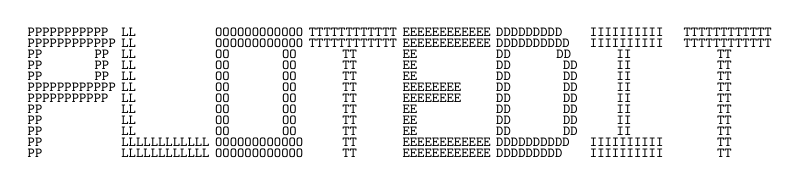
\begin{tikzpicture}[x=.085cm,y=.14cm]
\node[anchor=base west,inner sep=0pt,font=\tiny\ttfamily] at (0,0) {PPPPPPPPPPP};
\node[anchor=base west,inner sep=0pt,font=\tiny\ttfamily] at (0,-1) {PPPPPPPPPPPP};
\node[anchor=base west,inner sep=0pt,font=\tiny\ttfamily] at (0,-2) {PP};
\node[anchor=base west,inner sep=0pt,font=\tiny\ttfamily] at (10,-2) {PP};
\node[anchor=base west,inner sep=0pt,font=\tiny\ttfamily] at (0,-3) {PP};
\node[anchor=base west,inner sep=0pt,font=\tiny\ttfamily] at (10,-3) {PP};
\node[anchor=base west,inner sep=0pt,font=\tiny\ttfamily] at (0,-4) {PP};
\node[anchor=base west,inner sep=0pt,font=\tiny\ttfamily] at (10,-4) {PP};
\node[anchor=base west,inner sep=0pt,font=\tiny\ttfamily] at (0,-5) {PPPPPPPPPPPP};
\node[anchor=base west,inner sep=0pt,font=\tiny\ttfamily] at (0,-6) {PPPPPPPPPPP};
\node[anchor=base west,inner sep=0pt,font=\tiny\ttfamily] at (0,-7) {PP};
\node[anchor=base west,inner sep=0pt,font=\tiny\ttfamily] at (0,-8) {PP};
\node[anchor=base west,inner sep=0pt,font=\tiny\ttfamily] at (0,-9) {PP};
\node[anchor=base west,inner sep=0pt,font=\tiny\ttfamily] at (0,-10) {PP};
\node[anchor=base west,inner sep=0pt,font=\tiny\ttfamily] at (0,-11) {PP};
\node[anchor=base west,inner sep=0pt,font=\tiny\ttfamily] at (14,0) {LL};
\node[anchor=base west,inner sep=0pt,font=\tiny\ttfamily] at (14,-1) {LL};
\node[anchor=base west,inner sep=0pt,font=\tiny\ttfamily] at (14,-2) {LL};
\node[anchor=base west,inner sep=0pt,font=\tiny\ttfamily] at (14,-3) {LL};
\node[anchor=base west,inner sep=0pt,font=\tiny\ttfamily] at (14,-4) {LL};
\node[anchor=base west,inner sep=0pt,font=\tiny\ttfamily] at (14,-5) {LL};
\node[anchor=base west,inner sep=0pt,font=\tiny\ttfamily] at (14,-6) {LL};
\node[anchor=base west,inner sep=0pt,font=\tiny\ttfamily] at (14,-7) {LL};
\node[anchor=base west,inner sep=0pt,font=\tiny\ttfamily] at (14,-8) {LL};
\node[anchor=base west,inner sep=0pt,font=\tiny\ttfamily] at (14,-9) {LL};
\node[anchor=base west,inner sep=0pt,font=\tiny\ttfamily] at (14,-10) {LLLLLLLLLLLL};
\node[anchor=base west,inner sep=0pt,font=\tiny\ttfamily] at (14,-11) {LLLLLLLLLLLL};
\node[anchor=base west,inner sep=0pt,font=\tiny\ttfamily] at (28,0) {OOOOOOOOOOOO};
\node[anchor=base west,inner sep=0pt,font=\tiny\ttfamily] at (28,-1) {OOOOOOOOOOOO};
\node[anchor=base west,inner sep=0pt,font=\tiny\ttfamily] at (28,-2) {OO};
\node[anchor=base west,inner sep=0pt,font=\tiny\ttfamily] at (38,-2) {OO};
\node[anchor=base west,inner sep=0pt,font=\tiny\ttfamily] at (28,-3) {OO};
\node[anchor=base west,inner sep=0pt,font=\tiny\ttfamily] at (38,-3) {OO};
\node[anchor=base west,inner sep=0pt,font=\tiny\ttfamily] at (28,-4) {OO};
\node[anchor=base west,inner sep=0pt,font=\tiny\ttfamily] at (38,-4) {OO};
\node[anchor=base west,inner sep=0pt,font=\tiny\ttfamily] at (28,-5) {OO};
\node[anchor=base west,inner sep=0pt,font=\tiny\ttfamily] at (38,-5) {OO};
\node[anchor=base west,inner sep=0pt,font=\tiny\ttfamily] at (28,-6) {OO};
\node[anchor=base west,inner sep=0pt,font=\tiny\ttfamily] at (38,-6) {OO};
\node[anchor=base west,inner sep=0pt,font=\tiny\ttfamily] at (28,-7) {OO};
\node[anchor=base west,inner sep=0pt,font=\tiny\ttfamily] at (38,-7) {OO};
\node[anchor=base west,inner sep=0pt,font=\tiny\ttfamily] at (28,-8) {OO};
\node[anchor=base west,inner sep=0pt,font=\tiny\ttfamily] at (38,-8) {OO};
\node[anchor=base west,inner sep=0pt,font=\tiny\ttfamily] at (28,-9) {OO};
\node[anchor=base west,inner sep=0pt,font=\tiny\ttfamily] at (38,-9) {OO};
\node[anchor=base west,inner sep=0pt,font=\tiny\ttfamily] at (28,-10) {OOOOOOOOOOOO};
\node[anchor=base west,inner sep=0pt,font=\tiny\ttfamily] at (28,-11) {OOOOOOOOOOOO};
\node[anchor=base west,inner sep=0pt,font=\tiny\ttfamily] at (42,0) {TTTTTTTTTTTT};
\node[anchor=base west,inner sep=0pt,font=\tiny\ttfamily] at (42,-1) {TTTTTTTTTTTT};
\node[anchor=base west,inner sep=0pt,font=\tiny\ttfamily] at (47,-2) {TT};
\node[anchor=base west,inner sep=0pt,font=\tiny\ttfamily] at (47,-3) {TT};
\node[anchor=base west,inner sep=0pt,font=\tiny\ttfamily] at (47,-4) {TT};
\node[anchor=base west,inner sep=0pt,font=\tiny\ttfamily] at (47,-5) {TT};
\node[anchor=base west,inner sep=0pt,font=\tiny\ttfamily] at (47,-6) {TT};
\node[anchor=base west,inner sep=0pt,font=\tiny\ttfamily] at (47,-7) {TT};
\node[anchor=base west,inner sep=0pt,font=\tiny\ttfamily] at (47,-8) {TT};
\node[anchor=base west,inner sep=0pt,font=\tiny\ttfamily] at (47,-9) {TT};
\node[anchor=base west,inner sep=0pt,font=\tiny\ttfamily] at (47,-10) {TT};
\node[anchor=base west,inner sep=0pt,font=\tiny\ttfamily] at (47,-11) {TT};
\node[anchor=base west,inner sep=0pt,font=\tiny\ttfamily] at (56,0) {EEEEEEEEEEEE};
\node[anchor=base west,inner sep=0pt,font=\tiny\ttfamily] at (56,-1) {EEEEEEEEEEEE};
\node[anchor=base west,inner sep=0pt,font=\tiny\ttfamily] at (56,-2) {EE};
\node[anchor=base west,inner sep=0pt,font=\tiny\ttfamily] at (56,-3) {EE};
\node[anchor=base west,inner sep=0pt,font=\tiny\ttfamily] at (56,-4) {EE};
\node[anchor=base west,inner sep=0pt,font=\tiny\ttfamily] at (56,-5) {EEEEEEEE};
\node[anchor=base west,inner sep=0pt,font=\tiny\ttfamily] at (56,-6) {EEEEEEEE};
\node[anchor=base west,inner sep=0pt,font=\tiny\ttfamily] at (56,-7) {EE};
\node[anchor=base west,inner sep=0pt,font=\tiny\ttfamily] at (56,-8) {EE};
\node[anchor=base west,inner sep=0pt,font=\tiny\ttfamily] at (56,-9) {EE};
\node[anchor=base west,inner sep=0pt,font=\tiny\ttfamily] at (56,-10) {EEEEEEEEEEEE};
\node[anchor=base west,inner sep=0pt,font=\tiny\ttfamily] at (56,-11) {EEEEEEEEEEEE};
\node[anchor=base west,inner sep=0pt,font=\tiny\ttfamily] at (70,0) {DDDDDDDDD};
\node[anchor=base west,inner sep=0pt,font=\tiny\ttfamily] at (70,-1) {DDDDDDDDDD};
\node[anchor=base west,inner sep=0pt,font=\tiny\ttfamily] at (70,-2) {DD};
\node[anchor=base west,inner sep=0pt,font=\tiny\ttfamily] at (79,-2) {DD};
\node[anchor=base west,inner sep=0pt,font=\tiny\ttfamily] at (70,-3) {DD};
\node[anchor=base west,inner sep=0pt,font=\tiny\ttfamily] at (80,-3) {DD};
\node[anchor=base west,inner sep=0pt,font=\tiny\ttfamily] at (70,-4) {DD};
\node[anchor=base west,inner sep=0pt,font=\tiny\ttfamily] at (80,-4) {DD};
\node[anchor=base west,inner sep=0pt,font=\tiny\ttfamily] at (70,-5) {DD};
\node[anchor=base west,inner sep=0pt,font=\tiny\ttfamily] at (80,-5) {DD};
\node[anchor=base west,inner sep=0pt,font=\tiny\ttfamily] at (70,-6) {DD};
\node[anchor=base west,inner sep=0pt,font=\tiny\ttfamily] at (80,-6) {DD};
\node[anchor=base west,inner sep=0pt,font=\tiny\ttfamily] at (70,-7) {DD};
\node[anchor=base west,inner sep=0pt,font=\tiny\ttfamily] at (80,-7) {DD};
\node[anchor=base west,inner sep=0pt,font=\tiny\ttfamily] at (70,-8) {DD};
\node[anchor=base west,inner sep=0pt,font=\tiny\ttfamily] at (80,-8) {DD};
\node[anchor=base west,inner sep=0pt,font=\tiny\ttfamily] at (70,-9) {DD};
\node[anchor=base west,inner sep=0pt,font=\tiny\ttfamily] at (80,-9) {DD};
\node[anchor=base west,inner sep=0pt,font=\tiny\ttfamily] at (70,-10) {DDDDDDDDDD};
\node[anchor=base west,inner sep=0pt,font=\tiny\ttfamily] at (70,-11) {DDDDDDDDD};
\node[anchor=base west,inner sep=0pt,font=\tiny\ttfamily] at (84,0) {IIIIIIIIII};
\node[anchor=base west,inner sep=0pt,font=\tiny\ttfamily] at (84,-1) {IIIIIIIIII};
\node[anchor=base west,inner sep=0pt,font=\tiny\ttfamily] at (88,-2) {II};
\node[anchor=base west,inner sep=0pt,font=\tiny\ttfamily] at (88,-3) {II};
\node[anchor=base west,inner sep=0pt,font=\tiny\ttfamily] at (88,-4) {II};
\node[anchor=base west,inner sep=0pt,font=\tiny\ttfamily] at (88,-5) {II};
\node[anchor=base west,inner sep=0pt,font=\tiny\ttfamily] at (88,-6) {II};
\node[anchor=base west,inner sep=0pt,font=\tiny\ttfamily] at (88,-7) {II};
\node[anchor=base west,inner sep=0pt,font=\tiny\ttfamily] at (88,-8) {II};
\node[anchor=base west,inner sep=0pt,font=\tiny\ttfamily] at (88,-9) {II};
\node[anchor=base west,inner sep=0pt,font=\tiny\ttfamily] at (84,-10) {IIIIIIIIII};
\node[anchor=base west,inner sep=0pt,font=\tiny\ttfamily] at (84,-11) {IIIIIIIIII};
\node[anchor=base west,inner sep=0pt,font=\tiny\ttfamily] at (98,0) {TTTTTTTTTTTT};
\node[anchor=base west,inner sep=0pt,font=\tiny\ttfamily] at (98,-1) {TTTTTTTTTTTT};
\node[anchor=base west,inner sep=0pt,font=\tiny\ttfamily] at (103,-2) {TT};
\node[anchor=base west,inner sep=0pt,font=\tiny\ttfamily] at (103,-3) {TT};
\node[anchor=base west,inner sep=0pt,font=\tiny\ttfamily] at (103,-4) {TT};
\node[anchor=base west,inner sep=0pt,font=\tiny\ttfamily] at (103,-5) {TT};
\node[anchor=base west,inner sep=0pt,font=\tiny\ttfamily] at (103,-6) {TT};
\node[anchor=base west,inner sep=0pt,font=\tiny\ttfamily] at (103,-7) {TT};
\node[anchor=base west,inner sep=0pt,font=\tiny\ttfamily] at (103,-8) {TT};
\node[anchor=base west,inner sep=0pt,font=\tiny\ttfamily] at (103,-9) {TT};
\node[anchor=base west,inner sep=0pt,font=\tiny\ttfamily] at (103,-10) {TT};
\node[anchor=base west,inner sep=0pt,font=\tiny\ttfamily] at (103,-11) {TT};
\end{tikzpicture}}
\margin{\unsure{P|9}}
\texttt{****A\quad START\quad JOB 7747\quad PLOTEDIT\qquad ROOM\qquad 8.39.24 AM 25 AUG 82\quad R6.PR1\quad SYS JES2\quad JOB 7747\quad START\quad A****}

\texttt{****A\quad START\quad JOB 7747\quad PLOTEDIT\qquad ROOM\qquad 8.39.24 AM 25 AUG 82\quad R6.PR1\quad SYS JES2\quad JOB 7747\quad START\quad A****}

\texttt{****A\quad START\quad JOB 7747\quad PLOTEDIT\qquad ROOM\qquad 8.39.24 AM 25 AUG 82\quad R6.PR1\quad SYS JES2\quad JOB 7747\quad START\quad A****}

\texttt{****A\quad START\quad JOB 7747\quad PLOTEDIT\qquad ROOM\qquad 8.39.24 AM 25 AUG 82\quad R6.PR1\quad SYS JES2\quad JOB 7747\quad START\quad A****}

\texttt{****A\quad START\quad JOB 7747\quad PLOTEDIT\qquad ROOM\qquad 8.39.24 AM 25 AUG 82\quad R6.PR1\quad SYS JES2\quad JOB 7747\quad START\quad A****}

\texttt{****A\quad START\quad JOB 7747\quad PLOTEDIT\qquad ROOM\qquad 8.39.24 AM 25 AUG 82\quad R6.PR1\quad SYS JES2\quad JOB 7747\quad START\quad A****}

\texttt{DERNIERE MISE A JOUR DE JOURNAL : 11-08-82}

\diagram{\begin{array}{ll|ll}
\text{CRAY 1}&579/1&\unsure{849}&\text{CRAY 1}\\
\text{GRAPHI1}&2&&
\end{array}}

\texttt{TRACEUR I\quad BUFFER 1020\quad BANDE 9 PISTES\quad PLUMES : 3\quad XMAX = 10100.0\quad YMAX = 30.0\quad STNB = 100.00000}

\texttt{25/ 8/ 82\qquad 8 HEURES 37 MINUTES}

\diagram{\begin{array}{lll}
\texttt{JOB}&\texttt{BANDE IBM NUMERO}&\texttt{TRACEUR UTILISE}\\
&\texttt{****************************************}&\texttt{REMISE DE LA BANDE}\\
&&\texttt{DEBUT DE TRAITEMENT}\\
&&\texttt{FIN DE TRAITEMENT}\\
&&\texttt{REMISE DES GRAPH.}\\
&&\texttt{INCIDENTS SURVENUS}
\end{array}}

\diagram{\begin{array}{lllllllll}
\texttt{PLOT 3C}&&\texttt{CALQUE}&&&&0&0&\\
\texttt{CNU*0579 GRAPHI1}&&&\texttt{I.C}&82237&083702&0&0&\\
\texttt{GRAPHI1}&\texttt{CNU*0579}&82237&\texttt{M06}&\texttt{P02900500}&7\quad0&0&0&3
\end{array}}
\mspage{8}

\scanpage{10}
\mspage{5)}
\margin{\uline{NB} On utilise $y\in\mathrm{Cof}$ $\longleftarrow$ ici}
On utilise le weak lifting \unsure{lemme|lemma} pour
\diagram{\begin{tikzcd}
\varnothing \arrow[r] \arrow[d] & x \arrow[d,"f","\sim"'] \arrow[r,dashed,hook,"i","\sim"'] & \bar x \arrow[dl,dashed,"\alpha\ \deleted{\unsure{\varphi}}","\sim"'] \\
y \arrow[r,"1"] & y \arrow[ur,dashed,bend right=45,"g"'] & {}
\end{tikzcd}}
donc il existe $i,\alpha$ avec $\alpha i=f$, \deleted{\unsure{et}} $i\in W\cap\mathrm{cof}$, et $\alpha$ admet une section $g$
\[\alpha g=1_y\]
Je dis que $(g,i)$ est l'inverse \inserted{cherché.} \deleted{$\unsure{\alpha g=\operatorname{id}_y}$}
\deleted{Considérons alors}

Pour $(gf,i)\sim\uline{1}_x$, on a envie d'utiliser le diagramme commutatif ci-contre, le seul ennui c'est que, on a $\alpha\in W$ mais pas néc. $\alpha\in\mathrm{cof}$, donc $\alpha i\ (=f)$ pas néc. dans \deleted{\unsure{W}} $\mathrm{cof}$ (alors qu'il est dans $W$).
\diagram{\begin{tikzcd}[column sep=large,row sep=small]
x \arrow[dd,"1_x"'] \arrow[dr,"gf"] \arrow[dddrr,dashed,"f" near end] & & x \arrow[dl,"i","\sim"'] \arrow[ddll,"1_x","\sim"'] \\
&\bar x \arrow[ddr,dashed,"\alpha","\sim"']&\\
x \arrow[drr,dashed,"f"'] & \deleted{\unsure{f}} &\\
&& y
\end{tikzcd}}
Ça marcherait si on pouvait trouver $y\xrightarrow[\sim]{\beta}y'$ \inserted{dans $W$,} tel que le composé $\beta f$ soit non seulement dans $W$, mais de plus, dans $\mathrm{cof}$.

Visiblement, ce n'est pas \unsure{tjs} le cas (prendre le cas où les $\mathrm{cof}$ sont les monos, et où $f$ n'est \uline{pas} un mono !). Ça se présente mal !
\diagram{\begin{tikzcd}
x \arrow[d,"f"'] \arrow[dr] &\\
y \arrow[r,"\beta"']&y'
\end{tikzcd}}
On va donc plutôt définir d'abord le foncteur canonique
\[\widetilde C\longrightarrow W^{-1}C\]
\[\unsure{\Phi|\varphi}:\quad x\longmapsto x\]
\[(f,i)\longmapsto[i]^{-1}[f]\]
il est immédiat que c'est compatible avec les identités et la composition. Donc on a bien foncteur \deleted{\unsure{injectif}} \inserted{bijectif} sur objets. Je dis que c'est surjectif sur les flèches; Il suffit de voir, par composition, que si $f:x\longrightarrow y$ est dans $W$, alors $[f]^{-1}$ provient de $\widetilde C$. On va prendre \deleted{$(y,x)$} $y\longrightarrow x$ dans $\widetilde C$, défini par $(g,i)$, \deleted{\unsure{À priori que}} $[i]^{-1}[g]$, pour prouver que $[i]^{-1}[g]=[f]^{-1}$, il suffit de prouver que $[f][i]^{-1}[g]=[\uline{1}_y]$, or $\alpha i=f$ entraîne $[\alpha][i]=[f]$ donc $[f][i]^{-1}=[\alpha]$, donc le \unsure{produit} est $[\alpha][g]=[\alpha g]=[1_y]$, OK.
\mspage{9}

\scanpage{11}
\texttt{//*\quad PLOTEDIT7747\qquad I}

\figure{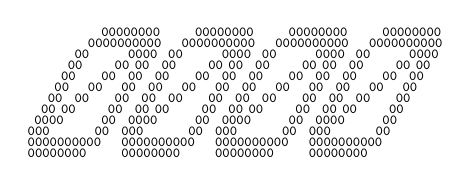
\begin{tikzpicture}[x=.085cm,y=.14cm]
\node[anchor=base west,inner sep=0pt,font=\tiny\ttfamily] at (11,0) {00000000};
\node[anchor=base west,inner sep=0pt,font=\tiny\ttfamily] at (9,-1) {0000000000};
\node[anchor=base west,inner sep=0pt,font=\tiny\ttfamily] at (7,-2) {00};
\node[anchor=base west,inner sep=0pt,font=\tiny\ttfamily] at (15,-2) {0000};
\node[anchor=base west,inner sep=0pt,font=\tiny\ttfamily] at (6,-3) {00};
\node[anchor=base west,inner sep=0pt,font=\tiny\ttfamily] at (13,-3) {00};
\node[anchor=base west,inner sep=0pt,font=\tiny\ttfamily] at (16,-3) {00};
\node[anchor=base west,inner sep=0pt,font=\tiny\ttfamily] at (5,-4) {00};
\node[anchor=base west,inner sep=0pt,font=\tiny\ttfamily] at (11,-4) {00};
\node[anchor=base west,inner sep=0pt,font=\tiny\ttfamily] at (15,-4) {00};
\node[anchor=base west,inner sep=0pt,font=\tiny\ttfamily] at (4,-5) {00};
\node[anchor=base west,inner sep=0pt,font=\tiny\ttfamily] at (9,-5) {00};
\node[anchor=base west,inner sep=0pt,font=\tiny\ttfamily] at (14,-5) {00};
\node[anchor=base west,inner sep=0pt,font=\tiny\ttfamily] at (3,-6) {00};
\node[anchor=base west,inner sep=0pt,font=\tiny\ttfamily] at (7,-6) {00};
\node[anchor=base west,inner sep=0pt,font=\tiny\ttfamily] at (13,-6) {00};
\node[anchor=base west,inner sep=0pt,font=\tiny\ttfamily] at (2,-7) {00};
\node[anchor=base west,inner sep=0pt,font=\tiny\ttfamily] at (5,-7) {00};
\node[anchor=base west,inner sep=0pt,font=\tiny\ttfamily] at (12,-7) {00};
\node[anchor=base west,inner sep=0pt,font=\tiny\ttfamily] at (1,-8) {0000};
\node[anchor=base west,inner sep=0pt,font=\tiny\ttfamily] at (11,-8) {00};
\node[anchor=base west,inner sep=0pt,font=\tiny\ttfamily] at (0,-9) {000};
\node[anchor=base west,inner sep=0pt,font=\tiny\ttfamily] at (10,-9) {00};
\node[anchor=base west,inner sep=0pt,font=\tiny\ttfamily] at (0,-10) {0000000000};
\node[anchor=base west,inner sep=0pt,font=\tiny\ttfamily] at (0,-11) {00000000};
\node[anchor=base west,inner sep=0pt,font=\tiny\ttfamily] at (25,0) {00000000};
\node[anchor=base west,inner sep=0pt,font=\tiny\ttfamily] at (23,-1) {0000000000};
\node[anchor=base west,inner sep=0pt,font=\tiny\ttfamily] at (21,-2) {00};
\node[anchor=base west,inner sep=0pt,font=\tiny\ttfamily] at (29,-2) {0000};
\node[anchor=base west,inner sep=0pt,font=\tiny\ttfamily] at (20,-3) {00};
\node[anchor=base west,inner sep=0pt,font=\tiny\ttfamily] at (27,-3) {00};
\node[anchor=base west,inner sep=0pt,font=\tiny\ttfamily] at (30,-3) {00};
\node[anchor=base west,inner sep=0pt,font=\tiny\ttfamily] at (19,-4) {00};
\node[anchor=base west,inner sep=0pt,font=\tiny\ttfamily] at (25,-4) {00};
\node[anchor=base west,inner sep=0pt,font=\tiny\ttfamily] at (29,-4) {00};
\node[anchor=base west,inner sep=0pt,font=\tiny\ttfamily] at (18,-5) {00};
\node[anchor=base west,inner sep=0pt,font=\tiny\ttfamily] at (23,-5) {00};
\node[anchor=base west,inner sep=0pt,font=\tiny\ttfamily] at (28,-5) {00};
\node[anchor=base west,inner sep=0pt,font=\tiny\ttfamily] at (17,-6) {00};
\node[anchor=base west,inner sep=0pt,font=\tiny\ttfamily] at (21,-6) {00};
\node[anchor=base west,inner sep=0pt,font=\tiny\ttfamily] at (27,-6) {00};
\node[anchor=base west,inner sep=0pt,font=\tiny\ttfamily] at (16,-7) {00};
\node[anchor=base west,inner sep=0pt,font=\tiny\ttfamily] at (19,-7) {00};
\node[anchor=base west,inner sep=0pt,font=\tiny\ttfamily] at (26,-7) {00};
\node[anchor=base west,inner sep=0pt,font=\tiny\ttfamily] at (15,-8) {0000};
\node[anchor=base west,inner sep=0pt,font=\tiny\ttfamily] at (25,-8) {00};
\node[anchor=base west,inner sep=0pt,font=\tiny\ttfamily] at (14,-9) {000};
\node[anchor=base west,inner sep=0pt,font=\tiny\ttfamily] at (24,-9) {00};
\node[anchor=base west,inner sep=0pt,font=\tiny\ttfamily] at (14,-10) {0000000000};
\node[anchor=base west,inner sep=0pt,font=\tiny\ttfamily] at (14,-11) {00000000};
\node[anchor=base west,inner sep=0pt,font=\tiny\ttfamily] at (39,0) {00000000};
\node[anchor=base west,inner sep=0pt,font=\tiny\ttfamily] at (37,-1) {0000000000};
\node[anchor=base west,inner sep=0pt,font=\tiny\ttfamily] at (35,-2) {00};
\node[anchor=base west,inner sep=0pt,font=\tiny\ttfamily] at (43,-2) {0000};
\node[anchor=base west,inner sep=0pt,font=\tiny\ttfamily] at (34,-3) {00};
\node[anchor=base west,inner sep=0pt,font=\tiny\ttfamily] at (41,-3) {00};
\node[anchor=base west,inner sep=0pt,font=\tiny\ttfamily] at (44,-3) {00};
\node[anchor=base west,inner sep=0pt,font=\tiny\ttfamily] at (33,-4) {00};
\node[anchor=base west,inner sep=0pt,font=\tiny\ttfamily] at (39,-4) {00};
\node[anchor=base west,inner sep=0pt,font=\tiny\ttfamily] at (43,-4) {00};
\node[anchor=base west,inner sep=0pt,font=\tiny\ttfamily] at (32,-5) {00};
\node[anchor=base west,inner sep=0pt,font=\tiny\ttfamily] at (37,-5) {00};
\node[anchor=base west,inner sep=0pt,font=\tiny\ttfamily] at (42,-5) {00};
\node[anchor=base west,inner sep=0pt,font=\tiny\ttfamily] at (31,-6) {00};
\node[anchor=base west,inner sep=0pt,font=\tiny\ttfamily] at (35,-6) {00};
\node[anchor=base west,inner sep=0pt,font=\tiny\ttfamily] at (41,-6) {00};
\node[anchor=base west,inner sep=0pt,font=\tiny\ttfamily] at (30,-7) {00};
\node[anchor=base west,inner sep=0pt,font=\tiny\ttfamily] at (33,-7) {00};
\node[anchor=base west,inner sep=0pt,font=\tiny\ttfamily] at (40,-7) {00};
\node[anchor=base west,inner sep=0pt,font=\tiny\ttfamily] at (29,-8) {0000};
\node[anchor=base west,inner sep=0pt,font=\tiny\ttfamily] at (39,-8) {00};
\node[anchor=base west,inner sep=0pt,font=\tiny\ttfamily] at (28,-9) {000};
\node[anchor=base west,inner sep=0pt,font=\tiny\ttfamily] at (38,-9) {00};
\node[anchor=base west,inner sep=0pt,font=\tiny\ttfamily] at (28,-10) {0000000000};
\node[anchor=base west,inner sep=0pt,font=\tiny\ttfamily] at (28,-11) {00000000};
\node[anchor=base west,inner sep=0pt,font=\tiny\ttfamily] at (53,0) {00000000};
\node[anchor=base west,inner sep=0pt,font=\tiny\ttfamily] at (51,-1) {0000000000};
\node[anchor=base west,inner sep=0pt,font=\tiny\ttfamily] at (49,-2) {00};
\node[anchor=base west,inner sep=0pt,font=\tiny\ttfamily] at (57,-2) {0000};
\node[anchor=base west,inner sep=0pt,font=\tiny\ttfamily] at (48,-3) {00};
\node[anchor=base west,inner sep=0pt,font=\tiny\ttfamily] at (55,-3) {00};
\node[anchor=base west,inner sep=0pt,font=\tiny\ttfamily] at (58,-3) {00};
\node[anchor=base west,inner sep=0pt,font=\tiny\ttfamily] at (47,-4) {00};
\node[anchor=base west,inner sep=0pt,font=\tiny\ttfamily] at (53,-4) {00};
\node[anchor=base west,inner sep=0pt,font=\tiny\ttfamily] at (57,-4) {00};
\node[anchor=base west,inner sep=0pt,font=\tiny\ttfamily] at (46,-5) {00};
\node[anchor=base west,inner sep=0pt,font=\tiny\ttfamily] at (51,-5) {00};
\node[anchor=base west,inner sep=0pt,font=\tiny\ttfamily] at (56,-5) {00};
\node[anchor=base west,inner sep=0pt,font=\tiny\ttfamily] at (45,-6) {00};
\node[anchor=base west,inner sep=0pt,font=\tiny\ttfamily] at (49,-6) {00};
\node[anchor=base west,inner sep=0pt,font=\tiny\ttfamily] at (55,-6) {00};
\node[anchor=base west,inner sep=0pt,font=\tiny\ttfamily] at (44,-7) {00};
\node[anchor=base west,inner sep=0pt,font=\tiny\ttfamily] at (47,-7) {00};
\node[anchor=base west,inner sep=0pt,font=\tiny\ttfamily] at (54,-7) {00};
\node[anchor=base west,inner sep=0pt,font=\tiny\ttfamily] at (43,-8) {0000};
\node[anchor=base west,inner sep=0pt,font=\tiny\ttfamily] at (53,-8) {00};
\node[anchor=base west,inner sep=0pt,font=\tiny\ttfamily] at (42,-9) {000};
\node[anchor=base west,inner sep=0pt,font=\tiny\ttfamily] at (52,-9) {00};
\node[anchor=base west,inner sep=0pt,font=\tiny\ttfamily] at (42,-10) {0000000000};
\node[anchor=base west,inner sep=0pt,font=\tiny\ttfamily] at (42,-11) {00000000};
\end{tikzpicture}}

\figure{
\begin{tikzpicture}[x=.085cm,y=.14cm]
\node[anchor=base west,inner sep=0pt,font=\tiny\ttfamily] at (0,0) {PPPPPPPPPPP};
\node[anchor=base west,inner sep=0pt,font=\tiny\ttfamily] at (14,0) {LL};
\node[anchor=base west,inner sep=0pt,font=\tiny\ttfamily] at (28,0) {OOOOOOOOOOOO};
\node[anchor=base west,inner sep=0pt,font=\tiny\ttfamily] at (42,0) {TTTTTTTTTTTT};
\node[anchor=base west,inner sep=0pt,font=\tiny\ttfamily] at (56,0) {EEEEEEEEEEEE};
\node[anchor=base west,inner sep=0pt,font=\tiny\ttfamily] at (70,0) {DDDDDDDDD};
\node[anchor=base west,inner sep=0pt,font=\tiny\ttfamily] at (84,0) {IIIIIIIIII};
\node[anchor=base west,inner sep=0pt,font=\tiny\ttfamily] at (98,0) {TTTTTTTTTTTT};
\end{tikzpicture}}

\mspage{10}

\scanpage{12}
\mspage{6)}
La difficulté, c'est qu'il n'est pas clair que le foncteur
\[\widetilde C\longrightarrow W^{-1}C\]
précédent soit aussi \uline{fidèle} (ce qui impliquerait que c'est une équivalence des catégories \inserted{et même un iso}). \deleted{Dans ce cas \unsure{le foncteur inverse serait forcément donné par}} \inserted{Il revient au $=$ de dire} que le foncteur can $C\mathbin{-}\widetilde C$ (dont le composé avec $\widetilde C\mathbin{-}W^{-1}C$ est bien le foncteur can. $C\mathbin{-}W^{-1}C$) transforme flèches de $W$ en iso, ou encore que la construction qu'on vient d'\unsure{envisager}, pour \deleted{le cas} \inserted{trouver} un inverse de $[f,i]$ dans $\widetilde C$, est bien valable, \deleted{\unsure{ce que}}
Cela \unsure{entraînerait} d'ailleurs \inserted{semble-t-il,} que, \deleted{le} posant $W_0=W\cap\mathrm{cof}$, le foncteur
\[W_0^{-1}C\longrightarrow W^{-1}C\]
serait une équivalence de catégories, car
\[\widetilde C\longrightarrow W^{-1}C\]
se factorise visiblement par
\diagram{\begin{tikzcd}
\widetilde C \arrow[r] \arrow[d,phantom,"\unsure{\simeq}"] & W_0^{-1}C \arrow[r]& W^{-1}C\\
W^{-1}C&&
\end{tikzcd}}
Mais je doute qu'il suffise d'inverser les équiv. faibles \uline{cofibrantes}, pour que \unsure{ttes} les équiv. faibles deviennent inversibles !

Je rectifie donc le tir, en prenant plutôt la catégorie (notée maintenant par $\widetilde C$) ayant $\unsure{=^{\mathrm{s}}}$ objets que $C$, \deleted{\unsure{et définie ainsi par les flèches de $x\longrightarrow y$}} \inserted{et \unsure{ayant pour} les $\pi_0$ des $\uline{\mathrm{Ch}}_0(x,y)$,} \deleted{\unsure{définie maintenant}} \inserted{cette catégorie} (pour $x,y$ donnés) comme celle des diagrammes
\diagram{\begin{tikzcd}
\deleted{\unsure{x}} \arrow[r,phantom,"\deleted{\unsure{\longrightarrow}}"]&\deleted{\unsure{y}}
\end{tikzcd}}
\diagram{\begin{tikzcd}
x \arrow[dr,hook,"f"']&y\arrow[d,"i"',"\sim"]\\
&\bar y
\end{tikzcd}}
avec $\left\{\begin{array}{l}f\in\mathrm{cof}\\i\in W\end{array}\right.$
\mspage{11}

\scanpage{13}
\texttt{//*\quad DOCUGRA20005\qquad I}

\figure{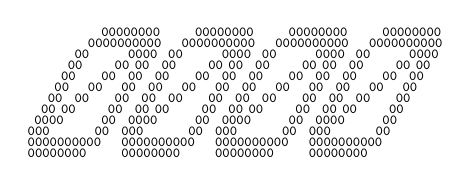
\begin{tikzpicture}[x=.085cm,y=.14cm]
\node[anchor=base west,inner sep=0pt,font=\tiny\ttfamily] at (11,0) {00000000};
\node[anchor=base west,inner sep=0pt,font=\tiny\ttfamily] at (9,-1) {0000000000};
\node[anchor=base west,inner sep=0pt,font=\tiny\ttfamily] at (7,-2) {00};
\node[anchor=base west,inner sep=0pt,font=\tiny\ttfamily] at (15,-2) {0000};
\node[anchor=base west,inner sep=0pt,font=\tiny\ttfamily] at (6,-3) {00};
\node[anchor=base west,inner sep=0pt,font=\tiny\ttfamily] at (13,-3) {00};
\node[anchor=base west,inner sep=0pt,font=\tiny\ttfamily] at (16,-3) {00};
\node[anchor=base west,inner sep=0pt,font=\tiny\ttfamily] at (5,-4) {00};
\node[anchor=base west,inner sep=0pt,font=\tiny\ttfamily] at (11,-4) {00};
\node[anchor=base west,inner sep=0pt,font=\tiny\ttfamily] at (15,-4) {00};
\node[anchor=base west,inner sep=0pt,font=\tiny\ttfamily] at (4,-5) {00};
\node[anchor=base west,inner sep=0pt,font=\tiny\ttfamily] at (9,-5) {00};
\node[anchor=base west,inner sep=0pt,font=\tiny\ttfamily] at (14,-5) {00};
\node[anchor=base west,inner sep=0pt,font=\tiny\ttfamily] at (3,-6) {00};
\node[anchor=base west,inner sep=0pt,font=\tiny\ttfamily] at (7,-6) {00};
\node[anchor=base west,inner sep=0pt,font=\tiny\ttfamily] at (13,-6) {00};
\node[anchor=base west,inner sep=0pt,font=\tiny\ttfamily] at (2,-7) {00};
\node[anchor=base west,inner sep=0pt,font=\tiny\ttfamily] at (5,-7) {00};
\node[anchor=base west,inner sep=0pt,font=\tiny\ttfamily] at (12,-7) {00};
\node[anchor=base west,inner sep=0pt,font=\tiny\ttfamily] at (1,-8) {0000};
\node[anchor=base west,inner sep=0pt,font=\tiny\ttfamily] at (11,-8) {00};
\node[anchor=base west,inner sep=0pt,font=\tiny\ttfamily] at (0,-9) {000};
\node[anchor=base west,inner sep=0pt,font=\tiny\ttfamily] at (10,-9) {00};
\node[anchor=base west,inner sep=0pt,font=\tiny\ttfamily] at (0,-10) {0000000000};
\node[anchor=base west,inner sep=0pt,font=\tiny\ttfamily] at (0,-11) {00000000};
\node[anchor=base west,inner sep=0pt,font=\tiny\ttfamily] at (25,0) {00000000};
\node[anchor=base west,inner sep=0pt,font=\tiny\ttfamily] at (23,-1) {0000000000};
\node[anchor=base west,inner sep=0pt,font=\tiny\ttfamily] at (21,-2) {00};
\node[anchor=base west,inner sep=0pt,font=\tiny\ttfamily] at (29,-2) {0000};
\node[anchor=base west,inner sep=0pt,font=\tiny\ttfamily] at (20,-3) {00};
\node[anchor=base west,inner sep=0pt,font=\tiny\ttfamily] at (27,-3) {00};
\node[anchor=base west,inner sep=0pt,font=\tiny\ttfamily] at (30,-3) {00};
\node[anchor=base west,inner sep=0pt,font=\tiny\ttfamily] at (19,-4) {00};
\node[anchor=base west,inner sep=0pt,font=\tiny\ttfamily] at (25,-4) {00};
\node[anchor=base west,inner sep=0pt,font=\tiny\ttfamily] at (29,-4) {00};
\node[anchor=base west,inner sep=0pt,font=\tiny\ttfamily] at (18,-5) {00};
\node[anchor=base west,inner sep=0pt,font=\tiny\ttfamily] at (23,-5) {00};
\node[anchor=base west,inner sep=0pt,font=\tiny\ttfamily] at (28,-5) {00};
\node[anchor=base west,inner sep=0pt,font=\tiny\ttfamily] at (17,-6) {00};
\node[anchor=base west,inner sep=0pt,font=\tiny\ttfamily] at (21,-6) {00};
\node[anchor=base west,inner sep=0pt,font=\tiny\ttfamily] at (27,-6) {00};
\node[anchor=base west,inner sep=0pt,font=\tiny\ttfamily] at (16,-7) {00};
\node[anchor=base west,inner sep=0pt,font=\tiny\ttfamily] at (19,-7) {00};
\node[anchor=base west,inner sep=0pt,font=\tiny\ttfamily] at (26,-7) {00};
\node[anchor=base west,inner sep=0pt,font=\tiny\ttfamily] at (15,-8) {0000};
\node[anchor=base west,inner sep=0pt,font=\tiny\ttfamily] at (25,-8) {00};
\node[anchor=base west,inner sep=0pt,font=\tiny\ttfamily] at (14,-9) {000};
\node[anchor=base west,inner sep=0pt,font=\tiny\ttfamily] at (24,-9) {00};
\node[anchor=base west,inner sep=0pt,font=\tiny\ttfamily] at (14,-10) {0000000000};
\node[anchor=base west,inner sep=0pt,font=\tiny\ttfamily] at (14,-11) {00000000};
\node[anchor=base west,inner sep=0pt,font=\tiny\ttfamily] at (39,0) {00000000};
\node[anchor=base west,inner sep=0pt,font=\tiny\ttfamily] at (37,-1) {0000000000};
\node[anchor=base west,inner sep=0pt,font=\tiny\ttfamily] at (35,-2) {00};
\node[anchor=base west,inner sep=0pt,font=\tiny\ttfamily] at (43,-2) {0000};
\node[anchor=base west,inner sep=0pt,font=\tiny\ttfamily] at (34,-3) {00};
\node[anchor=base west,inner sep=0pt,font=\tiny\ttfamily] at (41,-3) {00};
\node[anchor=base west,inner sep=0pt,font=\tiny\ttfamily] at (44,-3) {00};
\node[anchor=base west,inner sep=0pt,font=\tiny\ttfamily] at (33,-4) {00};
\node[anchor=base west,inner sep=0pt,font=\tiny\ttfamily] at (39,-4) {00};
\node[anchor=base west,inner sep=0pt,font=\tiny\ttfamily] at (43,-4) {00};
\node[anchor=base west,inner sep=0pt,font=\tiny\ttfamily] at (32,-5) {00};
\node[anchor=base west,inner sep=0pt,font=\tiny\ttfamily] at (37,-5) {00};
\node[anchor=base west,inner sep=0pt,font=\tiny\ttfamily] at (42,-5) {00};
\node[anchor=base west,inner sep=0pt,font=\tiny\ttfamily] at (31,-6) {00};
\node[anchor=base west,inner sep=0pt,font=\tiny\ttfamily] at (35,-6) {00};
\node[anchor=base west,inner sep=0pt,font=\tiny\ttfamily] at (41,-6) {00};
\node[anchor=base west,inner sep=0pt,font=\tiny\ttfamily] at (30,-7) {00};
\node[anchor=base west,inner sep=0pt,font=\tiny\ttfamily] at (33,-7) {00};
\node[anchor=base west,inner sep=0pt,font=\tiny\ttfamily] at (40,-7) {00};
\node[anchor=base west,inner sep=0pt,font=\tiny\ttfamily] at (29,-8) {0000};
\node[anchor=base west,inner sep=0pt,font=\tiny\ttfamily] at (39,-8) {00};
\node[anchor=base west,inner sep=0pt,font=\tiny\ttfamily] at (28,-9) {000};
\node[anchor=base west,inner sep=0pt,font=\tiny\ttfamily] at (38,-9) {00};
\node[anchor=base west,inner sep=0pt,font=\tiny\ttfamily] at (28,-10) {0000000000};
\node[anchor=base west,inner sep=0pt,font=\tiny\ttfamily] at (28,-11) {00000000};
\node[anchor=base west,inner sep=0pt,font=\tiny\ttfamily] at (53,0) {00000000};
\node[anchor=base west,inner sep=0pt,font=\tiny\ttfamily] at (51,-1) {0000000000};
\node[anchor=base west,inner sep=0pt,font=\tiny\ttfamily] at (49,-2) {00};
\node[anchor=base west,inner sep=0pt,font=\tiny\ttfamily] at (57,-2) {0000};
\node[anchor=base west,inner sep=0pt,font=\tiny\ttfamily] at (48,-3) {00};
\node[anchor=base west,inner sep=0pt,font=\tiny\ttfamily] at (55,-3) {00};
\node[anchor=base west,inner sep=0pt,font=\tiny\ttfamily] at (58,-3) {00};
\node[anchor=base west,inner sep=0pt,font=\tiny\ttfamily] at (47,-4) {00};
\node[anchor=base west,inner sep=0pt,font=\tiny\ttfamily] at (53,-4) {00};
\node[anchor=base west,inner sep=0pt,font=\tiny\ttfamily] at (57,-4) {00};
\node[anchor=base west,inner sep=0pt,font=\tiny\ttfamily] at (46,-5) {00};
\node[anchor=base west,inner sep=0pt,font=\tiny\ttfamily] at (51,-5) {00};
\node[anchor=base west,inner sep=0pt,font=\tiny\ttfamily] at (56,-5) {00};
\node[anchor=base west,inner sep=0pt,font=\tiny\ttfamily] at (45,-6) {00};
\node[anchor=base west,inner sep=0pt,font=\tiny\ttfamily] at (49,-6) {00};
\node[anchor=base west,inner sep=0pt,font=\tiny\ttfamily] at (55,-6) {00};
\node[anchor=base west,inner sep=0pt,font=\tiny\ttfamily] at (44,-7) {00};
\node[anchor=base west,inner sep=0pt,font=\tiny\ttfamily] at (47,-7) {00};
\node[anchor=base west,inner sep=0pt,font=\tiny\ttfamily] at (54,-7) {00};
\node[anchor=base west,inner sep=0pt,font=\tiny\ttfamily] at (43,-8) {0000};
\node[anchor=base west,inner sep=0pt,font=\tiny\ttfamily] at (53,-8) {00};
\node[anchor=base west,inner sep=0pt,font=\tiny\ttfamily] at (42,-9) {000};
\node[anchor=base west,inner sep=0pt,font=\tiny\ttfamily] at (52,-9) {00};
\node[anchor=base west,inner sep=0pt,font=\tiny\ttfamily] at (42,-10) {0000000000};
\node[anchor=base west,inner sep=0pt,font=\tiny\ttfamily] at (42,-11) {00000000};
\end{tikzpicture}}

\figure{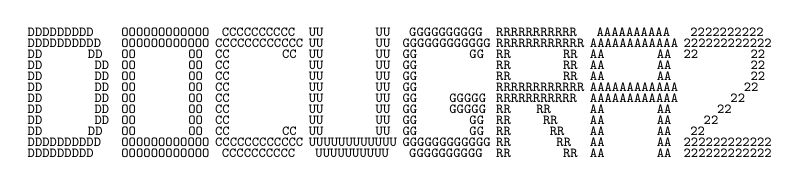
\begin{tikzpicture}[x=.085cm,y=.14cm]
\node[anchor=base west,inner sep=0pt,font=\tiny\ttfamily] at (0,0) {DDDDDDDDD};
\node[anchor=base west,inner sep=0pt,font=\tiny\ttfamily] at (0,-1) {DDDDDDDDDD};
\node[anchor=base west,inner sep=0pt,font=\tiny\ttfamily] at (0,-2) {DD};
\node[anchor=base west,inner sep=0pt,font=\tiny\ttfamily] at (9,-2) {DD};
\node[anchor=base west,inner sep=0pt,font=\tiny\ttfamily] at (0,-3) {DD};
\node[anchor=base west,inner sep=0pt,font=\tiny\ttfamily] at (10,-3) {DD};
\node[anchor=base west,inner sep=0pt,font=\tiny\ttfamily] at (0,-4) {DD};
\node[anchor=base west,inner sep=0pt,font=\tiny\ttfamily] at (10,-4) {DD};
\node[anchor=base west,inner sep=0pt,font=\tiny\ttfamily] at (0,-5) {DD};
\node[anchor=base west,inner sep=0pt,font=\tiny\ttfamily] at (10,-5) {DD};
\node[anchor=base west,inner sep=0pt,font=\tiny\ttfamily] at (0,-6) {DD};
\node[anchor=base west,inner sep=0pt,font=\tiny\ttfamily] at (10,-6) {DD};
\node[anchor=base west,inner sep=0pt,font=\tiny\ttfamily] at (0,-7) {DD};
\node[anchor=base west,inner sep=0pt,font=\tiny\ttfamily] at (10,-7) {DD};
\node[anchor=base west,inner sep=0pt,font=\tiny\ttfamily] at (0,-8) {DD};
\node[anchor=base west,inner sep=0pt,font=\tiny\ttfamily] at (10,-8) {DD};
\node[anchor=base west,inner sep=0pt,font=\tiny\ttfamily] at (0,-9) {DD};
\node[anchor=base west,inner sep=0pt,font=\tiny\ttfamily] at (9,-9) {DD};
\node[anchor=base west,inner sep=0pt,font=\tiny\ttfamily] at (0,-10) {DDDDDDDDDD};
\node[anchor=base west,inner sep=0pt,font=\tiny\ttfamily] at (0,-11) {DDDDDDDDD};
\node[anchor=base west,inner sep=0pt,font=\tiny\ttfamily] at (14,0) {OOOOOOOOOOOO};
\node[anchor=base west,inner sep=0pt,font=\tiny\ttfamily] at (14,-1) {OOOOOOOOOOOO};
\node[anchor=base west,inner sep=0pt,font=\tiny\ttfamily] at (14,-2) {OO};
\node[anchor=base west,inner sep=0pt,font=\tiny\ttfamily] at (24,-2) {OO};
\node[anchor=base west,inner sep=0pt,font=\tiny\ttfamily] at (14,-3) {OO};
\node[anchor=base west,inner sep=0pt,font=\tiny\ttfamily] at (24,-3) {OO};
\node[anchor=base west,inner sep=0pt,font=\tiny\ttfamily] at (14,-4) {OO};
\node[anchor=base west,inner sep=0pt,font=\tiny\ttfamily] at (24,-4) {OO};
\node[anchor=base west,inner sep=0pt,font=\tiny\ttfamily] at (14,-5) {OO};
\node[anchor=base west,inner sep=0pt,font=\tiny\ttfamily] at (24,-5) {OO};
\node[anchor=base west,inner sep=0pt,font=\tiny\ttfamily] at (14,-6) {OO};
\node[anchor=base west,inner sep=0pt,font=\tiny\ttfamily] at (24,-6) {OO};
\node[anchor=base west,inner sep=0pt,font=\tiny\ttfamily] at (14,-7) {OO};
\node[anchor=base west,inner sep=0pt,font=\tiny\ttfamily] at (24,-7) {OO};
\node[anchor=base west,inner sep=0pt,font=\tiny\ttfamily] at (14,-8) {OO};
\node[anchor=base west,inner sep=0pt,font=\tiny\ttfamily] at (24,-8) {OO};
\node[anchor=base west,inner sep=0pt,font=\tiny\ttfamily] at (14,-9) {OO};
\node[anchor=base west,inner sep=0pt,font=\tiny\ttfamily] at (24,-9) {OO};
\node[anchor=base west,inner sep=0pt,font=\tiny\ttfamily] at (14,-10) {OOOOOOOOOOOO};
\node[anchor=base west,inner sep=0pt,font=\tiny\ttfamily] at (14,-11) {OOOOOOOOOOOO};
\node[anchor=base west,inner sep=0pt,font=\tiny\ttfamily] at (29,0) {CCCCCCCCCC};
\node[anchor=base west,inner sep=0pt,font=\tiny\ttfamily] at (28,-1) {CCCCCCCCCCCC};
\node[anchor=base west,inner sep=0pt,font=\tiny\ttfamily] at (28,-2) {CC};
\node[anchor=base west,inner sep=0pt,font=\tiny\ttfamily] at (38,-2) {CC};
\node[anchor=base west,inner sep=0pt,font=\tiny\ttfamily] at (28,-3) {CC};
\node[anchor=base west,inner sep=0pt,font=\tiny\ttfamily] at (28,-4) {CC};
\node[anchor=base west,inner sep=0pt,font=\tiny\ttfamily] at (28,-5) {CC};
\node[anchor=base west,inner sep=0pt,font=\tiny\ttfamily] at (28,-6) {CC};
\node[anchor=base west,inner sep=0pt,font=\tiny\ttfamily] at (28,-7) {CC};
\node[anchor=base west,inner sep=0pt,font=\tiny\ttfamily] at (28,-8) {CC};
\node[anchor=base west,inner sep=0pt,font=\tiny\ttfamily] at (28,-9) {CC};
\node[anchor=base west,inner sep=0pt,font=\tiny\ttfamily] at (38,-9) {CC};
\node[anchor=base west,inner sep=0pt,font=\tiny\ttfamily] at (28,-10) {CCCCCCCCCCCC};
\node[anchor=base west,inner sep=0pt,font=\tiny\ttfamily] at (29,-11) {CCCCCCCCCC};
\node[anchor=base west,inner sep=0pt,font=\tiny\ttfamily] at (42,0) {UU};
\node[anchor=base west,inner sep=0pt,font=\tiny\ttfamily] at (52,0) {UU};
\node[anchor=base west,inner sep=0pt,font=\tiny\ttfamily] at (42,-1) {UU};
\node[anchor=base west,inner sep=0pt,font=\tiny\ttfamily] at (52,-1) {UU};
\node[anchor=base west,inner sep=0pt,font=\tiny\ttfamily] at (42,-2) {UU};
\node[anchor=base west,inner sep=0pt,font=\tiny\ttfamily] at (52,-2) {UU};
\node[anchor=base west,inner sep=0pt,font=\tiny\ttfamily] at (42,-3) {UU};
\node[anchor=base west,inner sep=0pt,font=\tiny\ttfamily] at (52,-3) {UU};
\node[anchor=base west,inner sep=0pt,font=\tiny\ttfamily] at (42,-4) {UU};
\node[anchor=base west,inner sep=0pt,font=\tiny\ttfamily] at (52,-4) {UU};
\node[anchor=base west,inner sep=0pt,font=\tiny\ttfamily] at (42,-5) {UU};
\node[anchor=base west,inner sep=0pt,font=\tiny\ttfamily] at (52,-5) {UU};
\node[anchor=base west,inner sep=0pt,font=\tiny\ttfamily] at (42,-6) {UU};
\node[anchor=base west,inner sep=0pt,font=\tiny\ttfamily] at (52,-6) {UU};
\node[anchor=base west,inner sep=0pt,font=\tiny\ttfamily] at (42,-7) {UU};
\node[anchor=base west,inner sep=0pt,font=\tiny\ttfamily] at (52,-7) {UU};
\node[anchor=base west,inner sep=0pt,font=\tiny\ttfamily] at (42,-8) {UU};
\node[anchor=base west,inner sep=0pt,font=\tiny\ttfamily] at (52,-8) {UU};
\node[anchor=base west,inner sep=0pt,font=\tiny\ttfamily] at (42,-9) {UU};
\node[anchor=base west,inner sep=0pt,font=\tiny\ttfamily] at (52,-9) {UU};
\node[anchor=base west,inner sep=0pt,font=\tiny\ttfamily] at (42,-10) {UUUUUUUUUUUU};
\node[anchor=base west,inner sep=0pt,font=\tiny\ttfamily] at (43,-11) {UUUUUUUUUU};
\node[anchor=base west,inner sep=0pt,font=\tiny\ttfamily] at (57,0) {GGGGGGGGGG};
\node[anchor=base west,inner sep=0pt,font=\tiny\ttfamily] at (56,-1) {GGGGGGGGGGGG};
\node[anchor=base west,inner sep=0pt,font=\tiny\ttfamily] at (56,-2) {GG};
\node[anchor=base west,inner sep=0pt,font=\tiny\ttfamily] at (66,-2) {GG};
\node[anchor=base west,inner sep=0pt,font=\tiny\ttfamily] at (56,-3) {GG};
\node[anchor=base west,inner sep=0pt,font=\tiny\ttfamily] at (56,-4) {GG};
\node[anchor=base west,inner sep=0pt,font=\tiny\ttfamily] at (56,-5) {GG};
\node[anchor=base west,inner sep=0pt,font=\tiny\ttfamily] at (56,-6) {GG};
\node[anchor=base west,inner sep=0pt,font=\tiny\ttfamily] at (63,-6) {GGGGG};
\node[anchor=base west,inner sep=0pt,font=\tiny\ttfamily] at (56,-7) {GG};
\node[anchor=base west,inner sep=0pt,font=\tiny\ttfamily] at (63,-7) {GGGGG};
\node[anchor=base west,inner sep=0pt,font=\tiny\ttfamily] at (56,-8) {GG};
\node[anchor=base west,inner sep=0pt,font=\tiny\ttfamily] at (66,-8) {GG};
\node[anchor=base west,inner sep=0pt,font=\tiny\ttfamily] at (56,-9) {GG};
\node[anchor=base west,inner sep=0pt,font=\tiny\ttfamily] at (66,-9) {GG};
\node[anchor=base west,inner sep=0pt,font=\tiny\ttfamily] at (56,-10) {GGGGGGGGGGGG};
\node[anchor=base west,inner sep=0pt,font=\tiny\ttfamily] at (57,-11) {GGGGGGGGGG};
\node[anchor=base west,inner sep=0pt,font=\tiny\ttfamily] at (70,0) {RRRRRRRRRRR};
\node[anchor=base west,inner sep=0pt,font=\tiny\ttfamily] at (70,-1) {RRRRRRRRRRRR};
\node[anchor=base west,inner sep=0pt,font=\tiny\ttfamily] at (70,-2) {RR};
\node[anchor=base west,inner sep=0pt,font=\tiny\ttfamily] at (80,-2) {RR};
\node[anchor=base west,inner sep=0pt,font=\tiny\ttfamily] at (70,-3) {RR};
\node[anchor=base west,inner sep=0pt,font=\tiny\ttfamily] at (80,-3) {RR};
\node[anchor=base west,inner sep=0pt,font=\tiny\ttfamily] at (70,-4) {RR};
\node[anchor=base west,inner sep=0pt,font=\tiny\ttfamily] at (80,-4) {RR};
\node[anchor=base west,inner sep=0pt,font=\tiny\ttfamily] at (70,-5) {RRRRRRRRRRRR};
\node[anchor=base west,inner sep=0pt,font=\tiny\ttfamily] at (70,-6) {RRRRRRRRRRR};
\node[anchor=base west,inner sep=0pt,font=\tiny\ttfamily] at (70,-7) {RR};
\node[anchor=base west,inner sep=0pt,font=\tiny\ttfamily] at (76,-7) {RR};
\node[anchor=base west,inner sep=0pt,font=\tiny\ttfamily] at (70,-8) {RR};
\node[anchor=base west,inner sep=0pt,font=\tiny\ttfamily] at (77,-8) {RR};
\node[anchor=base west,inner sep=0pt,font=\tiny\ttfamily] at (70,-9) {RR};
\node[anchor=base west,inner sep=0pt,font=\tiny\ttfamily] at (78,-9) {RR};
\node[anchor=base west,inner sep=0pt,font=\tiny\ttfamily] at (70,-10) {RR};
\node[anchor=base west,inner sep=0pt,font=\tiny\ttfamily] at (79,-10) {RR};
\node[anchor=base west,inner sep=0pt,font=\tiny\ttfamily] at (70,-11) {RR};
\node[anchor=base west,inner sep=0pt,font=\tiny\ttfamily] at (80,-11) {RR};
\node[anchor=base west,inner sep=0pt,font=\tiny\ttfamily] at (85,0) {AAAAAAAAAA};
\node[anchor=base west,inner sep=0pt,font=\tiny\ttfamily] at (84,-1) {AAAAAAAAAAAA};
\node[anchor=base west,inner sep=0pt,font=\tiny\ttfamily] at (84,-2) {AA};
\node[anchor=base west,inner sep=0pt,font=\tiny\ttfamily] at (94,-2) {AA};
\node[anchor=base west,inner sep=0pt,font=\tiny\ttfamily] at (84,-3) {AA};
\node[anchor=base west,inner sep=0pt,font=\tiny\ttfamily] at (94,-3) {AA};
\node[anchor=base west,inner sep=0pt,font=\tiny\ttfamily] at (84,-4) {AA};
\node[anchor=base west,inner sep=0pt,font=\tiny\ttfamily] at (94,-4) {AA};
\node[anchor=base west,inner sep=0pt,font=\tiny\ttfamily] at (84,-5) {AAAAAAAAAAAA};
\node[anchor=base west,inner sep=0pt,font=\tiny\ttfamily] at (84,-6) {AAAAAAAAAAAA};
\node[anchor=base west,inner sep=0pt,font=\tiny\ttfamily] at (84,-7) {AA};
\node[anchor=base west,inner sep=0pt,font=\tiny\ttfamily] at (94,-7) {AA};
\node[anchor=base west,inner sep=0pt,font=\tiny\ttfamily] at (84,-8) {AA};
\node[anchor=base west,inner sep=0pt,font=\tiny\ttfamily] at (94,-8) {AA};
\node[anchor=base west,inner sep=0pt,font=\tiny\ttfamily] at (84,-9) {AA};
\node[anchor=base west,inner sep=0pt,font=\tiny\ttfamily] at (94,-9) {AA};
\node[anchor=base west,inner sep=0pt,font=\tiny\ttfamily] at (84,-10) {AA};
\node[anchor=base west,inner sep=0pt,font=\tiny\ttfamily] at (94,-10) {AA};
\node[anchor=base west,inner sep=0pt,font=\tiny\ttfamily] at (84,-11) {AA};
\node[anchor=base west,inner sep=0pt,font=\tiny\ttfamily] at (94,-11) {AA};
\node[anchor=base west,inner sep=0pt,font=\tiny\ttfamily] at (99,0) {2222222222};
\node[anchor=base west,inner sep=0pt,font=\tiny\ttfamily] at (98,-1) {222222222222};
\node[anchor=base west,inner sep=0pt,font=\tiny\ttfamily] at (98,-2) {22};
\node[anchor=base west,inner sep=0pt,font=\tiny\ttfamily] at (108,-2) {22};
\node[anchor=base west,inner sep=0pt,font=\tiny\ttfamily] at (108,-3) {22};
\node[anchor=base west,inner sep=0pt,font=\tiny\ttfamily] at (108,-4) {22};
\node[anchor=base west,inner sep=0pt,font=\tiny\ttfamily] at (107,-5) {22};
\node[anchor=base west,inner sep=0pt,font=\tiny\ttfamily] at (105,-6) {22};
\node[anchor=base west,inner sep=0pt,font=\tiny\ttfamily] at (103,-7) {22};
\node[anchor=base west,inner sep=0pt,font=\tiny\ttfamily] at (101,-8) {22};
\node[anchor=base west,inner sep=0pt,font=\tiny\ttfamily] at (99,-9) {22};
\node[anchor=base west,inner sep=0pt,font=\tiny\ttfamily] at (98,-10) {222222222222};
\node[anchor=base west,inner sep=0pt,font=\tiny\ttfamily] at (98,-11) {222222222222};
\end{tikzpicture}}

\texttt{****A\quad END\quad JOB\quad 5\quad DOCUGRA2\qquad ROOM\qquad 2.28.52 PM 24 AUG 82\quad R6.PR1\quad SYS JES2\quad JOB\quad 5\quad END\quad A****}

\texttt{****A\quad END\quad JOB\quad 5\quad DOCUGRA2\qquad ROOM\qquad 2.28.52 PM 24 AUG 82\quad R6.PR1\quad SYS JES2\quad JOB\quad 5\quad END\quad A****}

\texttt{****A\quad END\quad JOB\quad 5\quad DOCUGRA2\qquad ROOM\qquad 2.28.52 PM 24 AUG 82\quad R6.PR1\quad SYS JES2\quad JOB\quad 5\quad END\quad A****}

\texttt{****A\quad END\quad JOB\quad 5\quad DOCUGRA2\qquad ROOM\qquad 2.28.52 PM 24 AUG 82\quad R6.PR1\quad SYS JES2\quad JOB\quad 5\quad END\quad A****}

\texttt{****A\quad END\quad JOB\quad 5\quad DOCUGRA2\qquad ROOM\qquad 2.28.52 PM 24 AUG 82\quad R6.PR1\quad SYS JES2\quad JOB\quad 5\quad END\quad A****}

\texttt{****A\quad END\quad JOB\quad 5\quad DOCUGRA2\qquad ROOM\qquad 2.28.52 PM 24 AUG 82\quad R6.PR1\quad SYS JES2\quad JOB\quad 5\quad END\quad A****}

\diagram{\begin{tikzcd}[column sep=large,row sep=large]
x\arrow[drr]\arrow[ddr] &&x\arrow[d,hook,shift left=1]\\
&&x'\arrow[u,hook,shift left=1]\arrow[dl,shift right=1]\\
&x''\arrow[ur,hook,very thick,shift right=1]&
\end{tikzcd}}

\diagram{\begin{tikzcd}
x\arrow[dr]&x\arrow[d,"\sim"]\\
\deleted{x}\arrow[r,phantom,"\deleted{\unsure{\longrightarrow}}" description]&\bar x
\end{tikzcd}}

\diagram{\begin{tikzcd}
\widetilde C\arrow[r,"\unsure{\Phi|\varphi}"]&W^{-1}C
\end{tikzcd}}

\mspage{12}

\scanpage{14}
\mspage{7})

qu'on compose encore comme précédemment. On a bien \deleted{\unsure{deux|un}} \unsure{foncteurs|foncteur}
\diagram{\begin{tikzcd}
\deleted{\unsure{C\longrightarrow}}&\widetilde C\arrow[r]&W^{-1}C
\end{tikzcd}}

\deleted{Le premier de ces deux foncteurs transforme bien les éléments de $W$ en flèches inversibles. \deleted{On a} Pour
\diagram{\begin{tikzcd}
x\arrow[r,"f","\sim"']&y
\end{tikzcd}}
\unsure{$f\in W$}, on considère
\[\text{soit }F=[f]\]
\diagram{\begin{tikzcd}
y\arrow[dr,"1_y"']&x\arrow[d,"f","\sim"']\\
&y
\end{tikzcd}}
\[\text{soit }G=[1_y,f].\]
\unsure{Et on trouve les composés} \unsure{et on a donc}
\[\uline{GF}=\unsure{[\,]^{x}}\]
}
\unsure{définissons le} $=$
\diagram{\begin{tikzcd}C\arrow[r]&\widetilde C\end{tikzcd}}
qui va être un peu plus délicat. Soit $f:x\longrightarrow y$. On choisit une factorisation
\diagram{\begin{tikzcd}[column sep=large,row sep=large]
x\arrow[dr,hook,"f_0"']&y\arrow[dr,bend left=30,dotted,"i"]\arrow[dr,dashed,"\beta","\sim"']&\\
&\bar y\arrow[u,"\unsure{\alpha}","\sim"']\arrow[r,dotted,"\unsure{g}","\sim"']&\bar y'
\end{tikzcd}}
\inserted{\unsure{donc $\bar y$ cof}}
et, avec le \unsure{w.k lifting lemma} (ici $y$ étant cofibrant) on peut compléter par des pointillés, où $\beta$ a une section $i$.

On considère alors $[g f_0,i]$, il faut montrer que ça ne dépend pas des choix faits. Pour un choix $[f',i']$
\diagram{\begin{tikzcd}
x\arrow[r,dashed,"f"]\arrow[dr,"f'"']&y\arrow[d,"i'","\sim"',shift right=1]\\
&y'\arrow[u,dashed,"\alpha","\sim"',shift right=1]
\end{tikzcd}}
tel qu'il existe \deleted{\unsure{un|une}} une rétraction $\alpha$ de $\widetilde y$ sur $y$, telle que
\[\alpha f'=f.\]

\margin{On s'est ramené aux factorisations $f=\unsure{\alpha}f_0$, $\unsure{f_0}\in\unsure{\operatorname{cof}}$ et $\unsure{\alpha}\in W$, telles que $\unsure{\alpha}$ ait une section.}

Considérons deux tels choix, il faut voir qu'ils sont dans une $=$ composante connexe de $\underline{\operatorname{Ch}}_0(x,y)$. Mais pour deux factorisations d'une flèche $f:x\longrightarrow y$ en $\alpha f_0$ et $\alpha'f'_0$, $f_0,f'_0\in\operatorname{Cof}$, $\alpha,\alpha'\in W$, \deleted{\unsure{$x\longrightarrow y$}} on peut les coiffer par une troisième \deleted{\unsure{$f''$}} $\alpha'',f''_0$ qui \deleted{\unsure{\diagram{\begin{tikzcd}x\arrow[r]&y''\end{tikzcd}}}} \deleted{\unsure{permet de}} \inserted{\unsure{reçoit|réduit}} les deux \unsure{comme on voit dans les diagrammes}

\margin{Ce foncteur est bijectif sur les objets, surjectif sur les flèches, \unsure{comme préc.}. On vérifie aisément [il suffit pour cela \unsure{dans un produit} de voir que pour tt $f\in W$, $f:x\longrightarrow y$, $[f]^{-1}$ provient de $\widetilde C$, on prend
\diagram{\begin{tikzcd}
x\arrow[r,"\unsure{f}"]\arrow[dr,"\sim"']&y\arrow[d,shift left=1,"\alpha"]\\
&\unsure{\bar y}\arrow[u,very thick,shift left=1,"\unsure{i}","\sim"']
\end{tikzcd}}
\unsure{(les deux isos)}]
\diagram{\begin{tikzcd}
y\arrow[dr,"\unsure{1_y}"']&\unsure{x}\arrow[d,"\unsure{f}","\sim"',shift right=1]\\
&y\arrow[u,"\unsure{\alpha}"',shift right=1]
\end{tikzcd}}
}

\figure{\begin{tikzpicture}[x=.4cm,y=.4cm]
\draw (0,.2) .. controls (-1.4,.4) and (-.8,3.2) .. (1.8,5.5) .. controls (3.8,7.3) and (5.4,7.8) .. (5.1,5.4) .. controls (4.8,2.1) and (1.8,-.5) .. (0,.2);
\end{tikzpicture}}
\mspage{13}

\scanpage{15}
\texttt{//*\quad GRAPHI2\quad 0421\quad -\quad CRAYI}

\figure{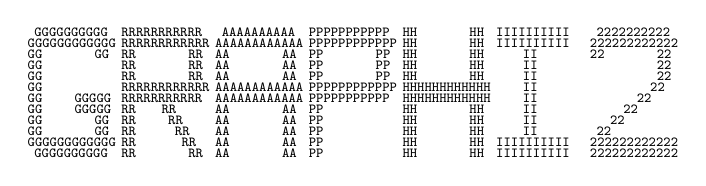
\begin{tikzpicture}[x=.085cm,y=.14cm]
\node[anchor=base west,inner sep=0pt,font=\tiny\ttfamily] at (1,0) {GGGGGGGGGG};
\node[anchor=base west,inner sep=0pt,font=\tiny\ttfamily] at (0,-1) {GGGGGGGGGGGG};
\node[anchor=base west,inner sep=0pt,font=\tiny\ttfamily] at (0,-2) {GG};
\node[anchor=base west,inner sep=0pt,font=\tiny\ttfamily] at (10,-2) {GG};
\node[anchor=base west,inner sep=0pt,font=\tiny\ttfamily] at (0,-3) {GG};
\node[anchor=base west,inner sep=0pt,font=\tiny\ttfamily] at (0,-4) {GG};
\node[anchor=base west,inner sep=0pt,font=\tiny\ttfamily] at (0,-5) {GG};
\node[anchor=base west,inner sep=0pt,font=\tiny\ttfamily] at (0,-6) {GG};
\node[anchor=base west,inner sep=0pt,font=\tiny\ttfamily] at (7,-6) {GGGGG};
\node[anchor=base west,inner sep=0pt,font=\tiny\ttfamily] at (0,-7) {GG};
\node[anchor=base west,inner sep=0pt,font=\tiny\ttfamily] at (7,-7) {GGGGG};
\node[anchor=base west,inner sep=0pt,font=\tiny\ttfamily] at (0,-8) {GG};
\node[anchor=base west,inner sep=0pt,font=\tiny\ttfamily] at (10,-8) {GG};
\node[anchor=base west,inner sep=0pt,font=\tiny\ttfamily] at (0,-9) {GG};
\node[anchor=base west,inner sep=0pt,font=\tiny\ttfamily] at (10,-9) {GG};
\node[anchor=base west,inner sep=0pt,font=\tiny\ttfamily] at (0,-10) {GGGGGGGGGGGG};
\node[anchor=base west,inner sep=0pt,font=\tiny\ttfamily] at (1,-11) {GGGGGGGGGG};
\node[anchor=base west,inner sep=0pt,font=\tiny\ttfamily] at (14,0) {RRRRRRRRRRR};
\node[anchor=base west,inner sep=0pt,font=\tiny\ttfamily] at (14,-1) {RRRRRRRRRRRR};
\node[anchor=base west,inner sep=0pt,font=\tiny\ttfamily] at (14,-2) {RR};
\node[anchor=base west,inner sep=0pt,font=\tiny\ttfamily] at (24,-2) {RR};
\node[anchor=base west,inner sep=0pt,font=\tiny\ttfamily] at (14,-3) {RR};
\node[anchor=base west,inner sep=0pt,font=\tiny\ttfamily] at (24,-3) {RR};
\node[anchor=base west,inner sep=0pt,font=\tiny\ttfamily] at (14,-4) {RR};
\node[anchor=base west,inner sep=0pt,font=\tiny\ttfamily] at (24,-4) {RR};
\node[anchor=base west,inner sep=0pt,font=\tiny\ttfamily] at (14,-5) {RRRRRRRRRRRR};
\node[anchor=base west,inner sep=0pt,font=\tiny\ttfamily] at (14,-6) {RRRRRRRRRRR};
\node[anchor=base west,inner sep=0pt,font=\tiny\ttfamily] at (14,-7) {RR};
\node[anchor=base west,inner sep=0pt,font=\tiny\ttfamily] at (20,-7) {RR};
\node[anchor=base west,inner sep=0pt,font=\tiny\ttfamily] at (14,-8) {RR};
\node[anchor=base west,inner sep=0pt,font=\tiny\ttfamily] at (21,-8) {RR};
\node[anchor=base west,inner sep=0pt,font=\tiny\ttfamily] at (14,-9) {RR};
\node[anchor=base west,inner sep=0pt,font=\tiny\ttfamily] at (22,-9) {RR};
\node[anchor=base west,inner sep=0pt,font=\tiny\ttfamily] at (14,-10) {RR};
\node[anchor=base west,inner sep=0pt,font=\tiny\ttfamily] at (23,-10) {RR};
\node[anchor=base west,inner sep=0pt,font=\tiny\ttfamily] at (14,-11) {RR};
\node[anchor=base west,inner sep=0pt,font=\tiny\ttfamily] at (24,-11) {RR};
\node[anchor=base west,inner sep=0pt,font=\tiny\ttfamily] at (29,0) {AAAAAAAAAA};
\node[anchor=base west,inner sep=0pt,font=\tiny\ttfamily] at (28,-1) {AAAAAAAAAAAA};
\node[anchor=base west,inner sep=0pt,font=\tiny\ttfamily] at (28,-2) {AA};
\node[anchor=base west,inner sep=0pt,font=\tiny\ttfamily] at (38,-2) {AA};
\node[anchor=base west,inner sep=0pt,font=\tiny\ttfamily] at (28,-3) {AA};
\node[anchor=base west,inner sep=0pt,font=\tiny\ttfamily] at (38,-3) {AA};
\node[anchor=base west,inner sep=0pt,font=\tiny\ttfamily] at (28,-4) {AA};
\node[anchor=base west,inner sep=0pt,font=\tiny\ttfamily] at (38,-4) {AA};
\node[anchor=base west,inner sep=0pt,font=\tiny\ttfamily] at (28,-5) {AAAAAAAAAAAA};
\node[anchor=base west,inner sep=0pt,font=\tiny\ttfamily] at (28,-6) {AAAAAAAAAAAA};
\node[anchor=base west,inner sep=0pt,font=\tiny\ttfamily] at (28,-7) {AA};
\node[anchor=base west,inner sep=0pt,font=\tiny\ttfamily] at (38,-7) {AA};
\node[anchor=base west,inner sep=0pt,font=\tiny\ttfamily] at (28,-8) {AA};
\node[anchor=base west,inner sep=0pt,font=\tiny\ttfamily] at (38,-8) {AA};
\node[anchor=base west,inner sep=0pt,font=\tiny\ttfamily] at (28,-9) {AA};
\node[anchor=base west,inner sep=0pt,font=\tiny\ttfamily] at (38,-9) {AA};
\node[anchor=base west,inner sep=0pt,font=\tiny\ttfamily] at (28,-10) {AA};
\node[anchor=base west,inner sep=0pt,font=\tiny\ttfamily] at (38,-10) {AA};
\node[anchor=base west,inner sep=0pt,font=\tiny\ttfamily] at (28,-11) {AA};
\node[anchor=base west,inner sep=0pt,font=\tiny\ttfamily] at (38,-11) {AA};
\node[anchor=base west,inner sep=0pt,font=\tiny\ttfamily] at (42,0) {PPPPPPPPPPP};
\node[anchor=base west,inner sep=0pt,font=\tiny\ttfamily] at (42,-1) {PPPPPPPPPPPP};
\node[anchor=base west,inner sep=0pt,font=\tiny\ttfamily] at (42,-2) {PP};
\node[anchor=base west,inner sep=0pt,font=\tiny\ttfamily] at (52,-2) {PP};
\node[anchor=base west,inner sep=0pt,font=\tiny\ttfamily] at (42,-3) {PP};
\node[anchor=base west,inner sep=0pt,font=\tiny\ttfamily] at (52,-3) {PP};
\node[anchor=base west,inner sep=0pt,font=\tiny\ttfamily] at (42,-4) {PP};
\node[anchor=base west,inner sep=0pt,font=\tiny\ttfamily] at (52,-4) {PP};
\node[anchor=base west,inner sep=0pt,font=\tiny\ttfamily] at (42,-5) {PPPPPPPPPPPP};
\node[anchor=base west,inner sep=0pt,font=\tiny\ttfamily] at (42,-6) {PPPPPPPPPPP};
\node[anchor=base west,inner sep=0pt,font=\tiny\ttfamily] at (42,-7) {PP};
\node[anchor=base west,inner sep=0pt,font=\tiny\ttfamily] at (42,-8) {PP};
\node[anchor=base west,inner sep=0pt,font=\tiny\ttfamily] at (42,-9) {PP};
\node[anchor=base west,inner sep=0pt,font=\tiny\ttfamily] at (42,-10) {PP};
\node[anchor=base west,inner sep=0pt,font=\tiny\ttfamily] at (42,-11) {PP};
\node[anchor=base west,inner sep=0pt,font=\tiny\ttfamily] at (56,0) {HH};
\node[anchor=base west,inner sep=0pt,font=\tiny\ttfamily] at (66,0) {HH};
\node[anchor=base west,inner sep=0pt,font=\tiny\ttfamily] at (56,-1) {HH};
\node[anchor=base west,inner sep=0pt,font=\tiny\ttfamily] at (66,-1) {HH};
\node[anchor=base west,inner sep=0pt,font=\tiny\ttfamily] at (56,-2) {HH};
\node[anchor=base west,inner sep=0pt,font=\tiny\ttfamily] at (66,-2) {HH};
\node[anchor=base west,inner sep=0pt,font=\tiny\ttfamily] at (56,-3) {HH};
\node[anchor=base west,inner sep=0pt,font=\tiny\ttfamily] at (66,-3) {HH};
\node[anchor=base west,inner sep=0pt,font=\tiny\ttfamily] at (56,-4) {HH};
\node[anchor=base west,inner sep=0pt,font=\tiny\ttfamily] at (66,-4) {HH};
\node[anchor=base west,inner sep=0pt,font=\tiny\ttfamily] at (56,-5) {HHHHHHHHHHHH};
\node[anchor=base west,inner sep=0pt,font=\tiny\ttfamily] at (56,-6) {HHHHHHHHHHHH};
\node[anchor=base west,inner sep=0pt,font=\tiny\ttfamily] at (56,-7) {HH};
\node[anchor=base west,inner sep=0pt,font=\tiny\ttfamily] at (66,-7) {HH};
\node[anchor=base west,inner sep=0pt,font=\tiny\ttfamily] at (56,-8) {HH};
\node[anchor=base west,inner sep=0pt,font=\tiny\ttfamily] at (66,-8) {HH};
\node[anchor=base west,inner sep=0pt,font=\tiny\ttfamily] at (56,-9) {HH};
\node[anchor=base west,inner sep=0pt,font=\tiny\ttfamily] at (66,-9) {HH};
\node[anchor=base west,inner sep=0pt,font=\tiny\ttfamily] at (56,-10) {HH};
\node[anchor=base west,inner sep=0pt,font=\tiny\ttfamily] at (66,-10) {HH};
\node[anchor=base west,inner sep=0pt,font=\tiny\ttfamily] at (56,-11) {HH};
\node[anchor=base west,inner sep=0pt,font=\tiny\ttfamily] at (66,-11) {HH};
\node[anchor=base west,inner sep=0pt,font=\tiny\ttfamily] at (70,0) {IIIIIIIIII};
\node[anchor=base west,inner sep=0pt,font=\tiny\ttfamily] at (70,-1) {IIIIIIIIII};
\node[anchor=base west,inner sep=0pt,font=\tiny\ttfamily] at (74,-2) {II};
\node[anchor=base west,inner sep=0pt,font=\tiny\ttfamily] at (74,-3) {II};
\node[anchor=base west,inner sep=0pt,font=\tiny\ttfamily] at (74,-4) {II};
\node[anchor=base west,inner sep=0pt,font=\tiny\ttfamily] at (74,-5) {II};
\node[anchor=base west,inner sep=0pt,font=\tiny\ttfamily] at (74,-6) {II};
\node[anchor=base west,inner sep=0pt,font=\tiny\ttfamily] at (74,-7) {II};
\node[anchor=base west,inner sep=0pt,font=\tiny\ttfamily] at (74,-8) {II};
\node[anchor=base west,inner sep=0pt,font=\tiny\ttfamily] at (74,-9) {II};
\node[anchor=base west,inner sep=0pt,font=\tiny\ttfamily] at (70,-10) {IIIIIIIIII};
\node[anchor=base west,inner sep=0pt,font=\tiny\ttfamily] at (70,-11) {IIIIIIIIII};
\node[anchor=base west,inner sep=0pt,font=\tiny\ttfamily] at (85,0) {2222222222};
\node[anchor=base west,inner sep=0pt,font=\tiny\ttfamily] at (84,-1) {222222222222};
\node[anchor=base west,inner sep=0pt,font=\tiny\ttfamily] at (84,-2) {22};
\node[anchor=base west,inner sep=0pt,font=\tiny\ttfamily] at (94,-2) {22};
\node[anchor=base west,inner sep=0pt,font=\tiny\ttfamily] at (94,-3) {22};
\node[anchor=base west,inner sep=0pt,font=\tiny\ttfamily] at (94,-4) {22};
\node[anchor=base west,inner sep=0pt,font=\tiny\ttfamily] at (93,-5) {22};
\node[anchor=base west,inner sep=0pt,font=\tiny\ttfamily] at (91,-6) {22};
\node[anchor=base west,inner sep=0pt,font=\tiny\ttfamily] at (89,-7) {22};
\node[anchor=base west,inner sep=0pt,font=\tiny\ttfamily] at (87,-8) {22};
\node[anchor=base west,inner sep=0pt,font=\tiny\ttfamily] at (85,-9) {22};
\node[anchor=base west,inner sep=0pt,font=\tiny\ttfamily] at (84,-10) {222222222222};
\node[anchor=base west,inner sep=0pt,font=\tiny\ttfamily] at (84,-11) {222222222222};
\end{tikzpicture}}

\texttt{****A\quad END\quad JOB\quad 421\quad GRAPHI2\quad -\quad CRAY OUTPUT\quad -\qquad ROOM\qquad 3.04.20 PM 25 AUG 82\quad R6.PR1\quad SYS JES2\quad JOB\quad 421\quad END\quad A****}

\texttt{****A\quad END\quad JOB\quad 421\quad GRAPHI2\quad -\quad CRAY OUTPUT\quad -\qquad ROOM\qquad 3.04.20 PM 25 AUG 82\quad R6.PR1\quad SYS JES2\quad JOB\quad 421\quad END\quad A****}

\texttt{****A\quad END\quad JOB\quad 421\quad GRAPHI2\quad -\quad CRAY OUTPUT\quad -\qquad ROOM\qquad 3.04.20 PM 25 AUG 82\quad R6.PR1\quad SYS JES2\quad JOB\quad 421\quad END\quad A****}

\texttt{****A\quad END\quad JOB\quad 421\quad GRAPHI2\quad -\quad CRAY OUTPUT\quad -\qquad ROOM\qquad 3.04.20 PM 25 AUG 82\quad R6.PR1\quad SYS JES2\quad JOB\quad 421\quad END\quad A****}

\texttt{****A\quad END\quad JOB\quad 421\quad GRAPHI2\quad -\quad CRAY OUTPUT\quad -\qquad ROOM\qquad 3.04.20 PM 25 AUG 82\quad R6.PR1\quad SYS JES2\quad JOB\quad 421\quad END\quad A****}

\texttt{****A\quad END\quad JOB\quad 421\quad GRAPHI2\quad -\quad CRAY OUTPUT\quad -\qquad ROOM\qquad 3.04.20 PM 25 AUG 82\quad R6.PR1\quad SYS JES2\quad JOB\quad 421\quad END\quad A****}

\diagram{\begin{tikzcd}[column sep=large,row sep=large]
x\arrow[drr,hook]&&y&\\
&&y'\arrow[u]&y''\arrow[ul]\\
x\amalg x\arrow[rr,hook]\arrow[dr]&&y'\amalg y''\arrow[u]\arrow[d,no head]\arrow[r,leftrightarrow]&\deleted{\unsure{y}}\\
&x\arrow[r,hook]&\unsure{p|\rho}\arrow[r,hook,two heads]&y
\end{tikzcd}}

\diagram{\begin{tikzcd}[column sep=large,row sep=large]
&x\arrow[r,hook]\arrow[d,"i_1"']&y'\arrow[d]\arrow[dl,phantom,"\text{cocart}" description]\\
\deleted{\unsure{y}}\inserted{x}\arrow[r,"i_2"]\arrow[d,hook]&x\amalg x\arrow[r,hook]\arrow[d,hook]&\unsure{y'|x'}\amalg x\arrow[d,hook]\\
y''\arrow[r]&x\amalg y''\arrow[r,hook]&y'\unsure{\amalg}y''
\end{tikzcd}}

\mspage{14}

\scanpage{16}
\mspage{8})

\diagram{\begin{tikzcd}[column sep=large,row sep=large]
x\vee x\arrow[r,hook,"\unsure{\{f_0\vee f'_0\}}"]\arrow[d,"\nabla_x"']&\bar y\amalg\bar y'\arrow[d,dashed]\arrow[drr,"(\alpha,\alpha')"]\arrow[dl,phantom,"\text{cocart}" description]&&\\
x\arrow[r,hook,dashed,"g"]\arrow[rrr,bend right=25,"f"']&\widetilde y\arrow[rr,dashed,"\varphi"']\arrow[r,hook,"\varphi_0"]&\bar y''\arrow[r,dashed,"\alpha''","\sim"']&y
\end{tikzcd}}

on factorise $\varphi$ en $\unsure{\alpha''}\varphi_0$ avec $\varphi_0\in\operatorname{cof}$, $\unsure{\alpha''}\in W$, et on prend
\[f''_0=\varphi_0 g\]

Mais si $\alpha,\alpha'$ ont des sections (il suffirait que $\alpha$ ou $\alpha'$ en ait), \deleted{\unsure{On en a donc}} \inserted{il est trivial que} \deleted{\unsure{la section de}} $\alpha''$ (qui les reçoit) en a aussi une. Donc on est ramené au cas où on a une flèche
\[u:(f_0,\alpha)\longrightarrow(f'_0,\alpha')\]
dans la catégorie des factorisations de $f$ en $\alpha f_0$. Donc \uline{Si} on choisit la section $\unsure{i''|i'}$ pour $\unsure{\alpha''|\alpha'}$ comme l'image par $u$ de la section $\unsure{i'|i''}$ de $\alpha'$ \deleted{\unsure{et}}\unsure{,} on gagne. Donc il reste à prouver que
\diagram{\begin{tikzcd}
x\arrow[rr,"f"]\arrow[dr,"f'_0"']\arrow[drr,"f''_0" description]&&y\\
&\bar y'\arrow[ur,"\alpha'"]\arrow[r,leftrightarrow,"u"']&\bar y''\arrow[u,"\alpha''"']
\end{tikzcd}}
\deleted{le choix de}
pour une factorisation choisie de $f$ en $\alpha f_0$ comme dessus, $[f_0,i]$ ne dépend pas du choix de la section $i$. Comme
\[[f_0,i]=[\operatorname{id}_{\bar y},i]\circ(f,\operatorname{id}_{\bar y}),\]
On est ramené à ceci :

$(\unsure{*})$ Soit
\diagram{\begin{tikzcd}x\arrow[r,"f","\sim"']&y\end{tikzcd}}
dans $W$, tel que $f$ ait une \deleted{\unsure{(deux $i,i'\in W$)}} section $i$, alors \deleted{\unsure{pour deux telles sections $i,i'$}} \inserted{la classe dans} \deleted{les comp. connexes dans} $\pi_0(\underline{\operatorname{Ch}}_0(x,y))$ \deleted{de} des $(1_x,i)$
\diagram{\begin{tikzcd}
\deleted{\unsure{x}}&x\arrow[dr,"1_x"']&y\arrow[d,"i"]\\
&&x
\end{tikzcd}}
ne dépend pas du choix de la section $i$.

\margin{\diagram{\begin{tikzcd}
x\arrow[r,"f^{\unsure{?}}"]\arrow[dr,"f_0"']&y\arrow[d,bend left=15,"i"]\arrow[d,bend left=45,"i'"]\\
&\bar y\arrow[u,"\alpha","\sim"']
\end{tikzcd}}}

Cette condition est (néc. et) \unsure{suffis\textsuperscript{t}} pour que $\widetilde C\mathbin{-}W^{-1}C$ soit fidèle (donc un iso), comme on doit pouvoir vérifier aisément, en construisant bel et bien le foncteur cherché $C\longrightarrow\widetilde C$.

\mspage{15}

\scanpage{17}
\texttt{PAGE 1}\qquad\texttt{ON=CELMPQRSTV}\qquad\texttt{08/25/82-15:01:26}\qquad\texttt{CFT 1.09(06/28/82)}\qquad\texttt{PAGE 1}

\diagram{\begin{array}{rrll}
1&1.& &\texttt{PROGRAM GRAPHI}\\
2&2.& &\texttt{DIMENSION X(10),Y(10)}\\
3&3.& &\texttt{DATA X/0.,0.,4.,9.,1.,2.,0.,0.,1.,0./,}\\
4&&\texttt{S}&\quad\texttt{Y/7.,2.,0.,1.,0.,2.,0.,3.,0.,4./}\\
5&4.& &\texttt{NOL=10}\\
6&5.& &\texttt{XCM=10.}\\
7&6.& &\texttt{YCM=10.}\\
8&7.& &\texttt{N=10}\\
9&8.& &\texttt{WRITE(6,1)}\\
10&9.& &\texttt{CALL TBRAF(NOL,XCM,YCM,0,0,0,0,0,0,0,X,Y,N,0,0.)}\\
11&10.& &\texttt{WRITE(6,2)}\\
12&11.&1&\texttt{FORMAT(' TBRAF VA ETRE APPELE')}\\
13&12.&2&\texttt{FORMAT(' TBRAF A ETE APPELE')}\\
14&13.& &\texttt{STOP}\\
15&14.& &\texttt{END}
\end{array}}

\mspage{16}

\cotefile{107}
\scanpage{2}
\unsure{Formalisme} des

$X\otimes M$, $X^M$, $\underline{\operatorname{Hom}}_A$, $\underline{\operatorname{Hom}}_B$

\unsure{relatifs|relatif} : une rédaction \uline{provisoire}

\texttt{PAGE\qquad 4}

\texttt{ASM 0201 15.27 06/04/82}

\figure{\begin{tikzpicture}[x=.018cm,y=.018cm]
\draw[->] (0,0)--(-105,-155);
\draw (70,-10)--(0,-122);
\draw (130,3)--(70,-100);
\draw (200,-5)..controls(205,-45)and(180,-83)..(170,-110);
\end{tikzpicture}}

\mspage{1}

\scanpage{3}
\diagram{\begin{tikzcd}
& A\times\Delta\arrow[dl,"p_\Delta"']\arrow[dr,"p_A"] &\\
A\arrow[dr,"q_A"'] &&\Delta\arrow[dl,"q_\Delta"]\\
&e&
\end{tikzcd}}
\deleted{
\[
X_*,Y_*\in\mathrm{Ob}\underbrace{(A\times\Delta)^\wedge}_{\simeq\underline{\mathrm{Hom}}(\Delta^o,A^\wedge)\simeq\mathrm{Hom}(A^o,\Delta^\wedge)}
\]
\[
\left\{\begin{aligned}
\mathrm{Hom}_{A\times\Delta}(X_*,Y_*)&=\Gamma_{A\times\Delta}(\underline{\mathrm{Hom}}_{A\times\Delta}(X_*,Y_*))\\
\underline{\mathrm{Hom}}_A(X_*,Y_*)&=p_{\Delta*}\underline{\mathrm{Hom}}_{A\times\Delta}(X_*,Y_*)\\
\underline{\mathrm{Hom}}_\Delta(X_*,Y_*)&=p_{A*}\underline{\mathrm{Hom}}_{A\times\Delta}(X_*,Y_*)
\end{aligned}\right.
\]
\margin{\[
\left\{\begin{aligned}p_{A*}\deleted{\unsure{Y}}X_*&=(\Gamma_A X_n)_n\\p_{\Delta*}X_*&=X_0\end{aligned}\right.
\]
\[(q_\Delta p_A)_*(X_*)=(q_Ap_\Delta)_*X_*=\Gamma_A\unsure{X_0}\]
\figure{\begin{tikzpicture}\draw (0,3)--(1,1.5)--(2.1,.3)--(4.4,.5);\end{tikzpicture}}}
}
\margin{\deleted{\unsure{\mathrm{Hom}}}
\diagram{\begin{tikzcd}
&(A\times\Delta)^\wedge\supset s\underline A=\underline{\mathrm{Hom}}(\Delta^o,A)\arrow[dl,"p_{\Delta*}"']\arrow[dr,"p_{A*}"]&\\
A^\wedge\arrow[dr,"q_{A*}"']&&\Delta^\wedge\arrow[dl,"q_{\Delta*}"]\\
&(\mathrm{Ens})&
\end{tikzcd}}}
\deleted{
\deleted{\unsure{A}} \unsure{What about}
\[
(\underline{\mathrm{Hom}}_A(L,X_n))_n\overset{?}{\in}(A\times\Delta)^\wedge
\]
\[
(\mathrm{Hom}_A(L,X_n))_n\in\Delta^\wedge
\]
for given \(L\in\mathrm{Ob}A^\wedge\) (more generally, \unsure{\(L\in\mathrm{Ob}A^\wedge\)} ?)
the second is the transform of the first by \(p_{A*}\) (\(=\Gamma_A\) applied componentwise).

I contend that if we identify \(L\) with the constant \unsure{complex with value} \(L\), i.e. with \(p_\Delta^*(L)\), we get
\[
(\underline{\mathrm{Hom}}_A(L,X_n))_{n\in\mathbb N}=\underline{\mathrm{Hom}}_{A\times\Delta}(p_\Delta^*(L),X_*)
\]
\margin{hence, by applying \deleted{\unsure{\Gamma_A}} \(p_{A*}\)}
\[
(\mathrm{Hom}_A(L,X_n))_{n\in\mathbb N}=\underline{\mathrm{Hom}}_\Delta(p_\Delta^*(L),X_*)
\]
To get the first one, we apply the definition of \(\underline{\mathrm{Hom}}\), we have to get the \(n^{\mathrm{th}}\) component of the \unsure{second hand side}; \deleted{\unsure{we}} This is easily checked (see below) to be
}
\margin{\(A\)
\diagram{\begin{tikzcd}a_0\arrow[r,leftrightarrow]&a\end{tikzcd}}
\(i_0\in I\qquad I\)}
\margin{\(M(b)\qquad X(a,b)=M(b)\)
\diagram{\begin{tikzcd}
&\{i_0\}\arrow[d,Rightarrow]\\
\underline{\mathrm{Hom}}(\unsure{a|a_1},a_0)\arrow[ur]\arrow[r]&I\\
u\arrow[r,mapsto]&u(i_0)\deleted{\unsure{\varphi}}
\end{tikzcd}}}
\mspage{2}

\scanpage{4}
\mspage{a}
\deleted{\((A\times B)^\wedge\simeq\underline{\mathrm{Hom}}(A^o,B^\wedge)\simeq\underline{\mathrm{Hom}}(B^o,A^\wedge)\).}
\diagram{\begin{tikzcd}&A\times B\arrow[dl,"p_B"']\arrow[dr,"p_A"]&\\A\arrow[dr,"q_A"']&&B\arrow[dl,no head,"q_B"]\\&e&\end{tikzcd}}
\diagram{\begin{tikzcd}[column sep=small]
\underline{\mathrm{Hom}}(A^o,B^\wedge)\arrow[r,phantom,"\simeq"]\arrow[dd,"X'\mapsto\Gamma_B\circ X'"']&(A\times B)^\wedge\arrow[r,phantom,"\simeq"]\arrow[ddl,"(p_B)_*"']\arrow[ddr,"(p_A)_*"]&\underline{\mathrm{Hom}}(B^o,A^\wedge)\arrow[r]\arrow[dd,"X''\mapsto\Gamma_A\circ X''"]&[\underline{\mathrm{Hom}}(B^o,A)]\\
&&&\\
\underline{\mathrm{Hom}}(A^o,(\mathrm{Ens}))\simeq A^\wedge\arrow[dr,"\deleted{\unsure{p_A}}q_{A*}=\Gamma_A=\underline{\mathrm{Hom}}_A(e_{A^\wedge},\cdot)"']&&B^\wedge=\underline{\mathrm{Hom}}(B^o,(\mathrm{Ens}))\arrow[dl,"q_{B*}=\Gamma_B=\underline{\mathrm{Hom}}_B(e_{B^\wedge},\cdot)"]&\\
&(\mathrm{Ens})&&
\end{tikzcd}}
\margin{\[
\begin{aligned}
\underline{\mathrm{Hom}}_B(X,Y)&\overset{\mathrm{def}}=p_{A*}\underline{\mathrm{Hom}}_{A\times B}(X,Y)\\
\underline{\mathrm{Hom}}_A(X,Y)&\overset{\mathrm{def}}=p_{B*}\underline{\mathrm{Hom}}_{A\times B}(X,Y)
\end{aligned}
\]
\deleted{\(\unsure{\mathrm{Hom}(X,Y)=}\)} donc
\[\mathrm{Hom}(X,Y)\simeq\Gamma_{\unsure{A|B}}\underline{\mathrm{Hom}}_A(X,Y)\simeq\Gamma_B\underline{\mathrm{Hom}}_B(X,Y).\]}
\(A\) et \(B\) deux petites catégories.

on travaille dans \((A\times B)^\wedge\simeq\underline{\mathrm{Hom}}(A^o,B^\wedge)\simeq\underline{\mathrm{Hom}}(B^o,A^\wedge)\). On a indiqué sur le diagramme ci-dessus \unsure{qques} propriétés des foncteurs images directes. Pour \(b\in B\), on a un foncteur
\diagram{\begin{tikzcd}
\deleted{\unsure{q_b}}\Gamma_b'':(A\times B)^\wedge\arrow[r,Rightarrow]\arrow[d]&\unsure{A^\wedge}\arrow[d,phantom,"\parallel"]\\
\deleted{\unsure{\simeq}}\underline{\mathrm{Hom}}(B^o,A^\wedge)\arrow[r,no head]&\unsure{A^\wedge}\\
X''\arrow[r,mapsto]&X''(b)\deleted{\unsure{\simeq\mathrm{Hom}}}
\end{tikzcd}}
induit par \((A\times B)^\wedge\simeq\underline{\mathrm{Hom}}(A^o,\unsure{B})\)
\margin{\(\unsure{\downarrow}\)}
Je dis qu'on a
\[
\Gamma_b''(X)\simeq p_{\unsure{B|A}*}\underline{\mathrm{Hom}}(p_{\unsure{A|B}}^*(b),X)\qquad\text{fonctoriel en }b,X
\]
\[
(=\underline{\mathrm{Hom}}_A(p_A^*(b),X));
\]
ce qui signifie aussi qu'on a
\diagram{\begin{tikzcd}[column sep=large]
\mathrm{Hom}_{\unsure{B^\wedge|A^\wedge}}(\unsure{a|b},\Gamma_b''(X))\arrow[r,phantom,"\simeq"]\arrow[d,phantom,"\parallel"]&\mathrm{Hom}_{A^\wedge}(\unsure{a|b},p_{\unsure{B|A}*}\underline{\mathrm{Hom}}(p_A^*(b),X))\arrow[d,phantom,"\wr"]\\
X(a,b)&\mathrm{Hom}_{(A\times B)^\wedge}(p_B^*(a),\underline{\mathrm{Hom}}(p_A^*(b),X))\arrow[d,phantom,"\wr"]\\
&\mathrm{Hom}_{(A\times B)^\wedge}(p_B^*(a)\times p_A^*(b),X)
\end{tikzcd}}
\margin{fonctoriel en \(a,X,b\)\qquad OK}
\deleted{Symétriquement, on a des \(\Gamma_a'\), \(a\in A\)
\diagram{\begin{tikzcd}
\Gamma_a':(A\times B)^\wedge\arrow[r]\arrow[d,phantom,"\wr"]&B^\wedge\\
\underline{\mathrm{Hom}}(A^o,B^\wedge)&\\
X'\arrow[r,mapsto]&X'(a)
\end{tikzcd}}
et on a
\[
\Gamma_a'(X)\simeq p_{A*}(\underline{\mathrm{Hom}}(p_B^*(a),X))
\]}
\mspage{3}

\scanpage{5}
\figure{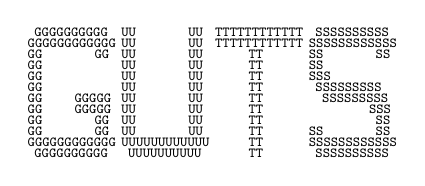
\begin{tikzpicture}[x=.085cm,y=.14cm]
\node[anchor=base west,inner sep=0pt,font=\tiny\ttfamily] at (1,0) {GGGGGGGGGG};
\node[anchor=base west,inner sep=0pt,font=\tiny\ttfamily] at (0,-1) {GGGGGGGGGGGG};
\node[anchor=base west,inner sep=0pt,font=\tiny\ttfamily] at (0,-2) {GG};
\node[anchor=base west,inner sep=0pt,font=\tiny\ttfamily] at (10,-2) {GG};
\node[anchor=base west,inner sep=0pt,font=\tiny\ttfamily] at (0,-3) {GG};
\node[anchor=base west,inner sep=0pt,font=\tiny\ttfamily] at (0,-4) {GG};
\node[anchor=base west,inner sep=0pt,font=\tiny\ttfamily] at (0,-5) {GG};
\node[anchor=base west,inner sep=0pt,font=\tiny\ttfamily] at (0,-6) {GG};
\node[anchor=base west,inner sep=0pt,font=\tiny\ttfamily] at (7,-6) {GGGGG};
\node[anchor=base west,inner sep=0pt,font=\tiny\ttfamily] at (0,-7) {GG};
\node[anchor=base west,inner sep=0pt,font=\tiny\ttfamily] at (7,-7) {GGGGG};
\node[anchor=base west,inner sep=0pt,font=\tiny\ttfamily] at (0,-8) {GG};
\node[anchor=base west,inner sep=0pt,font=\tiny\ttfamily] at (10,-8) {GG};
\node[anchor=base west,inner sep=0pt,font=\tiny\ttfamily] at (0,-9) {GG};
\node[anchor=base west,inner sep=0pt,font=\tiny\ttfamily] at (10,-9) {GG};
\node[anchor=base west,inner sep=0pt,font=\tiny\ttfamily] at (0,-10) {GGGGGGGGGGGG};
\node[anchor=base west,inner sep=0pt,font=\tiny\ttfamily] at (1,-11) {GGGGGGGGGG};
\node[anchor=base west,inner sep=0pt,font=\tiny\ttfamily] at (14,0) {UU};
\node[anchor=base west,inner sep=0pt,font=\tiny\ttfamily] at (24,0) {UU};
\node[anchor=base west,inner sep=0pt,font=\tiny\ttfamily] at (14,-1) {UU};
\node[anchor=base west,inner sep=0pt,font=\tiny\ttfamily] at (24,-1) {UU};
\node[anchor=base west,inner sep=0pt,font=\tiny\ttfamily] at (14,-2) {UU};
\node[anchor=base west,inner sep=0pt,font=\tiny\ttfamily] at (24,-2) {UU};
\node[anchor=base west,inner sep=0pt,font=\tiny\ttfamily] at (14,-3) {UU};
\node[anchor=base west,inner sep=0pt,font=\tiny\ttfamily] at (24,-3) {UU};
\node[anchor=base west,inner sep=0pt,font=\tiny\ttfamily] at (14,-4) {UU};
\node[anchor=base west,inner sep=0pt,font=\tiny\ttfamily] at (24,-4) {UU};
\node[anchor=base west,inner sep=0pt,font=\tiny\ttfamily] at (14,-5) {UU};
\node[anchor=base west,inner sep=0pt,font=\tiny\ttfamily] at (24,-5) {UU};
\node[anchor=base west,inner sep=0pt,font=\tiny\ttfamily] at (14,-6) {UU};
\node[anchor=base west,inner sep=0pt,font=\tiny\ttfamily] at (24,-6) {UU};
\node[anchor=base west,inner sep=0pt,font=\tiny\ttfamily] at (14,-7) {UU};
\node[anchor=base west,inner sep=0pt,font=\tiny\ttfamily] at (24,-7) {UU};
\node[anchor=base west,inner sep=0pt,font=\tiny\ttfamily] at (14,-8) {UU};
\node[anchor=base west,inner sep=0pt,font=\tiny\ttfamily] at (24,-8) {UU};
\node[anchor=base west,inner sep=0pt,font=\tiny\ttfamily] at (14,-9) {UU};
\node[anchor=base west,inner sep=0pt,font=\tiny\ttfamily] at (24,-9) {UU};
\node[anchor=base west,inner sep=0pt,font=\tiny\ttfamily] at (14,-10) {UUUUUUUUUUUU};
\node[anchor=base west,inner sep=0pt,font=\tiny\ttfamily] at (15,-11) {UUUUUUUUUU};
\node[anchor=base west,inner sep=0pt,font=\tiny\ttfamily] at (28,0) {TTTTTTTTTTTT};
\node[anchor=base west,inner sep=0pt,font=\tiny\ttfamily] at (28,-1) {TTTTTTTTTTTT};
\node[anchor=base west,inner sep=0pt,font=\tiny\ttfamily] at (33,-2) {TT};
\node[anchor=base west,inner sep=0pt,font=\tiny\ttfamily] at (33,-3) {TT};
\node[anchor=base west,inner sep=0pt,font=\tiny\ttfamily] at (33,-4) {TT};
\node[anchor=base west,inner sep=0pt,font=\tiny\ttfamily] at (33,-5) {TT};
\node[anchor=base west,inner sep=0pt,font=\tiny\ttfamily] at (33,-6) {TT};
\node[anchor=base west,inner sep=0pt,font=\tiny\ttfamily] at (33,-7) {TT};
\node[anchor=base west,inner sep=0pt,font=\tiny\ttfamily] at (33,-8) {TT};
\node[anchor=base west,inner sep=0pt,font=\tiny\ttfamily] at (33,-9) {TT};
\node[anchor=base west,inner sep=0pt,font=\tiny\ttfamily] at (33,-10) {TT};
\node[anchor=base west,inner sep=0pt,font=\tiny\ttfamily] at (33,-11) {TT};
\node[anchor=base west,inner sep=0pt,font=\tiny\ttfamily] at (43,0) {SSSSSSSSSS};
\node[anchor=base west,inner sep=0pt,font=\tiny\ttfamily] at (42,-1) {SSSSSSSSSSSS};
\node[anchor=base west,inner sep=0pt,font=\tiny\ttfamily] at (42,-2) {SS};
\node[anchor=base west,inner sep=0pt,font=\tiny\ttfamily] at (52,-2) {SS};
\node[anchor=base west,inner sep=0pt,font=\tiny\ttfamily] at (42,-3) {SS};
\node[anchor=base west,inner sep=0pt,font=\tiny\ttfamily] at (42,-4) {SSS};
\node[anchor=base west,inner sep=0pt,font=\tiny\ttfamily] at (43,-5) {SSSSSSSSS};
\node[anchor=base west,inner sep=0pt,font=\tiny\ttfamily] at (44,-6) {SSSSSSSSS};
\node[anchor=base west,inner sep=0pt,font=\tiny\ttfamily] at (51,-7) {SSS};
\node[anchor=base west,inner sep=0pt,font=\tiny\ttfamily] at (52,-8) {SS};
\node[anchor=base west,inner sep=0pt,font=\tiny\ttfamily] at (42,-9) {SS};
\node[anchor=base west,inner sep=0pt,font=\tiny\ttfamily] at (52,-9) {SS};
\node[anchor=base west,inner sep=0pt,font=\tiny\ttfamily] at (42,-10) {SSSSSSSSSSSS};
\node[anchor=base west,inner sep=0pt,font=\tiny\ttfamily] at (43,-11) {SSSSSSSSSS};
\end{tikzpicture}}

\figure{\begin{tikzpicture}\draw (0,0)--(.015,.25);\fill (.01,-.08) circle (.012);\end{tikzpicture}}
\texttt{****P\quad END\quad STC\quad 21\quad GUTS\qquad ROOM\qquad 3.31.25 PM 04 JUN 82\quad R6.PR1\quad SYS JES2\quad STC\quad 21\quad END\quad P****}

\texttt{****P\quad END\quad STC\quad 21\quad GUTS\qquad ROOM\qquad 3.31.25 PM 04 JUN 82\quad R6.PR1\quad SYS JES2\quad STC\quad 21\quad END\quad P****}

\texttt{****P\quad END\quad STC\quad 21\quad GUTS\qquad ROOM\qquad 3.31.25 PM 04 JUN 82\quad R6.PR1\quad SYS JES2\quad STC\quad 21\quad END\quad P****}

\texttt{****P\quad END\quad STC\quad 21\quad GUTS\qquad ROOM\qquad 3.31.25 PM 04 JUN 82\quad R6.PR1\quad SYS JES2\quad STC\quad 21\quad END\quad P****}

\texttt{****P\quad END\quad STC\quad 21\quad GUTS\qquad ROOM\qquad 3.31.25 PM 04 JUN 82\quad R6.PR1\quad SYS JES2\quad STC\quad 21\quad END\quad P****}

\texttt{****P\quad END\quad STC\quad 21\quad GUTS\qquad ROOM\qquad 3.31.25 PM 04 JUN 82\quad R6.PR1\quad SYS JES2\quad STC\quad 21\quad END\quad P****}
\mspage{4}

\scanpage{6}
\mspage{b}
\deleted{\unsure{On peut aussi décrire les mêmes foncteurs}}
\inserted{On a une troisième interprétation du foncteur} \(\Gamma_b''\), en
\deleted{\[\mathrm{Hom}_{(A\times B)^\wedge}(p_A^*(b),\underline{\mathrm{Hom}}(p_A^*(b),X))\]}
\unsure{écrivant}
\[(\unsure{A}\times B)^\wedge\simeq\underline{\mathrm{Hom}}(A^o,B^\wedge)\]
et considérant \deleted{\(\unsure{\Gamma_b}\)}
\[\varepsilon_b:B^\wedge\longrightarrow\mathrm{Ens},\qquad\varepsilon_b(G)=\mathrm{Hom}(b,G)=G(b)\]
alors \(\Gamma_b''(X')\deleted{\unsure{(X)}}=\varepsilon_b\circ X'\).

Ceci se généralise au cas où on se donne \(M\in\mathrm{Ob}\widehat B\), quand on considère
\[\varepsilon_M:B^\wedge\longrightarrow\mathrm{Ens},\qquad G\mapsto\varepsilon_M(G)=\mathrm{Hom}(M,G)\]
considérons donc, pour \(X'':A^o\longrightarrow B^\wedge\) variable
\diagram{\begin{tikzcd}
\Gamma_M'':X''\arrow[r,mapsto]\arrow[d,phantom,"\in"{rotate=90}]&\varepsilon_M\circ\unsure{\Gamma_M''}\\
\underline{\mathrm{Hom}}(A^o,B^\wedge)&
\end{tikzcd}}
je dis qu'on a, revenant à \(X\in\mathrm{Ob}(A\times B)^\wedge\) variable
\[\Gamma_M^{\unsure{''|'}}(X)\simeq p_{B*}\underline{\mathrm{Hom}}(p_A^*(M),X))\]
\margin{fonctoriel en \(M,X\)}
Pour le voir, \deleted{considérons} il faut un iso
\diagram{\begin{tikzcd}[column sep=large,row sep=large]
\mathrm{Hom}_{A^\wedge}(a,\Gamma_M''(X))\arrow[r,phantom,"\simeq"]\arrow[d,phantom,"\parallel"]&\mathrm{Hom}_{A^\wedge}(a,p_{B*}\underline{\mathrm{Hom}}(p_A^*(M),X))\arrow[d,phantom,"\wr"]\\
\deleted{\mathrm{Hom}(}\Gamma_M''(X)(a)\arrow[d,phantom,"\parallel"]&\mathrm{Hom}_{(A\times B)^\wedge}(p_B^*(a),\underline{\mathrm{Hom}}(p_A^*(M),X))\arrow[d,phantom,"\wr"]\\
\mathrm{Hom}_{B^\wedge}(M,\underbrace{\unsure{X''}(a)}_{\begin{gathered}\parallel\\\deleted{\unsure{A}}p_{A*}(\unsure{\underline{\mathrm{Hom}}}(p_B^*(a),X))\end{gathered}})\arrow[d,phantom,"\parallel"]&\mathrm{Hom}_{\unsure{A\times B^\wedge|(A\times B)^\wedge}}(p_B^*(a)\times p_A^*(M),X)\arrow[ddl,bend left=25,leftrightarrow]\arrow[ddl,bend left=35,leftrightarrow]\\
\mathrm{Hom}_{(\unsure{A}\times B)^\wedge}(p_A^*(M),\underline{\mathrm{Hom}}(p_B^*(a),X))\arrow[d,phantom,"\parallel"]&\\
\mathrm{Hom}_{(A\times B)^\wedge}(p_A^*(M)\times p_B^*(a),X)&
\end{tikzcd}}
\margin{fonct\unsure{\({}^{\mathrm{el}}\)} en \(M,X,a\)\qquad OK !}
\mspage{5}

\scanpage{7}
\figure{\begin{tikzpicture}[x=.075cm,y=.16cm]
\node[anchor=base west,inner sep=0pt,font=\tiny\ttfamily] at (0,0) {l\ modulef5};
\node[anchor=base west,inner sep=0pt,font=\tiny\ttfamily] at (0,-1) {00010\ //\unsure{PREDONTA|PREDDNTA}\ JOB\ CNU0049\unsure{\#|\&}NODER-PREDONT,REGION=1500K};
\node[anchor=base west,inner sep=0pt,font=\tiny\ttfamily] at (0,-2) {00020\ /*JOBPARM\ L=30};
\node[anchor=base west,inner sep=0pt,font=\tiny\ttfamily] at (0,-3) {00030\ //COMP\ \ \ \ \ \ \ EXEC\ FORTXC,PARM=TERM,REGION=1500K};
\node[anchor=base west,inner sep=0pt,font=\tiny\ttfamily] at (0,-4) {00040\ //FORT.SYSPRINT\ DD\ DSN=\&MESSYS,SPACE=(CYL,\unsure{\deleted{0}}\inserted{6}),UNIT=SYSDA,DISP=(MOD,PASS)};
\node[anchor=base west,inner sep=0pt,font=\tiny\ttfamily] at (0,-5) {00050\ //FORT.SYSTERM\ \ DD\ DSN=\&MESCOM,SPACE=(CYL,\unsure{\deleted{0}}\inserted{3}),UNIT=SYSDA,DISP=(MOD,PASS)};
\node[anchor=base west,inner sep=0pt,font=\tiny\ttfamily] at (0,-6) {00060\ //SYSIN\ \ \ \ DD\ DSN=CNU1.MODULEF.V33.INTERME1(MEFCOSDS),DISP=OLD};
\node[anchor=base west,inner sep=0pt,font=\tiny\ttfamily] at (0,-7) {00080\ //\ \ \ \ EXEC\ PGM=CUTTER};
\node[anchor=base west,inner sep=0pt,font=\tiny\ttfamily] at (0,-8) {00080\ //STEPLIB\ \ DD\ DSN=CNU2.MODULEF.UTIA,DISP=SHR};
\node[anchor=base west,inner sep=0pt,font=\tiny\ttfamily] at (0,-9) {00090\ //TERMINAL\ DD\ DSN=\&MESCOM,DISP=(OLD,DELETE)};
\node[anchor=base west,inner sep=0pt,font=\tiny\ttfamily] at (0,-10) {00100\ //OBJECT1\ \ DD\ DSN=\&OBJ,DISP=(OLD,DELETE)};
\node[anchor=base west,inner sep=0pt,font=\tiny\ttfamily] at (0,-11) {00110\ //SOURCE1\ \ DD\ DSN=\&MESSYS,DISP=(OLD,DELETE)};
\node[anchor=base west,inner sep=0pt,font=\tiny\ttfamily] at (0,-12) {00120\ //SYSPRINT\ DD\ SYSOUT=*};
\node[anchor=base west,inner sep=0pt,font=\tiny\ttfamily] at (0,-13) {00130\ //SOURCE2\ \ DD\ \deleted{DSN=\&SOURCE,SPACE=(CYL,4),UNIT=SYSDA,DISP=(MOD,PASS)}};
\node[anchor=base west,inner sep=0pt,font=\tiny\ttfamily] at (0,-14) {00140\ //OBJECT2\ \ DD\ DSN=\&OBJ2,SPACE=(CYL,3),UNIT=SYSDA,DISP=(MOD,PASS)};
\node[anchor=base west,inner sep=0pt,font=\tiny\ttfamily] at (0,-15) {00150\ //UPDT\ \ \ \ EXEC\ PGM=UPDATE,COND=(0,NE,CUTR),PARM=NEW};
\node[anchor=base west,inner sep=0pt,font=\tiny\ttfamily] at (0,-16) {00160\ //STEPLIB\ DD\ DSN=CNU2.MODULEF.UTIA,DISP=SHR};
\node[anchor=base west,inner sep=0pt,font=\tiny\ttfamily] at (0,-17) {00170\ //SYSIN\ \ \ DD\ DSN=\&SOURCE,DISP=(OLD,DELETE)};
\node[anchor=base west,inner sep=0pt,font=\tiny\ttfamily] at (0,-18) {00180\ //SYSIN2\ DD\ UNIT=SYSDA,SPACE=(CYL,4)};
\node[anchor=base west,inner sep=0pt,font=\tiny\ttfamily] at (0,-19) {00190\ //SYSUT2\ DD\ DSN=CNU2.MODULEF.COSDS,DISP=(,CATLG),};
\node[anchor=base west,inner sep=0pt,font=\tiny\ttfamily] at (0,-20) {00200\ //\ \ \ \ \ \ DCB=(RECFM=FB,LRECL=80,BLKSIZE=19040),UNIT=SYSDA,};
\node[anchor=base west,inner sep=0pt,font=\tiny\ttfamily] at (0,-21) {00205\ //\ \ \ \ \ \ SPACE=(TRK,(180,0,35),RLSE),VOL=SER=\unsure{SYSPPP|SYSPFP}};
\node[anchor=base west,inner sep=0pt,font=\tiny\ttfamily] at (0,-22) {00210\ //SYSPRINT\ DD\ DUMMY};
\node[anchor=base west,inner sep=0pt,font=\tiny\ttfamily] at (0,-23) {00220\ //LIEN\ \ \ \ \ \ EXEC\ FORTXL,COND=(0,NE,CUTR),PARM=NCAL};
\node[anchor=base west,inner sep=0pt,font=\tiny\ttfamily] at (0,-24) {00230\ //LKED.SYSLIN\ \ DD\ DSN=\&OBJ2,DISP=(OLD,DELETE)};
\node[anchor=base west,inner sep=0pt,font=\tiny\ttfamily] at (0,-25) {00240\ //LKED.SYSLMOD\ DD\ DSN=CNU2.MODULEF.COSD,SPACE=(TRK,(180,0,35),RLSE),};
\node[anchor=base west,inner sep=0pt,font=\tiny\ttfamily] at (0,-26) {00250\ //\ \ DCB=(RECFM=U,BLKSIZE=19040),UNIT=SYSDA,VOL=SER=\unsure{SYSPPP|SYSPFP},DISP=(,CATLG)};
\node[anchor=base west,inner sep=0pt,font=\tiny\ttfamily] at (0,-27) {00260\ //FIN\ \ \ EXEC\ PGM=IEFBR14,COND=((0,EQ,UPDT),(4,GE,LIEN.LKED),EVEN)};
\node[anchor=base west,inner sep=0pt,font=\tiny\ttfamily] at (0,-28) {00270\ //SOURCE\ DD\ DSN=CNU2.MODULEF.CONVS,DISP=(OLD,DELETE)};
\node[anchor=base west,inner sep=0pt,font=\tiny\ttfamily] at (0,-29) {00280\ //MODEX\ \ DD\ DSN=CNU2.MODULEF.CONV,DISP=(OLD,DELETE)};
\node[anchor=base west,inner sep=0pt,font=\tiny\ttfamily] at (0,-30) {00290\ //};

\draw[->] (-3,-4)--(-.5,-4);
\draw[->] (-3,-5)--(-.5,-5);
\draw[->] (-3,-13)--(-.5,-13);
\draw (1, -.4) .. controls (-1,-.6) and (-1,-1.7) .. (1,-2.2);
\draw (1,-2.2) .. controls (4,-2.5) and (4,-.5) .. (4,-.5);
\draw (9,-2) .. controls (11,1) and (12,-2) .. (13,-1) .. controls (14,1) and (15,-3) .. (16,-1) .. controls (17,1) and (18,-2) .. (19,-1) .. controls (20,1) and (21,-3) .. (22,-1) .. controls (23,-3) and (24,1) .. (25,-1) .. controls (26,-.8) and (40,-.5) .. (48,-1);
\draw[<-] (74,-13)--(75,-13);
\draw (54,-6) ellipse (3,.52);
\node[anchor=base,font=\small] at (56,-12.4) {\inserted{dummy}};
\draw (-.3,-14.6)--(45,-14.6);
\draw (-.3,-14.6) .. controls (-1,-17) and (-1,-21.5) .. (-.3,-22.4);
\draw (-.3,-22.4)--(58,-22.4);
\draw (0,-20) .. controls (8,-14) and (16,-13) .. (18,-19) .. controls (19,-23) and (26,-18) .. (32,-18) .. controls (36,-18) and (39,-16) .. (44,-16) .. controls (46,-16) and (45,-20.5) .. (48,-20);
\end{tikzpicture}}
\mspage{6}

\scanpage{8}
\mspage{c}
Nous nous intéressons maintenant à des propriétés de stabilité \deleted{de la}\inserted{pour les} sous catégories \(\underline{\mathrm{Hom}}(B^o,A)\) de \((A\times B)^\wedge\), et \(A\) de \(A^\wedge\). Le foncteur \(p_{B*}\;(=(\Gamma_B)\circ)\) applique \deleted{\((A\times B)'\)} \(\underline{\mathrm{Hom}}(B^o,A)\) dans \(A\), dès que \(B\) admet un objet final \(e_B\) (car il s'identifie alors à \(\unsure{\Gamma|E}_{e_B}''\)). Donc on trouve
\diagram{\begin{tikzcd}
&\underline{\mathrm{Hom}}(B^o,A)\arrow[dl]\arrow[dr,"(\Gamma_A)\circ"]&\\
A^{\deleted{\unsure{\wedge}}}\arrow[dr,"\Gamma_A"']&&B^\wedge=\underline{\mathrm{Hom}}(B^o,(\mathrm{Ens}))\arrow[dl,"\Gamma_B"]\\
&{}&
\end{tikzcd}}
\uline{NB} (On pense au cas où \(B=\Delta\) p. ex (cat des simplexes-types) donc \(\underline{\mathrm{Hom}}(B^o,A)=sA\) objets simpliciaux de \(A\).
\deleted{\unsure{Je ne sais pas}}

\deleted{On} On s'intéresse \deleted{\unsure{au}} au cas où \(\underline{\mathrm{Hom}}(B^o,A)\) est stable par
\[\underline{\mathrm{Hom}}(p_A^*(M),X)\overset{\mathrm{def}}=X^M\qquad\text{pour }\forall\ M\in\mathrm{Ob}B^\wedge.\]
\margin{(\unsure{ou nous rest. aux ensembles de fins homot.})}
(alors que \(\underline{\mathrm{Hom}}(B^o,A)\) ne contient pas néc\unsure{\({}^{\mathrm{t}}\)} les \(p_A^*(M)\)\ldots\(^{*}\))

Il suffit que \(A\) soit stable par \(\varprojlim\) des types requis pour représenter \(M\) \inserted{comme \(\varinjlim\)} en termes de foncteurs représentables.
\margin{\figure{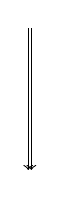
\begin{tikzpicture}\draw[->] (0,1.8)--(0,0);\draw[->] (.04,1.8)--(.04,0);\end{tikzpicture}}}
Noter qu'alors aussi
\[
\begin{aligned}
\underline{\mathrm{Hom}}_B(X,Y^M)&\simeq p_{A*}\underbrace{\underline{\mathrm{Hom}}(X,\underline{\mathrm{Hom}}(p_A^*(M),Y))}\\
&\simeq p_{A*}(\underline{\mathrm{Hom}}(X\times p_A^*(M),Y))\\
&\simeq\mathrm{Hom}_B(X\times p_A^*(M),Y).
\end{aligned}
\]
\margin{\(^{*}\) Pour \unsure{construire|avoir} \(p_A^*(M)\), il faudrait que \(\forall b\in\unsure{M|B}\) \inserted{\unsure{(pour b donné)}}, le foncteur \uline{constant} sur \(A\) de valeur \(M(b)\) soit représentable. Mais cela signifie que \(M(b)\) est réduit à \unsure{un élém.|un élément} et \(A\) a \unsure{objt} final. Donc \unsure{OK ssi} \(M\) objet final de \(\widehat B\), et \(A\) admet objet final !!}
\mspage{7}

\scanpage{9}
\figure{\begin{tikzpicture}[x=.075cm,y=.16cm]
\node[anchor=base west,inner sep=0pt,font=\tiny\ttfamily] at (0,0) {end};
\node[anchor=base west,inner sep=0pt,font=\tiny\ttfamily] at (0,-1) {disp\ cray1};
\node[anchor=base west,inner sep=0pt,font=\tiny\ttfamily] at (0,-2) {//PREDONTA\ JOB\ CNU0000-PREDONT,MSGCLASS=A,TYPRUN=UIC};
\node[anchor=base west,inner sep=0pt,font=\tiny\ttfamily] at (0,-3) {/*JOB=PREDONTA,ACCT=Y62200301};
\node[anchor=base west,inner sep=0pt,font=\tiny\ttfamily] at (0,-4) {//PREDONTA\ JOB\ MSGLEVEL=(1,1)};
\node[anchor=base west,inner sep=0pt,font=\tiny\ttfamily] at (0,-5) {//\ \ \ \ \ \ \ \ \ \ EXEC\ CSSBATCH};
\node[anchor=base west,inner sep=0pt,font=\tiny\ttfamily] at (0,-6) {//CRAYIN\ \ \ \ DD\ *};
\node[anchor=base west,inner sep=0pt,font=\tiny\ttfamily] at (0,-7) {JOB,JN=PREDONTA,T=9,TIO=9.};
\node[anchor=base west,inner sep=0pt,font=\tiny\ttfamily] at (0,-8) {CFT.};
\node[anchor=base west,inner sep=0pt,font=\tiny\ttfamily] at (0,-9) {LDR.};
\node[anchor=base west,inner sep=0pt,font=\tiny\ttfamily] at (0,-10) {/EOF};
\node[anchor=base west,inner sep=0pt,font=\tiny\ttfamily] at (0,-11) {\ \ \ \ \ \ PROGRAM\ GUTS};
\node[anchor=base west,inner sep=0pt,font=\tiny\ttfamily] at (0,-12) {\ \ \ \ \ \ WRITE(6,1)};
\node[anchor=base west,inner sep=0pt,font=\tiny\ttfamily] at (0,-13) {\ \ \ \ 1\ FORMAT('\ BONJOUR')};
\node[anchor=base west,inner sep=0pt,font=\tiny\ttfamily] at (0,-14) {\ \ \ \ \ \ STOP};
\node[anchor=base west,inner sep=0pt,font=\tiny\ttfamily] at (0,-15) {\ \ \ \ \ \ END};
\node[anchor=base west,inner sep=0pt,font=\tiny\ttfamily] at (0,-16) {/*};
\node[anchor=base west,inner sep=0pt,font=\tiny\ttfamily] at (0,-17) {//};
\node[anchor=base west,inner sep=0pt,font=\tiny\ttfamily] at (0,-18) {205\ //\ \ \ \ \ space=(trk,(180,0,35),rlse)};
\node[anchor=base west,inner sep=0pt,font=\tiny\ttfamily] at (0,-19) {l\ modulconv};
\node[anchor=base west,inner sep=0pt,font=\tiny\ttfamily] at (0,-20) {00010\ //PREDONTA\ JOB\ CNU0049\#NODER-PREDONT,\deleted{CLASS=R,TIME=(0,3)}};
\node[anchor=base west,inner sep=0pt,font=\tiny\ttfamily] at (0,-21) {00020\ //JOBLIB\ DD\ DSN=CNU2.MODULEF.UTIA,DISP=SHR};
\node[anchor=base west,inner sep=0pt,font=\tiny\ttfamily] at (0,-22) {00030\ //ETAP1\ EXEC\ PGM=FLIPFLOP};
\node[anchor=base west,inner sep=0pt,font=\tiny\ttfamily] at (0,-23) {00040\ //SYSUT1\ DD\ DSN=CNU1.MODULEF.V33.INTERME1(MEFCOSDS),DISP=(OLD,PASS)};
\node[anchor=base west,inner sep=0pt,font=\tiny\ttfamily] at (0,-24) {00050\ //SYSUT2\ DD\ DSN=\&AUX,SPACE=(TRK,180),UNIT=SYSDA,DISP=(,PASS),};
\node[anchor=base west,inner sep=0pt,font=\tiny\ttfamily] at (0,-25) {00060\ //\ DCB=(RECFM=F,LRECL=80,BLKSIZE=80)};
\node[anchor=base west,inner sep=0pt,font=\tiny\ttfamily] at (0,-26) {00070\ //ETAP2\ EXEC\ PGM=UPDATE,PARM=NEW,COND=(0,NE,ETAP1)};
\node[anchor=base west,inner sep=0pt,font=\tiny\ttfamily] at (0,-27) {00080\ //SYSPRINT\ DD\ DUMMY};
\node[anchor=base west,inner sep=0pt,font=\tiny\ttfamily] at (0,-28) {00090\ //SYSIN\ DD\ DSN=\&AUX,DISP=(OLD,DELETE)};
\node[anchor=base west,inner sep=0pt,font=\tiny\ttfamily] at (0,-29) {00100\ //SYSIN2\ DD\ UNIT=SYSDA,SPACE=(CYL,\deleted{\unsure{4}}\inserted{6})};
\node[anchor=base west,inner sep=0pt,font=\tiny\ttfamily] at (0,-30) {00110\ //SYSUT2\ DD\ DSN=CNU2.MODULEF.COSDS,};
\node[anchor=base west,inner sep=0pt,font=\tiny\ttfamily] at (0,-31) {00120\ //\ UNIT=SYSDA,DISP=(,CATLG,DELETE),SPACE=(TRK,(180,0,35),RLSE),};
\node[anchor=base west,inner sep=0pt,font=\tiny\ttfamily] at (0,-32) {00130\ //\ VOL=SER=\unsure{SYSPPP|SYSPFP},DCB=(RECFM=FB,LRECL=80,BLKSIZE=19040)};
\node[anchor=base west,inner sep=0pt,font=\tiny\ttfamily] at (0,-33) {00140\ //};

\node[anchor=base west] at (-5,-20) {$(\ast$};
\draw[->,thick] (-2.5,-20)--(-.5,-20);
\node[anchor=base west] at (47,-18.8) {\inserted{REGION}};
\draw (53,-23) ellipse (3,.65);
\draw (34,-30) ellipse (3,.65);
\draw[->,thick] (-2.8,-29)--(-.5,-29);
\draw[->,thick] (-2.8,-33)--(-.5,-33);
\draw (1,-33.2)--(3,-32.6)--(3,-33.4) (5,-33.3)--(7,-32.8)--(7,-33.5) (8,-33.5)--(10,-33.0);
\end{tikzpicture}}
\mspage{8}

\scanpage{10}
\mspage{d}
donc
\[
\underline{\mathrm{Hom}}_B(X,Y^M)\simeq\underline{\mathrm{Hom}}_B(\underbrace{X\times p_A^*(M)}_{\deleted{\unsure{\mathop{=}\limits^{\mathrm{déf}}}X\otimes\unsure{M}}},Y).
\]
\unsure{Relation} valable pour tt $X,Y\in(A\times B)^\wedge$, \unsure{mais nous|mais ici}, nous nous \unsure{intéressons} à cette formule pour $X,Y\in\underline{\mathrm{Hom}}(B^o,A)$, en nous attendant à y trouver aussi $Y^M,X\otimes M$ dans $\underline{\mathrm{Hom}}(B^o,A)$. On a vu des conditions naturelles pour qu'il en soit ainsi pour $Y^M$ (existence de certaines $\varprojlim$ dans $A$, à l'exclusion des $\underline{\mathrm{Hom}}$ internes dans $A$),

Il reste à regarder pour $X\times p_A^*(M)$, qui en tant que foncteur $B^o\mathbin{\text{---}}\widehat A$ s'identifie à
\[
b\longmapsto\underbrace{X(b)\times M(b)}=\bigl\{a\longmapsto\deleted{X}\underbrace{\mathrm{Hom}_A(a,X(b))}_{X(b)(a)=X(a,b)}\times M(b)\bigr).
\]
Comme \unsure{tantôt|d'hab.}, il n'est pratiquement jamais représentable. Mais supposons que dans $A$ les sommes existent (\unsure{les sommes} finies suffisent si les $M(b)$ sont eux-mêmes finis) et définissons
\[
X\otimes M\in\underline{\mathrm{Hom}}(B^o,A)\quad\text{par}
\]
\[
\deleted{(X\otimes M)(b)}=\deleted{\unsure{X(b)}}\underset{\sigma\in M(b)}{\coprod_A}\underbrace{X(b)}
\]
\margin{\diagram{\begin{tikzcd}[column sep=large]
(\phantom{X} \arrow[r,"\unsure{non}","\mathrm{iso}"',"\sim" description] & \displaystyle\underset{\sigma\in M(b)}{\coprod_{\widehat A}}X(b) \\
& {}=(X\times p_A^*(M))(b)
\end{tikzcd}}}
alors on a, pour $X_{\deleted{\unsure{b}}},Y$ dans $\underline{\mathrm{Hom}}(B^o,A)$
\[
\underline{\mathrm{Hom}}_B(X,Y^M)\simeq\underline{\mathrm{Hom}}_B(X\otimes M,Y)\qquad\text{trifonctoriel}
\]
\mspage{9}

\scanpage{11}
\figure{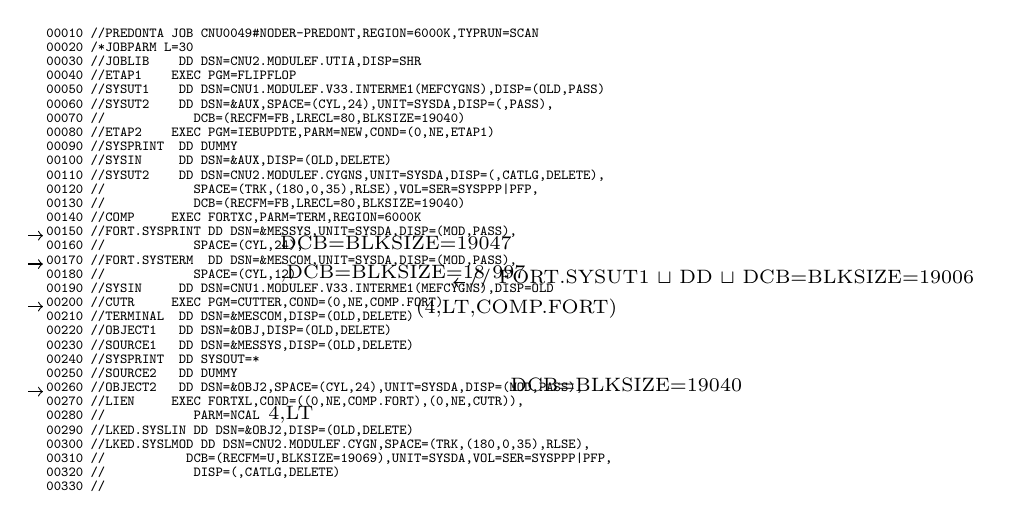
\begin{tikzpicture}[x=.075cm,y=.18cm]
\node[anchor=base west,inner sep=0pt,font=\tiny\ttfamily] at (0,0) {00010\ //PREDONTA\ JOB\ CNU0049\#NODER-PREDONT,REGION=6000K,TYPRUN=SCAN};
\node[anchor=base west,inner sep=0pt,font=\tiny\ttfamily] at (0,-1) {00020\ /*JOBPARM\ L=30};
\node[anchor=base west,inner sep=0pt,font=\tiny\ttfamily] at (0,-2) {00030\ //JOBLIB\ \ \ \ DD\ DSN=CNU2.MODULEF.UTIA,DISP=SHR};
\node[anchor=base west,inner sep=0pt,font=\tiny\ttfamily] at (0,-3) {00040\ //ETAP1\ \ \ \ EXEC\ PGM=FLIPFLOP};
\node[anchor=base west,inner sep=0pt,font=\tiny\ttfamily] at (0,-4) {00050\ //SYSUT1\ \ \ \ DD\ DSN=CNU1.MODULEF.V33.INTERME1(MEFCYGNS),DISP=(OLD,PASS)};
\node[anchor=base west,inner sep=0pt,font=\tiny\ttfamily] at (0,-5) {00060\ //SYSUT2\ \ \ \ DD\ DSN=\&AUX,SPACE=(CYL,24),UNIT=SYSDA,DISP=(,PASS),};
\node[anchor=base west,inner sep=0pt,font=\tiny\ttfamily] at (0,-6) {00070\ //\ \ \ \ \ \ \ \ \ \ \ \ DCB=(RECFM=FB,LRECL=80,BLKSIZE=19040)};
\node[anchor=base west,inner sep=0pt,font=\tiny\ttfamily] at (0,-7) {00080\ //ETAP2\ \ \ \ EXEC\ PGM=IEBUPDTE,PARM=NEW,COND=(0,NE,ETAP1)};
\node[anchor=base west,inner sep=0pt,font=\tiny\ttfamily] at (0,-8) {00090\ //SYSPRINT\ \ DD\ DUMMY};
\node[anchor=base west,inner sep=0pt,font=\tiny\ttfamily] at (0,-9) {00100\ //SYSIN\ \ \ \ \ DD\ DSN=\&AUX,DISP=(OLD,DELETE)};
\node[anchor=base west,inner sep=0pt,font=\tiny\ttfamily] at (0,-10) {00110\ //SYSUT2\ \ \ \ DD\ DSN=CNU2.MODULEF.CYGNS,UNIT=SYSDA,DISP=(,CATLG,DELETE),};
\node[anchor=base west,inner sep=0pt,font=\tiny\ttfamily] at (0,-11) {00120\ //\ \ \ \ \ \ \ \ \ \ \ \ SPACE=(TRK,(180,0,35),RLSE),VOL=SER=SYS\unsure{PPP|PFP},};
\node[anchor=base west,inner sep=0pt,font=\tiny\ttfamily] at (0,-12) {00130\ //\ \ \ \ \ \ \ \ \ \ \ \ DCB=(RECFM=FB,LRECL=80,BLKSIZE=19040)};
\node[anchor=base west,inner sep=0pt,font=\tiny\ttfamily] at (0,-13) {00140\ //COMP\ \ \ \ \ EXEC\ FORTXC,PARM=TERM,REGION=6000K};
\node[anchor=base west,inner sep=0pt,font=\tiny\ttfamily] at (0,-14) {00150\ //FORT.SYSPRINT\ DD\ DSN=\&MESSYS,UNIT=SYSDA,DISP=(MOD,PASS),};
\node[anchor=base west,inner sep=0pt,font=\tiny\ttfamily] at (0,-15) {00160\ //\ \ \ \ \ \ \ \ \ \ \ \ SPACE=(CYL,24),};
\node[anchor=base west,inner sep=0pt,font=\tiny\ttfamily] at (0,-16) {00170\ //FORT.SYSTERM\ \ DD\ DSN=\&MESCOM,UNIT=SYSDA,DISP=(MOD,PASS),};
\node[anchor=base west,inner sep=0pt,font=\tiny\ttfamily] at (0,-17) {00180\ //\ \ \ \ \ \ \ \ \ \ \ \ SPACE=(CYL,12)};
\node[anchor=base west,inner sep=0pt,font=\tiny\ttfamily] at (0,-18) {00190\ //SYSIN\ \ \ \ \ DD\ DSN=CNU1.MODULEF.V33.INTERME1(MEFCYGNS),DISP=OLD};
\node[anchor=base west,inner sep=0pt,font=\tiny\ttfamily] at (0,-19) {00200\ //CUTR\ \ \ \ \ EXEC\ PGM=CUTTER,COND=(0,NE,COMP.FORT)};
\node[anchor=base west,inner sep=0pt,font=\tiny\ttfamily] at (0,-20) {00210\ //TERMINAL\ \ DD\ DSN=\&MESCOM,DISP=(OLD,DELETE)};
\node[anchor=base west,inner sep=0pt,font=\tiny\ttfamily] at (0,-21) {00220\ //OBJECT1\ \ \ DD\ DSN=\&OBJ,DISP=(OLD,DELETE)};
\node[anchor=base west,inner sep=0pt,font=\tiny\ttfamily] at (0,-22) {00230\ //SOURCE1\ \ \ DD\ DSN=\&MESSYS,DISP=(OLD,DELETE)};
\node[anchor=base west,inner sep=0pt,font=\tiny\ttfamily] at (0,-23) {00240\ //SYSPRINT\ \ DD\ SYSOUT=*};
\node[anchor=base west,inner sep=0pt,font=\tiny\ttfamily] at (0,-24) {00250\ //SOURCE2\ \ \ DD\ DUMMY};
\node[anchor=base west,inner sep=0pt,font=\tiny\ttfamily] at (0,-25) {00260\ //OBJECT2\ \ \ DD\ DSN=\&OBJ2,SPACE=(CYL,24),UNIT=SYSDA,DISP=(MOD,PASS),};
\node[anchor=base west,inner sep=0pt,font=\tiny\ttfamily] at (0,-26) {00270\ //LIEN\ \ \ \ \ EXEC\ FORTXL,COND=((\deleted{0,NE},COMP.FORT),(0,NE,CUTR)),};
\node[anchor=base west,inner sep=0pt,font=\tiny\ttfamily] at (0,-27) {00280\ //\ \ \ \ \ \ \ \ \ \ \ \ PARM=NCAL};
\node[anchor=base west,inner sep=0pt,font=\tiny\ttfamily] at (0,-28) {00290\ //LKED.SYSLIN\ DD\ DSN=\&OBJ2,DISP=(OLD,DELETE)};
\node[anchor=base west,inner sep=0pt,font=\tiny\ttfamily] at (0,-29) {00300\ //LKED.SYSLMOD\ DD\ DSN=CNU2.MODULEF.CYGN,SPACE=(TRK,(180,0,35),RLSE),};
\node[anchor=base west,inner sep=0pt,font=\tiny\ttfamily] at (0,-30) {00310\ //\ \ \ \ \ \ \ \ \ \ \ DCB=(RECFM=U,BLKSIZE=19069),UNIT=SYSDA,VOL=SER=SYS\unsure{PPP|PFP},};
\node[anchor=base west,inner sep=0pt,font=\tiny\ttfamily] at (0,-31) {00320\ //\ \ \ \ \ \ \ \ \ \ \ \ DISP=(,CATLG,DELETE)};
\node[anchor=base west,inner sep=0pt,font=\tiny\ttfamily] at (0,-32) {00330\ //};

\draw[->] (-3,-14)--(-.5,-14);
\draw[->] (-3,-16)--(-.5,-16);
\draw[->] (-3,-19)--(-.5,-19);
\draw[->] (-3,-25)--(-.5,-25);
\node[anchor=base west,font=\scriptsize] at (38,-15) {\inserted{DCB=BLKSIZE=19047}};
\node[anchor=base west,font=\scriptsize] at (38,-17) {\inserted{,DCB=BLKSIZE=18 997}};
\node[anchor=base west,font=\scriptsize] at (70,-17.4) {\inserted{// FORT.SYSUT1 $\unsure{\sqcup}$ DD $\unsure{\sqcup}$ DCB=BLKSIZE=19006}};
\draw[<-] (69,-17.3)--(71,-17.3);
\node[anchor=base west,font=\scriptsize] at (61,-19.5) {\inserted{(4,LT,COMP.FORT)}};
\node[anchor=base west,font=\scriptsize] at (77,-25) {\inserted{DCB=BLKSIZE=19040}};
\node[anchor=base west,font=\scriptsize] at (36,-27) {\inserted{4,LT}};
\end{tikzpicture}}
\mspage{10}

\scanpage{12}
\mspage{e}
\diagram{\begin{tikzcd}
& (A\times B)^\wedge \arrow[dl,"p_{B*}"'] \arrow[dr,"p_{A*}"] & \\
\widehat A \arrow[ur,bend left=55,"p_B^*"] \arrow[dr,"q_{A*}=\Gamma_A"'] && \widehat B \arrow[ul,bend right=55,"p_A^*"'] \arrow[dl,"q_{B*}=\Gamma_B"] \\
& (\mathrm{Ens}) &
\end{tikzcd}}
\margin{\uline{\unsure{Récapitulation|Récapitulat$^\circ$}}}
\[
\begin{aligned}
X(a,b)&=\unsure{\Gamma|E}_{A\times B}\mathrm{Hom}(\overbrace{p_B^*(a)}^{\text{identifié à }\unsure{{}^g a}}\times\overbrace{p_A^*(b)}^{\text{identifié à }{}^d b},X)\\
&=\Gamma_{A\times B}(\underline{\mathrm{Hom}}_{A\times B}(\deleted{\unsure{p_B^*}}a\boxtimes b,X))
\end{aligned}
\quad\left\{\begin{aligned}&=\Gamma_A p_{B*}\underline{\mathrm{Hom}}\\&=\Gamma_B p_{A*}\underline{\mathrm{Hom}}\end{aligned}\right.
\]
\[
\deleted{\unsure{\simeq}}
\]
\[
{}^gX(a)=p_{\unsure{A|B}*}\underline{\mathrm{Hom}}_{A\times B}({}^ga,X)
\]
\[
{}^dX(b)=p_{B*}\underline{\mathrm{Hom}}_{A\times B}({}^db,X)
\]
\[
\deleted{\mathrm{Hom}(L\boxtimes M,X)=X(L,M)}
\]
\[
\begin{aligned}
X(L,M)&=\mathrm{Hom}_{A\times B}(L\boxtimes M,X)\\
&=\Gamma_{A\times B}\underline{\mathrm{Hom}}(L\boxtimes M,\unsure{Y|X})
\end{aligned}
\]
\[
{}^gX(L)=p_{A*}\underline{\mathrm{Hom}}_{A\times B}({}^gL,X)=\underline{\mathrm{Hom}}_B({}^gL,X)
\]
\[
{}^dX(M)=p_{\unsure{B|A}*}\underbrace{\underline{\mathrm{Hom}}_{A\times B}({}^dM,X)}_{X^M}=\underline{\mathrm{Hom}}_A({}^dM,X)
\]
\[
\underline{\mathrm{Hom}}_B(X,Y^M)\simeq\underline{\mathrm{Hom}}_B(X\otimes M,Y)
\]
\mspage{11}

\scanpage{13}
\figure{\begin{tikzpicture}[x=.075cm,y=.18cm]
\node[anchor=base west,inner sep=0pt,font=\tiny\ttfamily] at (0,0) {00010\ //PREDONTA\ JOB\ CNU0049\#NODER-PREDONT,REGION=1500K,TYPRUN=SCAN};
\node[anchor=base west,inner sep=0pt,font=\tiny\ttfamily] at (0,-1) {00020\ /*JOBPARM\ L=30};
\node[anchor=base west,inner sep=0pt,font=\tiny\ttfamily] at (0,-2) {00030\ //JOBLIB\ DD\ DSN=CNU2.MODULEF.UTIA,DISP=SHR};
\node[anchor=base west,inner sep=0pt,font=\tiny\ttfamily] at (0,-3) {00040\ //ETAP1\ EXEC\ PGM=FLIPFLOP};
\node[anchor=base west,inner sep=0pt,font=\tiny\ttfamily] at (0,-4) {00050\ //SYSUT1\ DD\ DSN=CNU1.MODULEF.V33.INTERME1(MEFCOSDS),DISP=(OLD,PASS)};
\node[anchor=base west,inner sep=0pt,font=\tiny\ttfamily] at (0,-5) {00060\ //SYSUT2\ DD\ DSN=\&AUX,SPACE=(CYL,6),UNIT=SYSDA,DISP=(,PASS),};
\node[anchor=base west,inner sep=0pt,font=\tiny\ttfamily] at (0,-6) {00070\ //\ DCB=(RECFM=F,LRECL=80,BLKSIZE=80)};
\node[anchor=base west,inner sep=0pt,font=\tiny\ttfamily] at (0,-7) {00080\ //ETAP2\ EXEC\ PGM=UPDATE,PARM=NEW,COND=(0,NE,ETAP1)};
\node[anchor=base west,inner sep=0pt,font=\tiny\ttfamily] at (0,-8) {00090\ //SYSPRINT\ DD\ DUMMY};
\node[anchor=base west,inner sep=0pt,font=\tiny\ttfamily] at (0,-9) {00100\ //SYSIN\ DD\ DSN=\&AUX,DISP=(OLD,DELETE)};
\node[anchor=base west,inner sep=0pt,font=\tiny\ttfamily] at (0,-10) {00110\ //SYSIN2\ DD\ UNIT=SYSDA,SPACE=(CYL,6)};
\node[anchor=base west,inner sep=0pt,font=\tiny\ttfamily] at (0,-11) {00120\ //SYSUT2\ DD\ DSN=CNU2.MODULEF.COSDS,};
\node[anchor=base west,inner sep=0pt,font=\tiny\ttfamily] at (0,-12) {00130\ //\ UNIT=SYSDA,DISP=(,CATLG,DELETE),SPACE=(TRK,(180,0,35),RLSE),};
\node[anchor=base west,inner sep=0pt,font=\tiny\ttfamily] at (0,-13) {00140\ //\ VOL=SER=SYS\unsure{PPP|PFP},DCB=(RECFM=FB,LRECL=80,BLKSIZE=19040)};
\node[anchor=base west,inner sep=0pt,font=\tiny\ttfamily] at (0,-14) {00150\ //COMP\ \ \ \ \ \ \ EXEC\ FORTXC,PARM=TERM,REGION=500K,\deleted{COND=EVEN}};
\node[anchor=base west,inner sep=0pt,font=\tiny\ttfamily] at (0,-15) {00160\ //FORT.SYSPRINT\ DD\ DSN=\&MESSYS,SPACE=(CYL,6),UNIT=SYSDA,DISP=(MOD,PASS)};
\node[anchor=base west,inner sep=0pt,font=\tiny\ttfamily] at (0,-16) {00170\ //FORT.SYSTERM\ \ DD\ DSN=\&MESCOM,SPACE=(CYL,\deleted{\unsure{3}}\inserted{2}),UNIT=SYSDA,DISP=(MOD,PASS)};
\node[anchor=base west,inner sep=0pt,font=\tiny\ttfamily] at (0,-17) {00180\ //SYSIN\ \ \ \ DD\ DSN=CNU1.MODULEF.V33.INTERME1(MEFCOSDS),DISP=OLD};
\node[anchor=base west,inner sep=0pt,font=\tiny\ttfamily] at (0,-18) {00190\ //CUTR\ \ \ \ EXEC\ PGM=CUTTER,COND=((0,NE,COMP.FORT),\deleted{EVEN})};
\node[anchor=base west,inner sep=0pt,font=\tiny\ttfamily] at (0,-19) {00200\ //TERMINAL\ DD\ DSN=\&MESCOM,DISP=(OLD,DELETE)};
\node[anchor=base west,inner sep=0pt,font=\tiny\ttfamily] at (0,-20) {00210\ //OBJECT1\ \ DD\ DSN=\&OBJ,DISP=(OLD,DELETE)};
\node[anchor=base west,inner sep=0pt,font=\tiny\ttfamily] at (0,-21) {00220\ //SOURCE1\ \ DD\ DSN=\&MESSYS,DISP=(OLD,DELETE)};
\node[anchor=base west,inner sep=0pt,font=\tiny\ttfamily] at (0,-22) {00230\ //SYSPRINT\ DD\ SYSOUT=*};
\node[anchor=base west,inner sep=0pt,font=\tiny\ttfamily] at (0,-23) {00240\ //SOURCE2\ \ DD\ DUMMY};
\node[anchor=base west,inner sep=0pt,font=\tiny\ttfamily] at (0,-24) {00250\ //OBJECT2\ \ DD\ DSN=\&OBJ2,SPACE=(CYL,6),UNIT=SYSDA,DISP=(MOD,PASS)};
\node[anchor=base west,inner sep=0pt,font=\tiny\ttfamily] at (0,-25) {00260\ //LIEN\ \ \ \ \ \ \ EXEC\ FORTXL,COND=((0,NE,COMP.FORT),(0,NE,CUTR),\deleted{EVEN}),};
\node[anchor=base west,inner sep=0pt,font=\tiny\ttfamily] at (0,-26) {00270\ //\ \ \ \ \ \ \ \ \ \ \ \ PARM=NCAL};
\node[anchor=base west,inner sep=0pt,font=\tiny\ttfamily] at (0,-27) {00280\ //LKED.SYSLIN\ \ DD\ DSN=\&OBJ2,DISP=(OLD,DELETE)};
\node[anchor=base west,inner sep=0pt,font=\tiny\ttfamily] at (0,-28) {00290\ //LKED.SYSLMOD\ DD\ DSN=CNU2.MODULEF.COSD,SPACE=(TRK,(180,0,35),RLSE),};
\node[anchor=base west,inner sep=0pt,font=\tiny\ttfamily] at (0,-29) {00300\ //\ \ DCB=(RECFM=U,BLKSIZE=19040),UNIT=SYSDA,VOL=SER=SYS\unsure{PPP|PFP},DISP=(,CATLG\deleted{)}\inserted{,DELETE)}};
\node[anchor=base west,inner sep=0pt,font=\tiny\ttfamily] at (0,-30) {00310\ //};
\draw[->,thick] (-3,-5)--(-.5,-5);
\draw[->,thick] (-3,-10)--(-.5,-10);
\draw[->,thick] (-3,-14)--(-.5,-14);
\draw[->,thick] (-3,-15)--(-.5,-15);
\draw[->,thick] (-3,-18)--(-.5,-18);
\draw[->,thick] (-3,-24)--(-.5,-24);
\draw[->,thick] (-3,-25)--(-.5,-25);
\draw (-1,-2.6)--(66,-2.6);
\draw (-1,-6.6)--(74,-6.6);
\draw (-1,-13.6)--(69,-13.6);
\draw (-1,-17.6)--(77,-17.6);
\draw (-1,-24.6)--(85,-24.6);

\draw (38,-5) ellipse (1.4,.8);
\draw (39.5,-10) ellipse (1.2,.85);
\draw (48,-15) ellipse (1.5,.9);
\draw (41,-24) ellipse (1.4,1.05);
\node[anchor=base west,font=\scriptsize] at (42,-22.8) {\inserted{24}};
\end{tikzpicture}}
\mspage{12}

\scanpage{14}
\mspage{f}
\[
\begin{aligned}
(A\times B)^\wedge&\mathop{=}\limits^{\mathrm{déf}}\underline{\mathrm{Hom}}((A\times B)^o,(\mathrm{Ens}))\simeq\underline{\mathrm{Hom}}(A^o\times B^o,(\mathrm{Ens}))\\
&\simeq\underline{\mathrm{Hom}}(A^o,\deleted{\mathrm{Ens}}\inserted{\widehat B})\simeq\underline{\mathrm{Hom}}_!(\widehat A^o,\deleted{\unsure{\mathrm{Ens}\,\widehat A}}\inserted{\widehat B})\\
&\simeq\underline{\mathrm{Hom}}(B^o,\widehat A)\simeq\underline{\mathrm{Hom}}_!(\widehat B^o,\widehat A)\\
&\simeq\underline{\mathrm{Hom}}_{!!}((\widehat A)^o\times(\widehat B)^o,\mathrm{Ens})\simeq\underline{\mathrm{Hom}}_!((\widehat A\times\widehat B)^o,\mathrm{Ens})
\end{aligned}
\]
\margin{le signe $!$ signifie : foncteurs commutant aux $\varprojlim$ quelconques ! le signe $!!$ a le sens analogue pour \uline{chacune} des variables séparément (\unsure{mais est équiv.} à un seul signe $!$ relatif à $(\widehat A\times\widehat B)^o$)}
\figure{\begin{tikzpicture}\draw (0,0)--(0,1.7);\end{tikzpicture}}
Si $X\in(A\times B)^\wedge$, le foncteur \deleted{\unsure{qui}} correspondant
\[
(\unsure{L|X},M)\longmapsto X(L,M):\underset{(\widehat A\times\widehat B)^o}{\underbrace{\widehat A^o\times\widehat B^o}}\mathbin{\unsure{\text{---}|\longrightarrow}}(\mathrm{Ens})
\]
est donné par
\[
X(L,M)=\mathrm{Hom}(L\boxtimes M,X)\deleted{=\unsure{\mathrm{Hom}}}\quad\text{où}\quad L\boxtimes M=p_B^*(L)\boxtimes p_A^*(M).
\]
\deleted{\uline{Corollaire}}\inserted{\uline{Proposition}} Le foncteur $(L,M)\longmapsto L\boxtimes M$ de $(\widehat A\times\widehat B)^o$ dans $\deleted{\unsure{(A\times B)^\wedge|(\widehat A\times\widehat B)^\wedge}}\inserted{(\widehat A\times\widehat B)^\wedge}$ est pleinement fidèle, il s'identifie au foncteur qui associe à tout \unsure{élém.} $(L,M)$ de $\widehat A\times\widehat B$ le foncteur
\deleted{\unsure{can.}\diagram{\begin{tikzcd}
(\widehat A\times\widehat B)^o\arrow[r] & \underline{\mathrm{Hom}}((\widehat A\times\widehat B)^o,
\end{tikzcd}}}
\unsure{contravariant} \deleted{\unsure{considéré qu'il représente}} sur $\widehat A\times\widehat B$ qu'il représente
\[
(L\boxtimes M)(L',M')\simeq\mathrm{Hom}_{\widehat A\times\widehat B}((L',M'),(L,M))=\mathrm{Hom}(L',L)\times\mathrm{Hom}(M',M)
\]
\margin{\unsure{Hom-}}
\[
\mathrm{Hom}(L'\boxtimes M',L^{\unsure{*}}\boxtimes M)
\]
En effet, la formule est vraie par définition de $L\boxtimes M$ si \deleted{\unsure{L'\in A}}

\deleted{Bien sûr, par fonctorialité, on a}
\deleted{\diagram{\begin{tikzcd}[column sep=large]
\mathrm{Hom}(L',L)\times\mathrm{Hom}(M',M)\arrow[r] & \mathrm{Hom}(L'\boxtimes M',L\boxtimes M)
\end{tikzcd}}}
$L'=a\in\mathrm{Ob}\,A$, $M'=b\in\mathrm{Ob}\,B$, \deleted{\unsure{et le}} D'autre part, pour $L,M$ fixés, et $L',M'$ variables, \unsure{les deux mbs}, comme fonctions de $L',M'$, transforment $\varinjlim$ en $\varprojlim$
\deleted{\unsure{ce qui est le cas}} \deleted{\unsure{et il paraît que}}
--- d'où la conclusion.

\uline{Corollaire}
\[
\underline{\mathrm{Hom}}(L'\boxtimes M',\deleted{\unsure{M}}L\boxtimes M)\simeq\underline{\mathrm{Hom}}(L',L)\boxtimes\underline{\mathrm{Hom}}(M',M)
\]
\uline{Dém.} Il suffit de prendre les $\mathrm{Hom}(a\boxtimes b,-)$, pour $(a,b)\in\mathrm{Ob}\,A\times B$
\[
\begin{array}{ll}
\Vert&\Vert\\
\mathrm{Hom}_{A\times B}(\underbrace{\deleted{a\times L'\boxtimes M'}\inserted{(a\boxtimes b)\times(L'\boxtimes M')}}_{(a\times L')\boxtimes(b\times M')},L\boxtimes M)&\mathrm{Hom}_A(a,\underline{\mathrm{Hom}}(L',L))\times\mathrm{Hom}_B(b,\underline{\mathrm{Hom}}(M',M))\\
\Vert&\Vert\\
\mathrm{Hom}_A(a\times L',L)\times\mathrm{Hom}_B(b\times M',M)&\mathrm{Hom}_A(a\times L',L)\times\mathrm{Hom}_B(b\times M',M)
\end{array}
\]
\margin{OK}
\mspage{13}

\scanpage{15}
\[
(X^{\Delta_n})_0=\deleted{\underline{\operatorname{Hom}}}_B p_{B*}(\underline{\operatorname{Hom}}(p_A^*(\Delta_n),X))=X_n
\]
\[
(X^{\dot\Delta_n})_0=p_{B*}\underline{\operatorname{Hom}}(\dot\Delta_n,X)=\varprojlim(X_{n-1},X_{n-2})
\]
\diagram{\begin{tikzcd}X^{\Delta_n}\arrow[r]&X^{\dot\Delta_n}\times_{Y^{\dot\Delta_n}}Y^{\Delta_n}\end{tikzcd}}
\margin{$(\operatorname{cosk}_{n-1}X)_n\deleted{\unsure{X_2}}$}
\figure{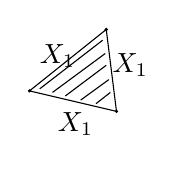
\begin{tikzpicture}[scale=.65]
\draw (0,0)--(1.5,1.2)--(1.7,-.4)--cycle;
\fill (0,0) circle(1pt);\fill(1.5,1.2)circle(1pt);\fill(1.7,-.4)circle(1pt);
\draw (.2,.04)--(1.43,.99) (.45,-.03)--(1.48,.73) (.7,-.1)--(1.5,.5) (1,-.18)--(1.55,.22) (1.3,-.25)--(1.58,-.03);
\node at(.55,.68){$X_1$};\node at(1.97,.5){$X_1$};\node at(.9,-.65){$X_1$};
\end{tikzpicture}}
\diagram{\begin{tikzcd}X_n\arrow[r]&(X^{\dot\Delta_n})_0\times_{(Y^{\dot\Delta_n})_0}Y_n\end{tikzcd}}
\margin{$A_n=A$\par $A$}
\diagram{\begin{tikzcd}X_{n-2}\arrow[r,no head,shift left=3]\arrow[r,no head]\arrow[r,no head,shift right=3]&X_{n-1}\end{tikzcd}}
\[\underline{\operatorname{Hom}}(\dot\Delta_n,a)\]
\diagram{\begin{tikzcd}\underline{\operatorname{Hom}}(M,a)\arrow[r,Rightarrow,"??"]&a\end{tikzcd}}
\[\operatorname{Hom}(X\times M,a)\simeq\operatorname{Hom}(X,-)\]
\[\operatorname{Hom}(\alpha\boxtimes(\beta\times M),\deleted{a}\unsure{a}\boxtimes e_B)\simeq\operatorname{Hom}(\alpha\boxtimes\beta,a\boxtimes\unsure{e_B}\]
\[\operatorname{Hom}\]
\[L\]
\figure{\begin{tikzpicture}[x=.075cm,y=.22cm]
\node[anchor=base west,inner sep=0pt,font=\tiny\ttfamily] at (0,0) {00040\ //ETAP1\ EXEC\ PGM=FLIPFLOP};
\node[anchor=base west,inner sep=0pt,font=\tiny\ttfamily] at (0,-1) {00050\ //SYSUT1\ DD\ DSN=CNU1.MODULEF.V33.INTERME1(MEFCOSDS),DISP=(OLD,PASS)};
\node[anchor=base west,inner sep=0pt,font=\tiny\ttfamily] at (0,-2) {00060\ //SYSUT2\ DD\ DSN=\&AUX,SPACE=(CYL,24),UNIT=SYSDA,DISP=(,PASS),};
\node[anchor=base west,inner sep=0pt,font=\tiny\ttfamily] at (0,-3) {00070\ //\ DCB=(RECFM=F\inserted{B},LRECL=80,BLKSIZE=\deleted{80}\inserted{19040})};
\node[anchor=base west,inner sep=0pt,font=\tiny\ttfamily] at (0,-4) {00080\ //ETAP2\ EXEC\ PGM=UPDATE,PARM=NEW,COND=(0,NE,ETAP1)};
\node[anchor=base west,inner sep=0pt,font=\tiny\ttfamily] at (0,-5) {00090\ //SYSPRINT\ DD\ DUMMY};
\node[anchor=base west,inner sep=0pt,font=\tiny\ttfamily] at (0,-6) {00100\ //SYSIN\ DD\ DSN=\&AUX,DISP=(OLD,DELETE)};
\node[anchor=base west,inner sep=0pt,font=\tiny\ttfamily] at (0,-7) {\deleted{00110\ //SYSIN2\ DD\ UNIT=SYSDA,SPACE=(CYL,24)}};
\node[anchor=base west,inner sep=0pt,font=\tiny\ttfamily] at (0,-8) {00120\ //SYSUT2\ DD\ DSN=CNU2.MODULEF.COSDS,};
\node[anchor=base west,inner sep=0pt,font=\tiny\ttfamily] at (0,-9) {00130\ //\ UNIT=SYSDA,DISP=(,CATLG,DELETE),SPACE=(TRK,(180,0,35),RLSE),};
\node[anchor=base west,inner sep=0pt,font=\tiny\ttfamily] at (0,-10) {00140\ //\ VOL=SER=SYS\unsure{PPP|PFP},DCB=(RECFM=FB,LRECL=80,BLKSIZE=19040)};
\node[anchor=base west,inner sep=0pt,font=\tiny\ttfamily] at (0,-11) {00150\ //COMP\ \ \ \ \ \ \ EXEC\ FORTXC,PARM=TERM,REGION=6000K};
\node[anchor=base west,inner sep=0pt,font=\tiny\ttfamily] at (0,-12) {00160\ //FORT.SYSPRINT\ DD\ DSN=\&MESSYS,UNIT=SYSDA,DISP=(MOD,PASS),};
\node[anchor=base west,inner sep=0pt,font=\tiny\ttfamily] at (0,-13) {00170\ //\ SPACE=(CYL,24)};
\node[anchor=base west,inner sep=0pt,font=\tiny\ttfamily] at (0,-14) {00180\ //FORT.SYSTERM\ DD\ DSN=\&MESCOM,UNIT=SYSDA,DISP=(MOD,PASS),};
\node[anchor=base west,inner sep=0pt,font=\tiny\ttfamily] at (0,-15) {00185\ //\ SPACE=(CYL,12)};
\node[anchor=base west,inner sep=0pt,font=\tiny\ttfamily] at (0,-16) {00190\ //SYSIN\ \ \ \ DD\ DSN=CNU1.MODULEF.V33.INTERME1(MEFCOSDS),DISP=OLD};
\node[anchor=base west,inner sep=0pt,font=\tiny\ttfamily] at (0,-17) {00200\ //CUTR\ \ \ \ EXEC\ PGM=CUTTER,COND=(0,NE,COMP.FORT)};
\node[anchor=base west,inner sep=0pt,font=\tiny\ttfamily] at (0,-18) {00210\ //TERMINAL\ DD\ DSN=\&MESCOM,DISP=(OLD,DELETE)};
\node[anchor=base west,inner sep=0pt,font=\tiny\ttfamily] at (0,-19) {00220\ //OBJECT1\ DD\ DSN=\&OBJ,DISP=(OLD,DELETE)};
\node[anchor=base west,inner sep=0pt,font=\tiny\ttfamily] at (0,-20) {00230\ //SOURCE1\ DD\ DSN=\&MESSYS,DISP=(OLD,DELETE)};
\node[anchor=base west,inner sep=0pt,font=\tiny\ttfamily] at (0,-21) {00240\ //SYSPRINT\ DD\ SYSOUT=*};
\node[anchor=base west,inner sep=0pt,font=\tiny\ttfamily] at (0,-22) {00250\ //SOURCE2\ DD\ DUMMY};
\node[anchor=base west,inner sep=0pt,font=\tiny\ttfamily] at (0,-23) {00260\ //OBJECT2\ DD\ DSN=\&OBJ2,SPACE=(CYL,24),UNIT=SYSDA,DISP=(MOD,PASS)};
\node[anchor=base west,inner sep=0pt,font=\tiny\ttfamily] at (0,-24) {00270\ //LIEN\ \ \ \ \ \ \ EXEC\ FORTXL,COND=((0,NE,COMP.FORT),(0,NE,CUTR)),};
\node[anchor=base west,inner sep=0pt,font=\tiny\ttfamily] at (0,-25) {00280\ //\ PARM=NCAL};
\node[anchor=base west,inner sep=0pt,font=\tiny\ttfamily] at (0,-26) {00290\ //LKED.SYSLIN\ DD\ DSN=\&OBJ2,DISP=(OLD,DELETE)};
\node[anchor=base west,inner sep=0pt,font=\tiny\ttfamily] at (0,-27) {00300\ //LKED.SYSLMOD\ DD\ DSN=CNU2.MODULEF.COSD,SPACE=(TRK,(180,0,35),RLSE),};
\node[anchor=base west,inner sep=0pt,font=\tiny\ttfamily] at (0,-28) {00310\ //\ DCB=(RECFM=U,BLKSIZE=19040),UNIT=SYSDA,VOL=SER=SYS\unsure{PPP|PFP}};
\node[anchor=base west,inner sep=0pt,font=\tiny\ttfamily] at (0,-29) {00320\ //\ DISP=(,CATLG,DELETE)};
\node[anchor=base west,inner sep=0pt,font=\tiny\ttfamily] at (0,-30) {00330\ //};

\draw[->,thick](-3,-3)--(-.5,-3);\draw[->,thick](-3,-4)--(-.5,-4);\draw[->,thick](-3,-7)--(-.5,-7);
\draw(28,-4)ellipse(3.5,.65);
\node[anchor=base west,font=\tiny] at(26,-4.7){\inserted{\unsure{IEBUPDTE}}};
\end{tikzpicture}}
\mspage{14}

\scanpage{16}
\mspage{g}
\uline{Corollaire} $p_B^*: \widehat A\mathbin{-}\widehat{(A\times B)}$ commute aux $\underline{\operatorname{Hom}}$
(\unsure{$d^{\circ}$} symétrique pour $p_A^*$)

Il suffit de prendre $\deleted{\unsure{M'=e_{\widehat B},M=}}\quad M'=M=e_{\widehat B}$. On trouve
\[
\underline{\operatorname{Hom}}(L'\boxtimes M',L\boxtimes e_{\widehat B})\simeq\underline{\operatorname{Hom}}(L',L)\boxtimes e_{\widehat B}
\]
en particulier, faisant $L'=e_{\widehat A}$ et changeant $M'$ en $M$
\[
\underline{\operatorname{Hom}}(e_{\widehat A}\boxtimes M,L\boxtimes e_{\widehat B})\xleftarrow{\sim}L\boxtimes e_{\widehat B}
\]
--- on retrouve ici la \deleted{\unsure{flèche can.|flèche}} \unsure{la|cette} flèche canonique
\diagram{\begin{tikzcd}\underline{\operatorname{Hom}}(P,Q)&Q\arrow[l]\end{tikzcd}}
valable en tt \unsure{catégories|catégorie}, \deleted{\unsure{munie de produits}}, \deleted{\unsure{fini}}.

Dans la notation $X^M$, si on identifie $M$ à $e_{\widehat A}\boxtimes M=p_A^*(M)$, et de \unsure{même} $L$ à $L\boxtimes e_{\widehat B}\simeq p_B^*(L)$, on trouve donc
\[
L^M=L\qquad\text{pour }\unsure{L\in\operatorname{Ob}\widehat A|L\operatorname{Ob}\widehat A},\ M\in\operatorname{Ob}\widehat B
\]
\mspage{15}

\scanpage{17}
\mspage{16}
\[
\underline{\operatorname{Hom}}(A,\underbrace{M}_{\text{stable par }\varinjlim})\simeq\underline{\operatorname{Hom}}_!(\widehat A,M)
\]
\margin{$!=\deleted{\unsure{tt}}\text{commutant aux }\varinjlim$}
\diagram{\begin{array}{l}
\underline{\operatorname{Hom}}(A^o,M)\simeq\underline{\operatorname{Hom}}_!(A^{o\wedge},M)\simeq\bigl(\underline{\operatorname{Hom}}^!(A^{o\wedge o}=\underbrace{A^{\vee o}}_{\text{\unsure{catégorie} stable par }\varprojlim},M^o)\bigr)^o\\
\rotatebox{90}{$\simeq$}\\
\underline{\operatorname{Hom}}(A,M^o)^o\simeq\bigl(\underline{\operatorname{Hom}}_!(\widehat A,M^o)\bigr)^o=\underline{\operatorname{Hom}}^!(A^{\wedge o},M)
\end{array}}
\[
\boxed{\deleted{\underline{\operatorname{Hom}}^!(A^{\vee o},M^o)\simeq\underline{\operatorname{Hom}}_!^{\unsure{g|?}}(\widehat A,M^o)}}
\]
\[
\operatorname{Hom}_!(A^\vee,M)^o\simeq\operatorname{Hom}_!(\widehat A,M^o)
\]
\[
\underline{\operatorname{Hom}}(A^o,M)\simeq\underline{\operatorname{Hom}}_!(A^{o\wedge},M)=\operatorname{Hom}_!(A^\vee,M)
\]
dual
\[\operatorname{Hom}(A,M^o)\simeq\operatorname{Hom}_!(\widehat A,M^o)\]
\figure{\begin{tikzpicture}\draw (0,0)--(5,-9);\end{tikzpicture}}
\figure{\begin{tikzpicture}[x=.075cm,y=.22cm]
\node[anchor=base west,inner sep=0pt,font=\tiny\ttfamily] at (0,0) {00010\ //PREDONTA\ JOB\ CNU0049\#NODER-PREDONT,REGION=1500K,TYPRUN=SCAN};
\node[anchor=base west,inner sep=0pt,font=\tiny\ttfamily] at (0,-1) {00015\ /*JOBPARM\ L=30};
\node[anchor=base west,inner sep=0pt,font=\tiny\ttfamily] at (0,-2) {00020\ //JOBLIB\ DD\ DSN=CNU2.MODULEF.UTIA,DISP=SHR};
\node[anchor=base west,inner sep=0pt,font=\tiny\ttfamily] at (0,-3) {00030\ //ETAP1\ EXEC\ PGM=FLIPFLOP};
\node[anchor=base west,inner sep=0pt,font=\tiny\ttfamily] at (0,-4) {00040\ //SYSUT1\ DD\ DSN=CNU1.MODULEF.V33.INTERME1(MEFCOSDS),DISP=(OLD,PASS)};
\node[anchor=base west,inner sep=0pt,font=\tiny\ttfamily] at (0,-5) {00050\ //SYSUT2\ DD\ DSN=\&AUX,SPACE=(\unsure{\deleted{TRK}\inserted{CYL}|CYL},1\deleted{8}\inserted{6}),UNIT=SYSDA,DISP=(,PASS),};
\node[anchor=base west,inner sep=0pt,font=\tiny\ttfamily] at (0,-6) {00060\ //\ DCB=(RECFM=F,LRECL=80,BLKSIZE=80)};
\node[anchor=base west,inner sep=0pt,font=\tiny\ttfamily] at (0,-7) {00070\ //ETAP2\ EXEC\ PGM=UPDATE,PARM=NEW,COND=(0,NE,ETAP1)};
\node[anchor=base west,inner sep=0pt,font=\tiny\ttfamily] at (0,-8) {00080\ //SYSPRINT\ DD\ DUMMY};
\node[anchor=base west,inner sep=0pt,font=\tiny\ttfamily] at (0,-9) {00090\ //SYSIN\ DD\ DSN=\&AUX,DISP=(OLD,DELETE)};
\node[anchor=base west,inner sep=0pt,font=\tiny\ttfamily] at (0,-10) {00100\ //SYSIN2\ DD\ UNIT=SYSDA,SPACE=(CYL,6)};
\node[anchor=base west,inner sep=0pt,font=\tiny\ttfamily] at (0,-11) {00110\ //SYSUT2\ DD\ DSN=CNU2.MODULEF.COSDS,};
\node[anchor=base west,inner sep=0pt,font=\tiny\ttfamily] at (0,-12) {00120\ //\ UNIT=SYSDA,DISP=(,CATLG,DELETE),SPACE=(TRK,(180,0,35),RLSE),};
\node[anchor=base west,inner sep=0pt,font=\tiny\ttfamily] at (0,-13) {00130\ //\ VOL=SER=SYS\unsure{PFP|PPP},DCB=(RECFM=FB,LRECL=80,BLKSIZE=19040)};
\node[anchor=base west,inner sep=0pt,font=\tiny\ttfamily] at (0,-14) {00170\ //COMP\ \ \ \ \ \ \ EXEC\ FORTXC,PARM=TERM,REGION=1500K\inserted{,COND=EVEN}};
\node[anchor=base west,inner sep=0pt,font=\tiny\ttfamily] at (0,-15) {00180\ //FORT.SYSPRINT\ DD\ DSN=\&MESSYS,SPACE=(CYL,6),UNIT=SYSDA,DISP=(MOD,PASS)};
\node[anchor=base west,inner sep=0pt,font=\tiny\ttfamily] at (0,-16) {00190\ //FORT.SYSTERM\ DD\ DSN=\&MESCOM,SPACE=(CYL,2),UNIT=SYSDA,DISP=(MOD,PASS)};
\node[anchor=base west,inner sep=0pt,font=\tiny\ttfamily] at (0,-17) {00200\ //SYSIN\ DD\ DSN=CNU1.MODULEF.V33.INTERME1(MEFCOSDS),DISP=OLD};
\node[anchor=base west,inner sep=0pt,font=\tiny\ttfamily] at (0,-18) {00210\ //CUTR\ EXEC\ PGM=CUTTER\inserted{,COND=((0,NE,COMP.FORT),EVEN)}};
\node[anchor=base west,inner sep=0pt,font=\tiny\ttfamily] at (0,-19) {\deleted{00220\ //STEPLIB\ DD\ DSN=CNU2.MODULEF.UTIA,DISP=SHR}};
\node[anchor=base west,inner sep=0pt,font=\tiny\ttfamily] at (0,-20) {00230\ //TERMINAL\ DD\ DSN=\&MESCOM,DISP=(OLD,DELETE)};
\node[anchor=base west,inner sep=0pt,font=\tiny\ttfamily] at (0,-21) {00240\ //OBJECT1\ DD\ DSN=\&OBJ,DISP=(OLD,DELETE)};
\node[anchor=base west,inner sep=0pt,font=\tiny\ttfamily] at (0,-22) {00250\ //SOURCE1\ DD\ DSN=\&MESSYS,DISP=(OLD,DELETE)};
\node[anchor=base west,inner sep=0pt,font=\tiny\ttfamily] at (0,-23) {00260\ //SYSPRINT\ DD\ SYSOUT=*};
\node[anchor=base west,inner sep=0pt,font=\tiny\ttfamily] at (0,-24) {00270\ //SOURCE2\ DD\ DUMMY};
\node[anchor=base west,inner sep=0pt,font=\tiny\ttfamily] at (0,-25) {00280\ //OBJECT2\ DD\ DSN=\&OBJ2,SPACE=(CYL,\deleted{\unsure{2}}\inserted{6}),UNIT=SYSDA,DISP=(MOD,PASS)};
\node[anchor=base west,inner sep=0pt,font=\tiny\ttfamily] at (0,-26) {00370\ //LIEN\ EXEC\ FORTXL,\deleted{COND=(0,NE,CUTR)},PARM=NCAL\inserted{,COND=((0,NE,COMP.FORT),(0,NE,CUTR),EVEN)}};
\node[anchor=base west,inner sep=0pt,font=\tiny\ttfamily] at (0,-27) {00380\ //LKED.SYSLIN\ DD\ DSN=\&OBJ2,DISP=(OLD,DELETE)};
\node[anchor=base west,inner sep=0pt,font=\tiny\ttfamily] at (0,-28) {00390\ //LKED.SYSLMOD\ DD\ DSN=CNU2.MODULEF.COSD,SPACE=(TRK,(180,0,35),RLSE),};
\node[anchor=base west,inner sep=0pt,font=\tiny\ttfamily] at (0,-29) {00400\ //\ DCB=(RECFM=U,BLKSIZE=19040),UNIT=SYSDA,VOL=SER=SYS\unsure{PFP|PPP},DISP=(,CATLG)};
\node[anchor=base west,inner sep=0pt,font=\tiny\ttfamily] at (0,-30) {00440\ //};
\draw[->,thick](-3,-5)--(-.5,-5);
\draw[->,thick](-3,-19)--(-.5,-19);
\draw[->,thick](-3,-25)--(-.5,-25);

\draw (48,-18)ellipse(1.4,.65);
\end{tikzpicture}}

\scanpage{18}
Question des $\varinjlim$ filtrantes

dans $\mathrm{Hot}$
\mspage{17}

\scanpage{19}
Filtering $\varinjlim$ exist in $(\mathrm{Hot})$?
\mspage{\textcircled{a}}

We would like moreover that the canonical functors
\[
(\mathrm{Cat})\longrightarrow\mathrm{Hot}(\underline W),\qquad\widehat A\longrightarrow\mathrm{Hot}_A\simeq\mathrm{Hot}(\underline W)
\]
\margin{($A$ a test category)}
should commute with such limits. The first case is reduced to the second with $A=\Delta$, using the standard test-functor $\Delta\xrightarrow{i_{\unsure{\Delta|a}}}(\mathrm{Cat})$, giving rise to the nerve-functor $i^*:(\mathrm{Cat})\longrightarrow\widehat\Delta$, as the latter commutes with filtering direct limits (due to the fact that $i(a)$ is ``of f.p.'' for any $a\in\Delta$.

Take first the case of a countable direct system, we may assume it is indexed by $\unsure{-|\omega}$
\diagram{\begin{tikzcd}X_0\arrow[r,no head,"f_0"]&X_1\arrow[r,"f_1"]&X_2\cdots-\end{tikzcd}}
Using factorisation of any morphism as $pi$, with $i$ mono and $p$ a homotopism, we get a diagram
\diagram{\begin{tikzcd}
X'_0\arrow[r,hook,"f'_0"]\arrow[d,"u_0"',"="]&X'_1\arrow[r,hook,"f'_1"]\arrow[d,"u_1"]&X'_2\arrow[r,hook,"f'_2"]\arrow[d,"u_2"]&\cdots\\
X_0\arrow[r,no head,"f_0"']&X_1\arrow[r,no head,"f_1"']&X_2\arrow[r,"f_2"']&\cdots-
\end{tikzcd}}
\margin{\diagram{\begin{tikzcd}X'_\infty\arrow[d,no head,"u_\infty"]\\X_\infty\end{tikzcd}}}
where the $f'_i$ are mono, and the vertical arrows are homotopy equivalences. Let $X'_\infty,X_\infty$ be the limits, hence $u_\infty:X'_\infty\longrightarrow X_\infty$. We're to check

(i) $X'_\infty$ \unsure{is} a direct limit of the $X'_i$'s in $(\mathrm{Hot}_A)$

(ii) $X'_\infty\longrightarrow X_\infty$ is an iso in $(\mathrm{Hot})_A$, i.e. is $\deleted{\unsure{\in}}W$.

Point i) is enough \inserted{(and equivalent, in fact)} to ensure that $(\mathrm{Hot}_A)$ is stable under countable \inserted{filtering} direct limits, and that $\widehat A\longrightarrow(\mathrm{Hot}_A)$ com-\deleted{\unsure{mut}}mutes to such limits, when the transition morphisms are mono. \deleted{\unsure{As}} As for (ii), granting (i), it \deleted{\unsure{is equivalent}}\inserted{is equivalent} with the desired result of commutation of $\widehat A\longrightarrow(\mathrm{Hot}_A)$ to countable filtering direct limits.

To check the limiting property
\[
(*)\qquad\operatorname{Hom}_{\mathrm{Hot}}(X_\infty,\unsure{Y})\xrightarrow{\sim}\varprojlim_i\operatorname{Hom}_{\mathrm{Hot}}(X_i,Y),
\]
\mspage{18}

\scanpage{20}
\figure{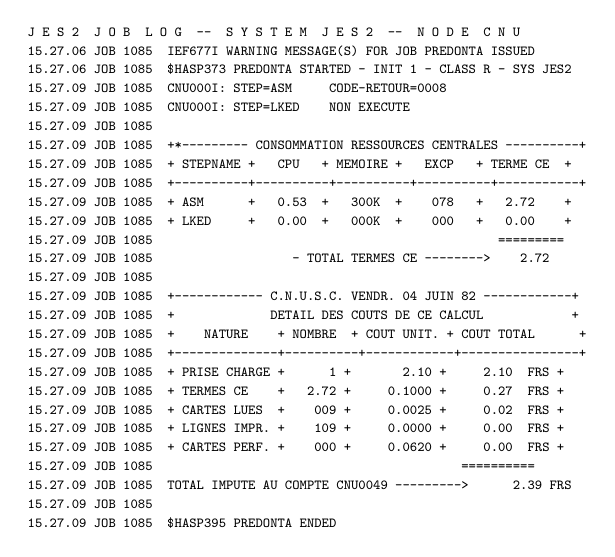
\begin{tikzpicture}[x=.08cm,y=.24cm]
\node[anchor=base west,inner sep=0pt,font=\tiny\ttfamily] at (0,0) {J\ E\ S\ 2\ \ J\ O\ B\ \ L\ O\ G\ \ --\ \ S\ Y\ S\ T\ E\ M\ \ J\ E\ S\ 2\ \ --\ \ N\ O\ D\ E\ \ C\ N\ U};
\node[anchor=base west,inner sep=0pt,font=\tiny\ttfamily] at (0,-1) {15.27.06\ JOB\ 1085\ \ IEF677I\ WARNING\ MESSAGE(S)\ FOR\ JOB\ PREDONTA\ ISSUED};
\node[anchor=base west,inner sep=0pt,font=\tiny\ttfamily] at (0,-2) {15.27.06\ JOB\ 1085\ \ \$HASP373\ PREDONTA\ STARTED\ -\ INIT\ 1\ -\ CLASS\ R\ -\ SYS\ JES2};
\node[anchor=base west,inner sep=0pt,font=\tiny\ttfamily] at (0,-3) {15.27.09\ JOB\ 1085\ \ CNU000I:\ STEP=ASM\ \ \ \ \ CODE-RETOUR=0008};
\node[anchor=base west,inner sep=0pt,font=\tiny\ttfamily] at (0,-4) {15.27.09\ JOB\ 1085\ \ CNU000I:\ STEP=LKED\ \ \ \ NON\ EXECUTE};
\node[anchor=base west,inner sep=0pt,font=\tiny\ttfamily] at (0,-5) {15.27.09\ JOB\ 1085\ \ };
\node[anchor=base west,inner sep=0pt,font=\tiny\ttfamily] at (0,-6) {15.27.09\ JOB\ 1085\ \ +*---------\ CONSOMMATION\ RESSOURCES\ CENTRALES\ ----------+};
\node[anchor=base west,inner sep=0pt,font=\tiny\ttfamily] at (0,-7) {15.27.09\ JOB\ 1085\ \ +\ STEPNAME\ +\ \ \ CPU\ \ \ +\ MEMOIRE\ +\ \ \ EXCP\ \ \ +\ TERME\ CE\ \ +};
\node[anchor=base west,inner sep=0pt,font=\tiny\ttfamily] at (0,-8) {15.27.09\ JOB\ 1085\ \ +----------+----------+----------+----------+-----------+};
\node[anchor=base west,inner sep=0pt,font=\tiny\ttfamily] at (0,-9) {15.27.09\ JOB\ 1085\ \ +\ ASM\ \ \ \ \ \ +\ \ \ 0.53\ \ +\ \ \ 300K\ \ +\ \ \ \ 078\ \ \ +\ \ \ 2.72\ \ \ \ +};
\node[anchor=base west,inner sep=0pt,font=\tiny\ttfamily] at (0,-10) {15.27.09\ JOB\ 1085\ \ +\ LKED\ \ \ \ \ +\ \ \ 0.00\ \ +\ \ \ 000K\ \ +\ \ \ \ 000\ \ \ +\ \ \ 0.00\ \ \ \ +};
\node[anchor=base west,inner sep=0pt,font=\tiny\ttfamily] at (0,-11) {15.27.09\ JOB\ 1085\ \ \ \ \ \ \ \ \ \ \ \ \ \ \ \ \ \ \ \ \ \ \ \ \ \ \ \ \ \ \ \ \ \ \ \ \ \ \ \ \ \ \ \ \ \ \ =========};
\node[anchor=base west,inner sep=0pt,font=\tiny\ttfamily] at (0,-12) {15.27.09\ JOB\ 1085\ \ \ \ \ \ \ \ \ \ \ \ \ \ \ \ \ \ \ -\ TOTAL\ TERMES\ CE\ -------->\ \ \ \ 2.72};
\node[anchor=base west,inner sep=0pt,font=\tiny\ttfamily] at (0,-13) {15.27.09\ JOB\ 1085\ \ };
\node[anchor=base west,inner sep=0pt,font=\tiny\ttfamily] at (0,-14) {15.27.09\ JOB\ 1085\ \ +------------\ C.N.U.S.C.\ VENDR.\ 04\ JUIN\ 82\ ------------+};
\node[anchor=base west,inner sep=0pt,font=\tiny\ttfamily] at (0,-15) {15.27.09\ JOB\ 1085\ \ +\ \ \ \ \ \ \ \ \ \ \ \ \ DETAIL\ DES\ COUTS\ DE\ CE\ CALCUL\ \ \ \ \ \ \ \ \ \ \ \ +};
\node[anchor=base west,inner sep=0pt,font=\tiny\ttfamily] at (0,-16) {15.27.09\ JOB\ 1085\ \ +\ \ \ \ NATURE\ \ \ \ +\ NOMBRE\ \ +\ COUT\ UNIT.\ +\ COUT\ TOTAL\ \ \ \ \ \ +};
\node[anchor=base west,inner sep=0pt,font=\tiny\ttfamily] at (0,-17) {15.27.09\ JOB\ 1085\ \ +--------------+----------+------------+----------------+};
\node[anchor=base west,inner sep=0pt,font=\tiny\ttfamily] at (0,-18) {15.27.09\ JOB\ 1085\ \ +\ PRISE\ CHARGE\ +\ \ \ \ \ \ 1\ +\ \ \ \ \ \ \ 2.10\ +\ \ \ \ \ 2.10\ \ FRS\ +};
\node[anchor=base west,inner sep=0pt,font=\tiny\ttfamily] at (0,-19) {15.27.09\ JOB\ 1085\ \ +\ TERMES\ CE\ \ \ \ +\ \ \ 2.72\ +\ \ \ \ \ 0.1000\ +\ \ \ \ \ 0.27\ \ FRS\ +};
\node[anchor=base west,inner sep=0pt,font=\tiny\ttfamily] at (0,-20) {15.27.09\ JOB\ 1085\ \ +\ CARTES\ LUES\ \ +\ \ \ \ 009\ +\ \ \ \ \ 0.0025\ +\ \ \ \ \ 0.02\ \ FRS\ +};
\node[anchor=base west,inner sep=0pt,font=\tiny\ttfamily] at (0,-21) {15.27.09\ JOB\ 1085\ \ +\ LIGNES\ IMPR.\ +\ \ \ \ 109\ +\ \ \ \ \ 0.0000\ +\ \ \ \ \ 0.00\ \ FRS\ +};
\node[anchor=base west,inner sep=0pt,font=\tiny\ttfamily] at (0,-22) {15.27.09\ JOB\ 1085\ \ +\ CARTES\ PERF.\ +\ \ \ \ 000\ +\ \ \ \ \ 0.0620\ +\ \ \ \ \ 0.00\ \ FRS\ +};
\node[anchor=base west,inner sep=0pt,font=\tiny\ttfamily] at (0,-23) {15.27.09\ JOB\ 1085\ \ \ \ \ \ \ \ \ \ \ \ \ \ \ \ \ \ \ \ \ \ \ \ \ \ \ \ \ \ \ \ \ \ \ \ \ \ \ \ \ \ ==========};
\node[anchor=base west,inner sep=0pt,font=\tiny\ttfamily] at (0,-24) {15.27.09\ JOB\ 1085\ \ TOTAL\ IMPUTE\ AU\ COMPTE\ CNU0049\ --------->\ \ \ \ \ \ 2.39\ FRS};
\node[anchor=base west,inner sep=0pt,font=\tiny\ttfamily] at (0,-25) {15.27.09\ JOB\ 1085\ \ };
\node[anchor=base west,inner sep=0pt,font=\tiny\ttfamily] at (0,-26) {15.27.09\ JOB\ 1085\ \ \$HASP395\ PREDONTA\ ENDED};

\end{tikzpicture}}
\diagram{\begin{tikzcd}\Delta\arrow[d,very thick]\\{}\end{tikzcd}}
\mspage{19}

\scanpage{21}
\mspage{\textcircled{b}}
we may assume $Y$ is a $(\underline W)$-Kan object of $\widehat A$, in which case $\operatorname{Hom}_{\mathrm{Hot}}(X,Y)\simeq\overline{\operatorname{Hom}}(X,Y)$ (homotopy classes of maps). Moreover, because of the assumption on $Y$, \inserted{the} homotopy relation \deleted{of}\inserted{among} maps $X\longrightarrow Y$ is \deleted{equivalent}\inserted{the same} \unsure{as} elementary homotopy.

Surjectivity of $(*)$? We get maps $g_0,g_1\cdots$
\diagram{\begin{tikzcd}
X_0\arrow[r,hook]\arrow[dr,"g_0"']&X_1\arrow[r,hook]\arrow[d,"g_1"]&X_2\arrow[r,hook]\arrow[dl,"g_2"]&{}\\
&Y&&
\end{tikzcd}}
\diagram{\begin{tikzcd}&X_n\arrow[r,no head,"f_n"]\arrow[dl,"g_n"']&X_{n+1}\arrow[dl,"g_{n+1}"]\\{}&{}&\end{tikzcd}}
such that $g_{n+1}f_n\sim g_n$ for any $n$, the question is to find \deleted{a representative} for each $n$ a $g'_n\sim g_n$ such that \uline{equality} $g'_{n+1}f_n=g'_n$ holds. This brings us to the slightly more general situation (where $i:X\longrightarrow X'$ is $f_n:X_n\longrightarrow X_{n+1}$, and $p:Y\longrightarrow Y'$ is the can. $Y\longrightarrow e$, and $g=g_n$, $\varphi=g_{n+1}$)
\diagram{\begin{tikzcd}
X\arrow[r,"g"]\arrow[d,"i"']&Y\arrow[d,"p"]\\
X'\arrow[r,"g'"']\arrow[ur,dashed,"\deleted{\unsure{g}}\varphi"]&Y'
\end{tikzcd}}
where $i$ is a cofibration, $p$ \unsure{is} a fibration, and the two triangles commutative up to homotopy
\[\varphi i\overset k\sim g\qquad p\varphi\overset h\sim g'\]
(we assume $X,X'$ cofibrant, $Y,Y'$ fibrant, so that $\overset l\sim$ and $\overset r\sim$ are the same, --- we look at the situation in any model category)

May we find a $\overline\varphi:X'\longrightarrow Y$ \inserted{homotopic to $\varphi$,} s.th. the two triangles commute:
\[\varphi i=g,\quad p\varphi=g'\qquad?\]
\margin{$\overline\varphi\sim\varphi$,}
\figure{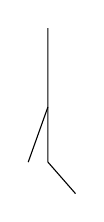
\begin{tikzpicture}\draw(0,1)--(0,-.7)--(.35,-1.1);\draw(0,0)--(-.25,-.7);\end{tikzpicture}}
Now this is about

\deleted{Let $\overline{X'}$ be a cylinder object over $X'$}

exactly the content of Quillen's version of ``covering homotopy extension theorem'' for simplicial closed model categories (prop. 4 of Ch. \uline{\unsure{II|I}}, pg \unsure{2.4|2.9}) --- although it was a little hard to make a sense of it, the way he states it

\margin{\deleted{\unsure{iff}} There is such a possibility, iff we can find $k$ and $h$ s.th. the two resulting homotopies $p\circ k$ and $h\circ(i\otimes\unsure{J|I})^{\unsure{o}}:\ p\varphi i\longrightarrow pg=g'i$ are homotopic! This is \unsure{possibly} not always satisfied!}
\figure{\begin{tikzpicture}[scale=.5]
\draw[->](0,0)--(0,4)--(1,4);\draw(.2,2.8)--(-.2,2.8) (.2,2.65)--(-.2,2.65) (.2,2.5)--(-.2,2.5) (.2,2.35)--(-.2,2.35);
\draw(1.3,0)..controls(1.1,.1)and(1.1,.3)..(1.3,.4)--(1.3,1.1)..controls(1.4,1.3)and(1.45,1.3)..(1.3,1.5)--(1.3,2.3);
\draw(3.6,0)..controls(3.8,.2)and(3.8,.4)..(3.6,.6)--(3.6,1.2)..controls(3.5,1.35)and(3.5,1.5)..(3.6,1.65)--(3.6,2.3);
\draw[->](1.5,2.5)..controls(2,2.8)and(2.4,2.8)..(2.8,2.5);
\end{tikzpicture}}
\mspage{20}

\scanpage{22}
\diagram{\begin{array}{rll}
\texttt{1}&\texttt{//PREDONTA JOB CNU0049-PREDONT,TIME=(0,3),CLASS=R}&\texttt{JOB 1085}\\
\texttt{2}&\texttt{// EXEC ASMFCL}&\texttt{00000020}\\
\texttt{3}&\texttt{XXASMFCL PROC MAC='SYS1.MACLIB',MAC1='CNU1.MACLIB'}&\texttt{00010071}\\
\texttt{}&\texttt{*** REFER SYS1.PROCLIB(ASMFCL)}&\texttt{00020000}\\
\texttt{}&\texttt{*** COMPID SYSTEM}&\texttt{00030000}\\
\texttt{}&\texttt{*** DOC THIS PROCEDURE EXECUTES THE ASSEMBLER AND THE LINKAGE}&\texttt{00040000}\\
\texttt{}&\texttt{*** EDITOR.}&\texttt{00050000}\\
\texttt{}&\texttt{***}&\texttt{00060000}\\
\texttt{4}&\texttt{XXASM EXEC PGM=IFOX00,PARM=OBJ}&\texttt{00070075}\\
\texttt{5}&\texttt{//ASM.SYSLIB DD DSN=CNU2.MODULEF.UTIMS,DISP=SHR}&\texttt{00000030}\\
\texttt{}&\texttt{X/SYSLIB DD DSN=\&MAC,DISP=SHR}&\texttt{00080070}\\
\texttt{6}&\texttt{// DD DSN=SYS1.MACLIB,DISP=SHR       -}&\texttt{00000040}\\
\texttt{}&\texttt{X/ DD DSN=\&MAC1,DISP=SHR}&\texttt{00090070}\\
\texttt{7}&\texttt{// DD DSN=CNU1.MACLIB,DISP=SHR}&\texttt{00000050}\\
\texttt{8}&\texttt{XXSYSUT1 DD DSN=\&\&SYSUT1,UNIT=VIO,SPACE=(CYL,(20,20))}&\texttt{00091076}\\
\texttt{9}&\texttt{XXSYSUT2 DD DSN=\&\&SYSUT2,UNIT=VIO,SPACE=(CYL,(10,10))}&\texttt{00092076}\\
\texttt{10}&\texttt{XXSYSUT3 DD DSN=\&\&SYSUT3,UNIT=VIO,SPACE=(CYL,(5,5))}&\texttt{00093076}\\
\texttt{11}&\texttt{XXSYSPRINT DD SYSOUT=*,DCB=BLKSIZE=1089}&\texttt{00130072}\\
\texttt{12}&\texttt{XXSYSPUNCH DD DUMMY}&\texttt{00140071}\\
\texttt{13}&\texttt{XXSYSGO DD DSN=\&\&OBJSET,UNIT=SYSDA,SPACE=(80,(200,50)),}&\texttt{00150070}\\
\texttt{}&\texttt{XX DISP=(MOD,PASS)}&\texttt{00160000}\\
\texttt{14}&\texttt{//ASM.SYSIN DD DSN=CNU2.MODULEF.UTIAS(IAND),DISP=SHR}&\texttt{00000060}\\
\texttt{15}&\texttt{XXLKED EXEC PGM=IEWL,PARM=(XREF,LET,LIST,NCAL),REGION=128K,}&\texttt{00170070}\\
\texttt{}&\texttt{XX COND=(8,LE,ASM)}&\texttt{00180071}\\
\texttt{16}&\texttt{XXSYSLIN DD DSN=\&\&OBJSET,DISP=(OLD,DELETE)}&\texttt{00190070}\\
\texttt{17}&\texttt{XX DD DDNAME=SYSIN}&\texttt{00200070}\\
\texttt{18}&\texttt{//LKED.SYSLMOD DD DSN=CNU2.MODULEF.UTIA(IAND),DISP=SHR}&\texttt{00000070}\\
\texttt{}&\texttt{X/SYSLMOD DD DSN=\&\&GOSET(GO),UNIT=3350,SPACE=(1024,(50,20,1)),}&\texttt{00210073}\\
\texttt{}&\texttt{XX DISP=(MOD,PASS)}&\texttt{00220000}\\
\texttt{19}&\texttt{XXSYSUT1 DD DSN=\&\&SYSUT1,UNIT=VIO,SPACE=(1024,(50,20))}&\texttt{00230070}\\
\texttt{20}&\texttt{XXSYSPRINT DD SYSOUT=*,DCB=(RECFM=FB,LRECL=121,BLKSIZE=1210)}&\texttt{00240072}\\
\texttt{}&\texttt{//}&\texttt{00000080}
\end{array}}

\diagram{\begin{tikzcd}
A \arrow[r,"\unsure{a}"] \arrow[d,very thick,"\mathrm{cof}"'] & X \arrow[d,very thick,"p"]\\
A\times I \arrow[r,"h"'] \arrow[ur,very thick] & Y
\end{tikzcd}}
\figure{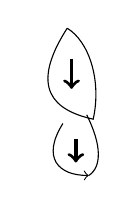
\begin{tikzpicture}[scale=.55]
\draw (0,2.8) .. controls (-.9,1.4) and (-.3,.9) .. (.6,.7) .. controls (.8,1.6) and (.5,2.5) .. (0,2.8);
\draw[->,very thick] (.1,2.1)--(.1,1.4);
\draw[->] (-.1,.6) .. controls (-.6,-.2) and (-.2,-.6) .. (.5,-.6);
\draw (.45,.8) .. controls (.8,.1) and (.8,-.4) .. (.5,-.6);
\draw[->,very thick] (.2,.25)--(.2,-.3);
\end{tikzpicture}}
\margin{$\unsure{\mathrm{fib}}$}
\diagram{\begin{tikzcd}
A & X \arrow[l]\\
A^I \arrow[u,"\deleted{\unsure{\partial_1}}\partial_0"'] & Y \arrow[l,very thick] \arrow[u,very thick,"\mathrm{cofib.}"]
\end{tikzcd}}
\figure{\begin{tikzpicture}
\draw (0,0)--(.3,.8)--(.4,.4);
\node at (2,0) {$\unsure{Y_x}$};
\end{tikzpicture}}
\diagram{\begin{tikzcd}
A \arrow[r,very thick] \arrow[d,very thick] & X \arrow[d,very thick]\\
B \arrow[r] \arrow[ur,very thick] & Y
\end{tikzcd}}
\mspage{21}

\scanpage{23}
\figure{
\begin{tikzpicture}\node[draw,circle] {$\mspage{\unsure{e|c}}$};\end{tikzpicture}}
\diagram{\begin{tikzcd}[column sep=large,row sep=huge]
X \arrow[r,bend left=24,"g_0=\varphi i"{name=t}]
  \arrow[r,bend right=24,"g_1=g"'{name=b}] \arrow[d,"i"'] & Y \arrow[d,"p"]\\
X' \arrow[ur,-,bend left=18,"\theta_0=\varphi"]
   \arrow[ur,dashed,"\theta_1=\bar\varphi"']
   \arrow[r,bend left=24,"g'_0=p\varphi"{name=u}]
   \arrow[r,bend right=24,"g'_1=g'"'{name=v}] & Y'
\arrow[from=t,to=b,"k"',shorten <=3pt,shorten >=3pt]
\arrow[from=b,to=t,shift right=8pt,shorten <=4pt,shorten >=4pt]
\arrow[from=u,to=v,"\unsure{h}"',shorten <=3pt,shorten >=3pt]
\arrow[from=v,to=u,shift left=8pt,shorten <=4pt,shorten >=4pt]
\end{tikzcd}}
We know \inserted{by assumption} there exist \inserted{simplicial} homotopies
\[
k:g_0=\varphi i\longrightarrow g_1=g\qquad\unsure{\text{and}}
\]
\[
h:g'_0=p\varphi\longrightarrow g'_1=g'.
\]
All we have to do, is to check that we can choose these homotopies \uline{compatible} with $i$ and $p$.
\margin{But in case $Y'$ is the final object, \deleted{\unsure{considering that}} \inserted{we are through!}}
\figure{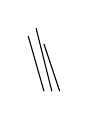
\begin{tikzpicture}\draw (0,0)--(-.2,.7);\draw (.1,0)--(-.1,.8);\draw (.2,0)--(0,.6);\end{tikzpicture}}
\deleted{\diagram{\begin{tikzcd}[column sep=small]
(X\amalg X) \arrow[d,"\mathrm{cofib?}"] & \amalg & (X'\amalg X') \arrow[d,"\mathrm{cofib?}"',"\unsure{=}"]\\
X\otimes J & \amalg \arrow[d] & X'\otimes J \arrow[r] & (Y\otimes J)\amalg\unsure{\bar\theta}\\
Y & \amalg & Y'
\end{tikzcd}}}
diagram
\diagram{\begin{tikzcd}
X\otimes J \arrow[r,"k"] \arrow[d,"i\otimes J"'] \arrow[dr,bend left=9] \arrow[dr,bend right=9] & Y \arrow[d,"p"]\\
X'\otimes J \arrow[r,"h"'] & Y'
\end{tikzcd}}
\deleted{which a priori is \uline{not} commutative but only commutative \deleted{\unsure{for}} on $X\amalg X\longrightarrow X\otimes J$}
\deleted{\diagram{\begin{tikzcd}
X\otimes J \arrow[r,"k"] \arrow[d,"i\otimes J"'] & Y \arrow[d,"p"]\\
X'\otimes J \arrow[r,"h"'] & Y'
\end{tikzcd}}}
\deleted{\diagram{\begin{tikzcd}[row sep=large]
X\amalg X \arrow[d] \arrow[dr,bend left=18,"u=(g_0,g_1)"] & \\
X\otimes J \arrow[r,dashed,-,"h'!"] \arrow[d,"i\otimes J"'] & Y \arrow[d,"p"]\\
X'\otimes J \arrow[r,"h"'] & Y'
\end{tikzcd}}}
\deleted{This diagram is commutative and we look for $h'$ which keeps it commutative.}
\deleted{We invert the problem, \deleted{\unsure{forgetting}} \inserted{\unsure{shortcircuiting}} $X'\otimes J$ by the arrow $h\circ(i\otimes J)=v$.}
\deleted{We know there is a \deleted{\unsure{and we want a}} $k$ s.th. $kj=u$, but \unsure{unfortunately} $ph\ne v$; only $pk\overset{s}{\sim}v$}
\deleted{(But in case $Y'$ is final object, we are already through!)}
\deleted{\diagram{\begin{tikzcd}
X\amalg X \arrow[r,"u=(g_0,g_1)"] \arrow[d,"j", "\text{\uuline{non} trivial cofibration}"'] & Y \arrow[d,"p\ \text{fibration}"]\\
X\otimes J \arrow[r,"v"'] \arrow[ur,dashed,"h'?"] & Y'
\end{tikzcd}}}
\margin{\deleted{\unsure{\times 0}}}
\figure{\begin{tikzpicture}[scale=.6]
\draw (0,12)--(2,13);\draw (0,10)--(4,13);\draw (0,7)--(1,8);
\draw (1,8)--(6,11);\draw (3,13)..controls(4,12.7)and(5,12.5)..(5.5,12);
\draw (0,6)--(8,-1);\draw (2,-1)--(10,8);
\end{tikzpicture}}
\mspage{22}

\scanpage{24}
\diagram{\begin{tikzcd}
X \arrow[r,bend left=15,"g_0=\varphi i"] \arrow[r,bend right=15,"g_1=\unsure{\varphi|\psi}i"'] \arrow[d] & Y \arrow[d]\\
X' \arrow[r,bend left=20,"g'_0=g'"] \arrow[r,bend right=20,"g_1=p\unsure{\varphi|\psi}"'] & Y'
\end{tikzcd}}
\diagram{\begin{tikzcd}[row sep=large]
X \arrow[r,bend left=25,"g_0=\varphi i"{name=t}] \arrow[r,bend right=25,"g_1=g"'{name=b}] \arrow[d,very thick,"i"'] & \deleted{X}Y \arrow[d,"p"]\\
X' \arrow[ur,-,bend left=20,"\varphi"] \arrow[r,bend left=25,"g'_0=p\varphi"{name=u}] \arrow[r,bend right=25,"g'_1=g'"'{name=v}] & Y'
\arrow[from=t,to=b,"k"',shorten <=2pt,shorten >=2pt]
\arrow[from=b,to=t,shift right=7pt,shorten <=3pt,shorten >=3pt]
\arrow[from=u,to=v,"h"',shorten <=2pt,shorten >=2pt]
\end{tikzcd}}
\diagram{\begin{array}{l}
\texttt{STMT NO. MESSAGE}\\
\texttt{-}\\
\texttt{5 IEF653I SUBSTITUTION JCL - DSN=SYS1.MACLIB,DISP=SHR}\\
\texttt{6 IEF653I SUBSTITUTION JCL - DSN=CNU1.MACLIB,DISP=SHR}\\
\texttt{20 IEF686I DDNAME REFERRED TO ON DDNAME KEYWORD IN PRIOR STEP WAS NOT RESOLVED}\\
\texttt{IEF236I ALLOC. FOR PREDONTA ASM}\\
\texttt{IEF237I 353 ALLOCATED TO SYSLIB}\\
\texttt{IEF237I 141 ALLOCATED TO}\\
\texttt{IEF237I 352 ALLOCATED TO}\\
\texttt{IEF237I VIO ALLOCATED TO SYSUT1}\\
\texttt{IEF237I VIO ALLOCATED TO SYSUT2}\\
\texttt{IEF237I VIO ALLOCATED TO SYSUT3}\\
\texttt{IEF237I JES2 ALLOCATED TO SYSPRINT}\\
\texttt{IEF237I DMY ALLOCATED TO SYSPUNCH}\\
\texttt{IEF237I 142 ALLOCATED TO SYSGO}\\
\texttt{IEF237I 351 ALLOCATED TO SYSIN}\\
\texttt{IEF142I PREDONTA ASM - STEP WAS EXECUTED - COND CODE 0008}\\
\texttt{IEF285I CNU2.MODULEF.UTIMS KEPT}\\
\texttt{IEF285I VOL SER NOS= SYSPPP.}\\
\texttt{IEF285I SYS1.MACLIB KEPT}\\
\texttt{IEF285I VOL SER NOS= SYSRES.}\\
\texttt{IEF285I CNU1.MACLIB KEPT}\\
\texttt{IEF285I VOL SER NOS= CNU001.}\\
\texttt{IEF285I SYS82155.T152706.RA000.PREDONTA.SYSUT1 DELETED}\\
\texttt{IEF285I SYS82155.T152706.RA000.PREDONTA.SYSUT2 DELETED}\\
\texttt{IEF285I SYS82155.T152706.RA000.PREDONTA.SYSUT3 DELETED}\\
\texttt{IEF285I JES2.JOB01085.\unsure{S00101|SO0101} SYSOUT}\\
\texttt{IEF285I SYS82155.T152706.RA000.PREDONTA.OBJSET PASSED}\\
\texttt{IEF285I VOL SER NOS= PUBL01.}\\
\texttt{IEF285I CNU2.MODULEF.UTIAS KEPT}\\
\texttt{IEF285I VOL SER NOS= CNU002.}\\
\texttt{IEF373I STEP /ASM / START 82155.1527}\\
\texttt{IEF374I STEP /ASM / STOP 82155.1527 CPU 0MIN 00.53SEC SRB 0MIN 00.01SEC VIRT 300K SYS 268K}\\
\texttt{CNU000I DETAIL EXCPS: 953----004 741----011 352----000 VIO----038 VIO----009 VIO----008 JES----??? JES----???}\\
\texttt{142----005 951----003}\\
\strut\\
\texttt{IEF202I PREDONTA LKED - STEP WAS NOT RUN BECAUSE OF CONDITION CODES}\\
\texttt{IEF272I PREDONTA LKED - STEP WAS NOT EXECUTED.}\\
\texttt{IEF373I STEP /LKED / START 82155.1527}\\
\texttt{IEF374I STEP /LKED / STOP 82155.1527 CPU 0MIN 00.00SEC SRB 0MIN 00.00SEC VIRT 0K SYS 0K}\\
\strut\\
\texttt{IEF237I 142 ALLOCATED TO SYS00001}\\
\texttt{IEF285I SYS82155.T152709.RA000.PREDONTA.R0000001 KEPT}\\
\texttt{IEF285I VOL SER NOS= PUBL01.}\\
\texttt{IEF285I SYS82155.T152706.RA000.PREDONTA.OBJSET DELETED}\\
\texttt{IEF285I VOL SER NOS= PUBL01.}\\
\texttt{IEF375I JOB /PREDONTA/ START 82155.1527}\\
\texttt{IEF376I JOB /PREDONTA/ STOP 82155.1527 CPU 0MIN 00.53SEC SRB 0MIN 00.01SEC}
\end{array}}
\mspage{23}

\scanpage{25}
\figure{\begin{tikzpicture}\node[draw,ellipse] {$\mspage{d}$};\end{tikzpicture}}
Returning to our initial pb, we get
\[
\deleted{\unsure{\lim}}\operatorname{Hom}(X_\infty,Y)\mathbin{-}\varprojlim\operatorname{Hom}(X_i,Y)
\]
\uline{surjective} (using strongly that the transition morphisms $X_i\mathbin{-}X_{i+1}$ are cofibrations). To prove it injective, let
\[
f,f':X_\infty\longrightarrow Y\qquad f_i=f|X_i,\quad f'_i=f'|X_i
\]
we have to prove that $f_i\sim f'_i\quad\forall i$, implies $f\sim f'$.

Consider
\diagram{\begin{tikzcd}[column sep=large]
\underbrace{X_\infty\times\Delta^{(1)}}_{B} & \underset{\mathrm{cofib.}}{\supset} & \underbrace{X_\infty\amalg X_\infty}_{A} \arrow[dl,-,sloped,"(f,f')"]\\
&Y&
\end{tikzcd}}
we want to extend to $X_\infty\times\Delta(1)$, and we know it is possible upon $X_i\times\Delta(1)\quad\forall i$.
\diagram{\begin{tikzcd}[column sep=small]
B & \supset & A\\
\vdots & & \vdots\\
B_{i+1} \arrow[d,"\mathrm{cofib}"'] & \supset & A_{i+1}\arrow[d,"\mathrm{cofib}"]\\
B_i & \underset{\mathrm{cofib.}}{\supset} & A_i
\end{tikzcd}}
We have to extend stepwise given homotopies. The problem is to construct $h_{i+1}$ extending $h'_{i+1}$
\figure{\begin{tikzpicture}\draw[->] (0,.6)--(.1,0);\end{tikzpicture}}
\diagram{\begin{tikzcd}[row sep=large,column sep=large]
A_i \arrow[r,hook,-] \arrow[d,hook] \arrow[dd,bend right=35,"\unsure{\varphi_i|\psi_i}"'] & B_i \arrow[d,hook] & \\
A_{i+1} \arrow[r,hook,-,""{name=s}] \arrow[d,"\varphi_{\unsure{i-1|i+1}}"'] & B'_{i+1}\arrow[r,hook,-] \arrow[dl,"h'_{i+1}"] & B_{\unsure{i-1|i+1}}\arrow[dll,dashed,bend left=15,"h_{\unsure{i-1|i+1}}?"]\\
Y' & &
\arrow[from=s,to=1-2]
\end{tikzcd}}
\[
\unsure{h'\!\!\!/}\qquad=B_i\amalg_{A_i}A_{\unsure{i-1|i+1}}
\]
\deleted{\diagram{\begin{tikzcd}& {}\arrow[dl,bend left=10,"\unsure{h?}"]\arrow[dl,bend right=10]\\{}&\end{tikzcd}}}
\figure{
\begin{tikzpicture}\draw (0,0)--(.9,.7)--(.15,.2)--(1,1)--(.1,.1)--(.7,.7);\end{tikzpicture}}
\diagram{\begin{array}{c}
\Delta(1)\times X_{i+1}\\
\cup\\
(\Delta(1)\times X_i)\cup(\{0\}\times X_{i+1})\cup(\{1\}\times X_{\unsure{i-1|i+1}})
\end{array}}
\diagram{\begin{tikzcd}
Y\arrow[r,hook,-,shift right=.6pt]\arrow[r,<-,shift left=.6pt]&Z_0\arrow[r,hook,-]&Z_1\arrow[r,hook,-]&Z_2\mathbin{\cdots-}
\end{tikzcd}}
Assume $\forall i$, $\exists$ retraction $Z_i\mathbin{-}Y$

Is there a retraction $Z_\infty\longrightarrow Y$?

\uline{not clear at all}, \unsure{on|our} \deleted{\unsure{contrary}} the whole point is to see that
\[
\varprojlim_i\pi_0\underline{\operatorname{Retr}}(\unsure{Z_i|Z},Y)\ne\varnothing.\mathbin{-}
\]
Ask Ronnie Brown!
\mspage{24}

\scanpage{26}
\hfill\texttt{PAGE 2}
\texttt{LOC OBJECT CODE ADDR1 ADDR2 STMT SOURCE STATEMENT}\hfill\texttt{ASM 0201 15.27 06/04/82}
\diagram{\begin{array}{llllllll}
\texttt{000000}&\texttt{}&\texttt{}&\texttt{}&\texttt{1}&\texttt{IAND START}&\texttt{}&\texttt{IAND...1}\\
\texttt{}&\texttt{}&\texttt{}&\texttt{}&\texttt{2}&\texttt{\$SAVE OPTION=FUN}&\texttt{}&\texttt{IAND...2}\\
\texttt{000000}&\texttt{}&\texttt{}&\texttt{}&\texttt{3+}&\texttt{CNOP 0,4}&\texttt{}&\texttt{\$SAVE.91}\\
\texttt{}&\texttt{}&\texttt{}&\texttt{00000}&\texttt{4+}&\texttt{USING *,15}&\texttt{}&\texttt{\$SAVE.92}\\
\texttt{000000}&\texttt{47F0 F00C}&\texttt{0000C}&\texttt{}&\texttt{5+}&\texttt{BC 15,*+12}&\texttt{}&\texttt{\$SAVE.94}\\
\texttt{000004}&\texttt{04}&\texttt{}&\texttt{}&\texttt{6+}&\texttt{DC AL1(4)}&\texttt{}&\texttt{\$SAVE.95}\\
\texttt{000005}&\texttt{C9C1D5C4404040}&\texttt{}&\texttt{}&\texttt{7+}&\texttt{DC CL7'IAND'}&\texttt{}&\texttt{\$SAVE.96}\\
\texttt{00000C}&\texttt{90EC D00C}&\texttt{0000C}&\texttt{}&\texttt{8+}&\texttt{STM 14,12,12(13)}&\texttt{}&\texttt{\$SAVE.97}\\
\texttt{000010}&\texttt{182D}&\texttt{}&\texttt{}&\texttt{9+}&\texttt{LR 2,13}&\texttt{}&\texttt{\$SAVE.99}\\
\texttt{000012}&\texttt{98DE F020}&\texttt{00020}&\texttt{}&\texttt{10+}&\texttt{LM 13,14,*+14}&\texttt{}&\texttt{\$SAV.100}\\
\texttt{000016}&\texttt{5020 D004}&\texttt{00004}&\texttt{}&\texttt{11+}&\texttt{ST 2,4(0,13)}&\texttt{}&\texttt{\$SAV.101}\\
\texttt{00001A}&\texttt{50D0 2008}&\texttt{00008}&\texttt{}&\texttt{12+}&\texttt{ST 13,8(0,2)}&\texttt{}&\texttt{\$SAV.102}\\
\texttt{00001E}&\texttt{07FE}&\texttt{}&\texttt{}&\texttt{13+}&\texttt{BCR 15,14}&\texttt{}&\texttt{\$SAV.103}\\
\texttt{000020}&\texttt{00000028}&\texttt{}&\texttt{}&\texttt{14+}&\texttt{DC A(SAV0001A)}&\texttt{}&\texttt{\$SAV.104}\\
\texttt{000024}&\texttt{00000070}&\texttt{}&\texttt{}&\texttt{15+}&\texttt{DC A(*+76)}&\texttt{}&\texttt{\$SAV.106}\\
\texttt{}&\texttt{}&\texttt{}&\texttt{}&\texttt{16+}&\texttt{DROP 15}&\texttt{}&\texttt{\$SAV.107}\\
\texttt{}&\texttt{}&\texttt{}&\texttt{00028}&\texttt{17+}&\texttt{USING *,13}&\texttt{}&\texttt{\$SAV.109}\\
\texttt{000028}&\texttt{00000000}&\texttt{}&\texttt{}&\texttt{18+}&\texttt{SAV0001A DC A(SAV0001B)}&\texttt{}&\texttt{\$SAV.110}\\
\texttt{}&\texttt{*** ERROR ***}&\texttt{}&\texttt{}&\texttt{}&\texttt{}&\texttt{}&\texttt{}\\
\texttt{00002C}&\texttt{}&\texttt{}&\texttt{}&\texttt{19+}&\texttt{DS 17F}&\texttt{}&\texttt{\$SAV.111}\\
\texttt{000070}&\texttt{5821 0000}&\texttt{00000}&\texttt{}&\texttt{20}&\texttt{L 2,0(1)}&\texttt{}&\texttt{IAND...3}\\
\texttt{000074}&\texttt{\unsure{5302|5802} 0000}&\texttt{00000}&\texttt{}&\texttt{21}&\texttt{L 0,0(2)}&\texttt{}&\texttt{IAND...4}\\
\texttt{000078}&\texttt{5821 0004}&\texttt{00004}&\texttt{}&\texttt{22}&\texttt{L 2,4(1)}&\texttt{}&\texttt{IAND...5}\\
\texttt{00007C}&\texttt{5402 0000}&\texttt{00000}&\texttt{}&\texttt{23}&\texttt{N 0,0(2)}&\texttt{}&\texttt{IAND...6}\\
\texttt{}&\texttt{}&\texttt{}&\texttt{}&\texttt{24}&\texttt{RETURN}&\texttt{}&\texttt{IAND...7}\\
\texttt{000080}&\texttt{07FE}&\texttt{}&\texttt{}&\texttt{25+}&\texttt{BR 14}&\texttt{RETURN}&\texttt{02000000}\\
\texttt{}&\texttt{}&\texttt{}&\texttt{}&\texttt{26}&\texttt{END}&\texttt{}&\texttt{IAND...8}
\end{array}}

\figure{
\begin{tikzpicture}[x=1cm,y=1cm]
\draw[red!60!black] (0,0)..controls(.4,-.17)and(.8,.16)..(1.5,.04)--(1.5,.22)..controls(1,-.07)and(.4,.02)..(.2,.02);
\draw[red!60!black] (.1,-.06)..controls(.5,-.2)and(1,.03)..(1.5,-.04);
\end{tikzpicture}}
\mspage{25}
